\documentclass[11pt,oneside,a4paper,openright]{book}

\usepackage[utf8]{inputenc}
\usepackage[T1]{fontenc}
\usepackage[english]{babel}


\usepackage{titlesec}
\usepackage{etoc}
\usepackage{amsmath}
\usepackage{url}
\usepackage{graphicx}
\usepackage[export]{adjustbox}
\usepackage{caption}
\usepackage{subcaption}
\usepackage{xcolor}
\usepackage{hyperref}
\hypersetup{
    colorlinks=true,
    linkcolor=cyan,
    urlcolor=blue,
    citecolor=cyan
}

\usepackage[margin=2.9cm,inner=3.4cm]{geometry}

%%\chapternumberfont{\tiny}
\chaptertitlefont{\Large}
%%\pagenumbering{roman}
\pagenumbering{arabic}

\begin{document}

\newcommand{\HRule}{\rule{\linewidth}{0.5mm}}

\begin{titlepage}

\begin{center}

% Upper part of the page

\includegraphics{frontmatter/unilogo}
%\unilulogo[1]
%\hfill
%\micslogo[1]

\vspace{1cm}

%\textsc{\LARGE University of Luxembourg}\\[1.0cm]
\textsc{\Large Faculty of Science, Technology and Medicine }\\[1.0cm]

\vspace{1cm}

% Title
\HRule \\[0.4cm]
{\huge \bfseries What Can a Swiped Word Tell Us More?}\\{\huge Predicting Demographical and Behavioral Traits from Shape-Writing Text Entry}
\HRule \\[1.5cm]


\begin{minipage}{0.8\textwidth}
\begin{center}
{\Large Thesis Submitted in Partial Fulfillment of the Requirements
for the Degree of Master in Information and Computer Sciences}
\end{center}
\end{minipage}

% use Prof. and Ass. Prof. as abbreviations for Professor and Associate Professor
% check csc.uni.lu/members for title
\vspace{4cm}
\begin{minipage}[t]{0.4\textwidth}
\begin{flushleft} \large
% the student who wrote the thesis
\emph{Author:}\\
Désirée Claire Annie \textsc{Lemarquis}
\end{flushleft}
\end{minipage}
\begin{minipage}[t]{0.4\textwidth}
\begin{flushright} \large
% supervisor and reviewer are defined in the mics regulations (see moodle)
\emph{Supervisor:} \\
Asst.~Prof.~Luis \textsc{Leiva} \\
\vspace{.5em}
\emph{Reviewer:} \\
Assoc.~Prof.~Christoph \textsc{Schommer} \\
\vspace{.5em}
% advisor is a person that helps in the daily supervision
\emph{Advisor:} \\
Dr.~Bereket Abera \textsc{Yilma}
\end{flushright}
\end{minipage}

\vfill

% Bottom of the page
% month of submission
{\large August 2022}

\end{center}

\end{titlepage}
\newpage\null\thispagestyle{empty}\newpage

\chapter*{Declaration of Authorship}

I hereby declare in lieu of an oath that the thesis submitted in partial fulfillment of the requirements for the Master in Information and Computer Sciences and entitled\newline

{\bfseries What Can a Swiped Word Tell Us More?}\\{Predicting Demographical and Behavioral Traits from Shape-Writing Text Entry}\newline

is original and the result of my own investigations. I have cited in proper and due form all used sources (e.g., ideas, equations, figures, text, tables, programs, algorithms). This work has not been submitted in whole or in part for another degree.\newline\newline

\begin{flushright}Luxembourg, August 2022\end{flushright}\\
\begin{flushright}Lemarquis Désirée Claire Annie\end{flushright}


\large
\chapter*{Acknowledgements}
\addcontentsline{toc}{chapter}{Acknowledgements}
Firstly, I would like to express my sincere gratitude to my supervisor Asst. Prof. Luis Leiva for offering this internship and choosing me as a candidate to work on it. I also could not have undertaken this journey without my advisor Dr. Bereket Abera Yilma. They both provided generously their knowledge and expertise, their patience as well as their time to have meetings. I would like to extend my sincere gratitude to thank Assoc. Prof. Christoph Schommer for reviewing my thesis.\\

The experiments presented in this work were carried out
using the HPC facilities of the University of Luxembourg: \url{http://hpc.uni.lu}\\

Lastly, I would like to express my gratitude to my family and friends for their love and support. I would also like to thank my dogs Marley and Simba for all their entertainment and emotional support.
\newpage


\chapter*{Abstract}
\addcontentsline{toc}{chapter}{Abstract}
%% Short summary of this work (max 250 words).
%% EXAMPLE: http://www.cbs.umn.edu/sites/default/files/public/downloads/Annotated_Nature_abstract.pdf

%% (1) One sentence providing a basic introduction to the field, comprehensible to a scientist in any discipline.
%% (2) One sentences of more detailed background, comprehensible to scientists in related disciplines.
%% (3) One sentence clearly stating the general problem being addressed by this particular study.
%% (4) One sentence summarising the main result (with the words “here we show” or their equivalent).
%% (5) One sentences explaining what the main result reveals in direct comparison to what was thought to be the case previously, or how the main result adds to previous knowledge.
%% (6) One sentences to put the results into a more general context.
%% (7) One sentences to provide a broader perspective, readily comprehensible to a scientist in any discipline.

Shape-writing (aka gesture typing or swiping) is a word-based text entry method for touchscreen keyboards.
It works by landing the finger on (or close to) the first character of the desired word
and then sliding over all the other character keys without lifting the finger until the last word character is reached.
This generates a trajectory of swiped characters on the keyboard layout
which can be translated to a meaningful word by a statistical decoder.
%
We hypothesize that swiping carries rich information about the user,
such as demographical (e.g. age or gender) and behavioral (e.g. swiping familiarity or input finger) information.
Nevertheless, this has not been explored yet, mainly because until very recently there were no public datasets.
Thus, we set out to explore what user information can be learned from a swiped word
using the only publicly available swiping dataset to date.
For this, we trained several sequence classifiers using different recurrent neural network architectures
to predict demographic and behavioral traits of users from swipe trajectories.
%
We show that our sequence classifiers are always performing better than a random classifier,
therefore a new research avenue opens for advanced user profiling on swiping data.
%
Currently swiping is supported by all mobile vendors and has millions of users,
so users may be inadvertently tracked at an unprecedented granularity.
%
We conclude that the cognitive and motor control mechanisms are embodied and reflected in swipe trajectories,
and that user privacy may be at risk by unethical mobile vendors or fishy soft keyboards.

%% Leave a newline after the the last sentence in the abstract before the keywords list.
\vspace{1em}
\textbf{Keywords:} Shape-writing; Gesture Typing; Text Entry; Biometrics; Neural Networks

\addcontentsline{toc}{chapter}{Contents}
\tableofcontents\newpage

\addcontentsline{toc}{chapter}{List of Figures}
\listoffigures\newpage

\addcontentsline{toc}{chapter}{List of Tables}
\listoftables\newpage


%%\pagenumbering{arabic}

%% ============================================================================
\chapter{Introduction}
\addcontentsline{lof}{chapter}{Introduction}
%% ============================================================================

%% Motivation: Why this work is important?
%% Brief summary of previous works (only the 2-3 key related works) -> why they are not enough?
%% Contributions: What do we propose in this paper?

\section{Background and Motivation}
Nowadays, mobile phones and screen based smart devices are a part daily life and indispensable tools for their users offering various features, functionalities, and usage possibilities. People use screen based smart devices such as phones and tablets for many different reasons e.g. to play games, to watch films or videos, to stay connected on social medias, to take pictures, and most importantly to communicate through calls, text messaging and emails.\\ %We notice that people tend to lose the focus on their environment  when they are typing messages on their phones.\\

In the human-computer interaction(HCI), the mobile text input represents the most intense and common task for which the speed needs to be taken in consideration. The speed of typing on a keyboard depends mostly on the user experience and the size of the device screen. The academic researchers as well as the information technology industry are always seeking to discover new efficient text entry methods. A new text entry method should require a minimal cognitive effort from new users to achieve a large-scale acceptance. It should also support skill development, i.e. the users performance improves through practice. Mobile vendors are trying to provide effective text entry services to their users. In recent years, all mobile vendors introduced a new concept called shape-writing to offer the possibility to their users to communicate faster by swiping rather than typing on the keyboard. \\


In the work of Palin et al.~\cite{Palin19}, they collected mobile text entry data from 37,370 participants that perfomed a web-based transcription task by typing 15 sentences each from the Enron phrase set. They showed in their study that text was entered at an average 36.17 words per minute(WPM). They presented us meaningful insights into the correlation of typing performance and various factors such as the use of Intelligent Text Entry(ITE) methods, e.g. swiping, by analyzing their large-scale dataset. In their analysis, they found out that more than half of the participants used a combination of ITEs, e.g. autocorrection, prediction or gesture. They showed that autocorrection and prediction were more preferred by the users, since their combination was used by 31.5\% of the participants. The best performance was 43.3 WPM by using only the autocorrection method. They discovered that only 1.9\% of the participants used swiping i.e. only 22\% of the total words were swiped.  The text was entered by shape-writing at an average of 32.2 WPM, but since the sample size for swiping is extremely small we do not consider this finding. The participants had the freedom to choose how they type i.e. by typing on keyboard, by using a single ITE(autocorrection, prediction, swiping) or a combination of different ITE.\\

On the other hand, Leiva et al.~\cite{Leiva21_swipe} conducted a study where the participants only performed shape-writing on 15 sentences each from the same phrase set. The participants swiped at an average of 39.82 WPM, and the fastest performance was reached with 72.89 WPM. This study proved to us that the mobile vendors introduced a fast typing concept, i.e. swiping, into their devices by comparing the average WPM from the swiping performance with previous typing performance. Thus, we were motivated to learn new things about the dataset of Leiva et al.~\cite{Leiva21_swipe}. We realized that we would be able to conduct an interesting study in Deep Learning about this new text entry method, e.g. shape-writing, since they not only made available swiping trajectories, but also the related user demographics. The concept of shape-writing is in simple words a practical text entry method, where a user writes texts on a graphical keyboard by performing gestures. In the next section, shape-writing will be explained in more details.  \newpage



\section{Shape Writing}

Shape-writing, also known as gesture typing, swype input, swipe to text, or just \emph{swiping} (for short),
is a prevalent mobile text entry method currently supported by all mobile vendors.
Contrary to regular touch typing,
where the user touches one key at a time and lifts up the finger to enter one character,
swiping is a \emph{word}-based text entry method:
The finger lands on (or close to) the first key of the desired word
and then, without lifting the finger from the keyboard,
it traverses (the vicinity of) all the keys until reaching the last character of the word,
generating a trajectory of touch points as a result.
See \autoref{fig:swipe-examples} for some examples.\\

\begin{figure*}[!ht]
    \centering
    \def\w{0.3\linewidth}

    \subfloat[\texttt{advice}]{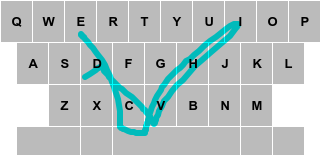
\includegraphics[width=\w]{imgs/vvr5s7lo8lhibvfm37q7vag4mb-advice-0.png}}\hfill
    \subfloat[\texttt{manchester}]{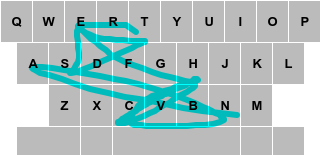
\includegraphics[width=\w]{imgs/vvr5s7lo8lhibvfm37q7vag4mb-manchester-0.png}}\hfill
    \subfloat[\texttt{tomorrow}]{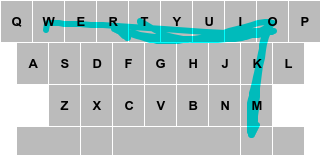
\includegraphics[width=\w]{imgs/vvr5s7lo8lhibvfm37q7vag4mb-tomorrow-0.png}}\hfill\\ \vspace{1cm}
    \subfloat[\texttt{wellcare}]{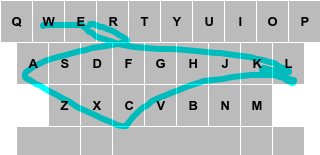
\includegraphics[width=\w]{imgs/vvr5s7lo8lhibvfm37q7vag4mb-wellcare-0.png}}\hspace{1cm}
    \subfloat[\texttt{download}]{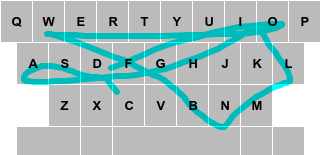
\includegraphics[width=\w]{imgs/vvr5s7lo8lhibvfm37q7vag4mb-download-0.png}}

    \caption{Examples of swiped word trajectories.}
    \label{fig:swipe-examples}
\end{figure*}

However, shape-writing is not extensively researched. Swiping performance has been researched in small-scale experiments~\cite{Reyal2015},in large-scale studies as one of many text methods~\cite{Palin19}, or using proprietary, undisclosed datasets~\cite{Quinn18}. In Reyal et al.~\cite{Reyal2015}, two popular mainstream mobile text entry methods, e.g. the Smart Touch Keyboard (STK) and the Smart Gesture Keyboard (SGK), were studied to gain information on their performance and user experience. Firstly, they analyzed their results of their lab-based text entry experiment that consisted of 10 sessions with 12 participants. Afterwards, they did an additional study with 12 different participants and with a new text input evaluation methodology that was based on the experience sampling method(ESM). The users installed for this study an Android app on their mobile phones. This app collected on a regular basis their text input performance and user experience from their daily activities for 4 weeks. They showed in their studies that text was entered at an average of 28 to 39 words per minute(WPM) with 1.0\% to 3.6\% uncorrected errors depending on the method and the user’s experience. They concluded that their studies were informative to discover different aspects of keyboard experience, and that it is more reliable to thoroughly evaluate the input technologies of current and future generations. In Palin et al.~\cite{Palin19}, we mentioned in the section before that that they collected mobile text entry data in a large-scale study. They analyzed the correlation of typing performance and various factors such as the use of ITE methods. We could not consider using their dataset since only 22\% of the overall data were performed by shape-writing. In Quinn et al.~\cite{Quinn18}, they developed a model that produces swiping input based on a human motor control theory of optimal control i.e. the human-drawn trajectories are modeled by minimizing the acceleration changes of the human hand movement from one point to another. Their model predicts the shapes and movements  for an arbitrary swiping task. Their minimum jerk theory of motor control is supported by their analysis of user-generated swiping trajectories from a proprietary, undisclosed dataset, which provided a qualitative and quantitative correlation between the user-drawn shapes and their theory. Thus, it is challenging to collect swiping trajectories since most mobile keyboards are vendor-locked and do not offer an API to collect swiping data.\\

Until now, there was no public swiping dataset where researchers could access raw movements dynamics such as the gesture path drawn on top of the keyboard or the time lapsed between consecutive swiped keys. Recently, Leiva et al.~\cite{Leiva21_swipe} released the largest dataset (1,300 participants) for conducting research on mobile swiping together with first observations of correlates of typing performance. Large-scale analyses of mobile interaction are relatively rare and mostly undertaken by commercial organizations that hold the datasets proprietary. There are notable exceptions ~\cite{Buschek18, Henze12, Dhakal18, Palin19} but they did not investigate swiping behavior. In Buschek et al.~\cite{Buschek18} they developed an Android keyboard app where they collected only typing information without the actual text. They analyzed typing biometrics, i.e. speed, auto correction, word predictions, etc., from their keyboard typing logs. In Henze et al.~\cite{Henze12} the users' typing behavior on the Android keyboard was studied by using the logs of their developed typing game. They also evaluated in the game's update how shifting touch events, modifying keys' labels, and visualizing the touched position affected the typing behaviour. In Dhakal et al.~\cite{Dhakal18} they investigated the users' typing behavior from the results of an online study. They found out that rollover typing is very common and that letter repetitions are slower to type than letter pairs with different hands or fingers~\cite{Dhakal18}. In Palin et al.~\cite{Palin19} they investigated as mentioned above for example the correlation of typing performance and various factors such as the use of swiping.\newpage

\section{Problem Statement}
Nowadays, shape-writing is supported by all mobile vendors. However, swiping datasets are challenging to find since gesture typing performance is not extensively researched. Additionally, most mobile keyboards are vendor-locked such that it is hard to collect a huge amount of swiping trajectories. We believe that swiping trajectories carry more information than just the shape-writing, i.e. they have the power to reveal explanatory information about the users’ demographics, and that users risk therefore their privacy by sharing their shape-writing data.\\

Thus, we hypothesize that swiping carries rich information about the user, such as demographical (e.g. age or gender) and behavioral (e.g. swiping familiarity or input finger) information. In this work we analyse the dynamics of swiping trajectories to model and predict different biometric traits, such as age, gender, nationality, English level, swiping familiarity, swiping hand, swiping finger or dominant hand. We investigate also how the systematical changes in popular architectural model choices influence the models ability to learn patterns about the different targets from our swiping data.




%% ============================================================================
\chapter{Related Work}
%% ============================================================================
%% What has been done before? Why is it not good enough?
%% We need to discuss at least 10 related papers.

Invented by Zhai and Kristensson in 2003~\cite{Zhai03},
swiping has become a widely adopted text entry method on mobile devices.
It well suits touch-based interaction, and relaxes the requirement of precisely acquiring a small key on a soft keyboard.
To date, this text entry method is supported by major commercial soft keyboards
including Google's Gboard, Microsoft' SwiftKey, and iOS's built-in keyboard on iPhones.\\

The research community has carried out a large amount of research on swiping techniques.
For example, swiping has been extended to support mid-air text entry~\cite{Markussen:2014:VMW}, eyes-free input~\cite{zhu2019sfree}, ring-based input~\cite{gupta2019rotoswype}, phone-tilting based input~\cite{yeo2017investigating}.
In addition to text entry, swiping has also been extended to support command input~\cite{kristensson2007command, alvina2017commandboard, cui2019hotstrokes},
by gesturing a shortcut related to the command name.
Such a method shows advantages in learnability compared with hotkey-based command input~\cite{cui2019hotstrokes}.\\

%% https://luis.leiva.name/web/docs/papers/handwriting-biometrics-icpr2020-preprint.pdf
Leiva et al.~\cite{Leiva20_biometrics} showed that accurate detection of human movements
has more to do with \emph{how} users write, rather than \emph{what} they write.
They concluded that it is better to use recurrent models than convolutional models for biometric classification,
as recurrent models capture the inherent movement dynamics.
However, they only explored one shallow architecture,
based on Bidirectional Gated Recurrent Unit (BiGRU) cells,
in the context of binary classification of human vs. fake handwriting.
Therefore, it is unclear what design choices over the different hyperparameters
(e.g. number of hidden layers, type of recurrent cell, number of hidden units, learning rates, etc.)
may affect classification performance.
In this work we perform an exhaustive investigation in this regard.

\section{Biometrics Prediction}

%% Leiva et al.~\cite{Leiva21_swipe} mentions previous work about text entry:
%% https://luis.leiva.name/web/docs/papers/shapewriting-mobilehci2021-preprint.pdf

There is a large body of work that demonstrates that our digital footprints,
including e.g. the websites we visit or the text we enter in social media,
may help derive personally identifiable information like gender, age, location, or even political orientation.
Existing literature related to online privacy provides insights around topics such as
information leakage while surfing the web using desktop computers~\cite{Starov_2016}
or mobile devices~\cite{Leung_2016}.\\

%% Leiva et al.~\cite{Leiva21_privacy} provide an extensive literature review of biometric-like classifiers:
%% https://luis.leiva.name/web/docs/papers/mouseprivacy-chiir2021-preprint.pdf
Leiva et al.~\cite{Leiva21_privacy} showed that our mouse movements may reveal who we are.
They developed a computational model based on BiGRU cells and were able to classify the age and
gender of the users
with 65.3\% and 64.1\% of accuracy, respectively.
%These results suggest that our digital privacy is at risk,
%since today it has become trivial to acquire mouse movements unobtrusively and at large scale.
%Furthermore, developing sophisticated classifiers is easier than ever thanks to libraries like Scikit-learn, Tensorflow, or Pytorch.
Recent work by White et al.~\cite{White18} and Gajos et al.~\cite{Gajos20}
could detect neurodegenerative disorders from mouse cursor movements,
showing how our ``digital phenotypes'' could be used as adjunctive screening tools.\\

Chen et al.~\cite{Chen_2001} were the first to notice a strong relationship between gaze position and cursor position during web browsing.
Mueller and Lockerd~\cite{Mueller01_cheese} investigated the use of mouse tracking to visualize and (manually) infer the users' interests.
Since then, researchers have noted the utility of mouse cursor analysis
as a low-cost and scalable proxy of eye gaze~\cite{Huang12_search, Huang12_align, Navalpakkam13_layout}.
Several works have investigated closely the utility of mouse cursor data in web search~\cite{Arapakis16_dds, Chen17_satisfaction, Liu15_opinions}
and web page usability evaluation~\cite{Arroyo06_usab, Atterer06_move, Leiva11_adapt},
two of the most prominent use cases of this technology.
Mouse biometrics is another active research area that has recently shown how to identify an individual
by analyzing their mouse movements in controlled settings~\cite{Kratky18_biom, Lu17_biom}.
This is the research line we focus on in this work.\\

Objective measurements of attentional processes are increasingly being used to explain or predict user behavior.
Early mouse cursor tracking systems began by logging click events only (coordinates and timestamp)
and using these events to assess what information users were interested in.
However, it was soon realized that click data provide an incomplete picture of user interaction.
A mouse click is often preceded by several interactions such as scrolling, hovers, movements, etc.
and thus can lead to a better overall understanding of the user's thought process.\\

In what follows, we review research efforts that have focused on mouse cursor analysis
to infer user interest, visual attention, emotions, and demographic variables like gender or age, on a desktop setting.
We hypothesize that swiped word trajectories carry the same rich information about the user.

\section{Inferring User Interest}
\label{sec:interest}

For a long time, commercial search engines have been interested in how users interact with Search Engine Result Pages (SERPs),
to anticipate better placement and allocation of ads in sponsored search or to optimize the content layout.
Early work considered simple, coarse-grained features derived from mouse cursor data
to be surrogate measurements of user interest~\cite{Claypool01_iii, Shapira06_ii}.
Follow-up research transitioned to more fine-grained mouse cursor features~\cite{Guo08_query,
Guo10_buy}
that were shown to be more effective.
These approaches have been directed at predicting open-ended tasks
like search success~\cite{Guo12_success} or search satisfaction~\cite{Liu15_opinions}.
In a similar vein, Huang et al.~\cite{Huang12_search, Huang11_clicks}
modeled mouse cursor interactions and extended click models to compute more accurate relevance judgements of search results.
Mouse cursor position is mostly aligned to eye gaze,
especially on SERPs~\cite{Guo12_rel, Speicher13_rel},
and that can be used as a good proxy for predicting good and bad abandonment~\cite{Diriye12_leaving}.

\section{Inferring Visual Attention}
\label{sec:attention}

Mouse cursor tracking has been also used to survey the visual focus of users in sponsored search,
thus revealing valuable -- and at the same time sensitive -- information
regarding the distribution of user attention over the various SERP components.
Despite the technical challenges that arise from this analysis,
previous work has shown the utility of mouse movement patterns
to measure within-content engagement~\cite{Arapakis14_news}
and predict reading experiences~\cite{Arapakis14_gestures, Hauger11}.
Lagun et al.~\cite{Lagun14_motifs} introduced the concept of motifs,
or frequent cursor subsequences, in the estimation of search result relevance.
Similarly, Liu et al.~\cite{Liu15_opinions} applied the motifs concept to SERPs
and predicted search result utility, searcher effort, and satisfaction at a search task level.
Boi et al.~\cite{Boi2016} proposed a method for predicting whether the user is looking at the content pointed by the cursor,
exploiting the mouse cursor data and a segmentation of the contents in a web page.
Lastly, Arapakis et al.~\cite{Arapakis16_dds, Arapakis20_ppa}
investigated user engagement with direct displays on SERPs
and provided further evidence that supports the utility of mouse cursor data
for measuring user attention at a display-level granularity.

\section{Inferring Emotional State}
\label{sec:emotion}

Although the connection between mouse cursor movements and the underlying psychological states has been a topic of research
since the early 90s~\cite{Accot97_fitts, Card87_mouse},
some studies have investigated the utility of mouse cursor data for predicting the user's emotional state.
For example, Zimmermann et al.~\cite{Zimmermann2003} investigated the effect of induced affective states
on the motor-behavior of online shoppers and found that the total duration of mouse cursor movements
and the number of velocity changes were associated to the experienced arousal.
Kaklauskas et al.~\cite{Kaklauskas2009}
created a system that extracts physiological and motor-control parameters
from mouse cursor interactions and then triangulated those with psychological data taken from self-reports,
to analyse correlations with users' emotional state and labour productivity.
In a similar line, Azcarraga et al.~\cite{Azcarraga12_brain} combined electroencephalography signals and mouse cursor interactions
to predict self-reported emotions like frustration, interest, confidence and excitement.
Yamauchi et al.~\cite{Yamauchi13_anxiety} studied the relationship between mouse cursor trajectories and generalized anxiety in human subjects.
Lastly, Kapoor et al.~\cite{Kapoor07_frustration} predicted whether a user experiences frustration, using an array of affective-aware sensors.

\section{Inferring Demographics}
\label{sec:demographic_attributes}

Yamauchi et al.~\cite{Yamauchi2014} examined the extent to which mouse cursor movements can help identify the gender
and the experienced feelings of users who were watching short film clips.
Although this work provides early evidence on the utility of mouse cursor data for advanced online user profiling,
it suffers from certain limitations that we address in this work.
First, the experimental setting has limited generalizability,
since the adopted perception task is not very well connected
to typical activities that users perform online, such as web search.
Second, the data used in their predictive modeling task include multiple samples per participant
randomly assigned to the training and test data partitions,
hence there may be information leakage that artificially inflated model performance.
In our analysis, we limit the training samples to exactly one mouse cursor trajectory per participant
and test our models on unseen individuals.\\

Kratky et al.~\cite{Kratky16_demographics} recorded mouse cursor movements in an e-commerce website
and engineered a set of meta-features to predict the user gender and age group.
Their classifier was trained on several days of data per participant.
Although the training and test collections had disjoint sets of participants,
it was stated that the reported results were overly optimistic
since researchers could not verify their ground-truth data~\cite{Kratky16_demographics}.
In contrast, as discussed later,
our dataset was collected from high-quality crowdworkers
so we are confident that the ground-truth information is correct.\\

In a similar vein, Pentel et al.~\cite{Pentel2017} used data from six different external sources,
including e.g., keystroke data and feedback questionnaires,
and handcrafted features proposed in earlier works~\cite{Claypool01_iii, Diriye12_leaving, Shapira06_ii}
to train predictive models that could identify the users' age and gender.
However, because their approach relies mainly on ad-hoc data,
it is less scalable and more difficult to implement than the approach we propose in this work,
which takes as input \emph{raw} mouse cursor data.
Moreover, Pentel et al. reported optimistic performance scores,
which may be due to information leakage across data partitions,
and omit important classification metrics such as precision, recall, and AUC.
To account for their modeling approach, as well as that proposed by Kratky et al.~\cite{Kratky16_demographics},
we implement the same classifier and test it in our setting.

\section{Summary}

There is a vast research literature about modeling user behavior using mouse movements.
How we move our mouse provides a surrogate signal for gaze fixation,
and therefore reveals our focus of attention,
which can be used to learn \emph{latent} interests.
However there is no previous work in this regard using swipe trajectories.
This is because of the lack of public datasets, which are difficult to collect in practice.
Fortunately, Leiva et al.~\cite{Leiva21_swipe} have recently released a swiping dataset
that enables researchers to create sophisticated Machine Learning models.
To the best of our knowledge, we are the first to tap into this dataset
to create different biometrics classifiers.
Based on previous findings,
we hypothesize that cognitive and motor control mechanisms are embodied
and reflected, to some extent, in swipe trajectories.
If our classification results prove to be better than random,
this work will open a new research avenue for advanced user profiling.



%% ============================================================================
\chapter{Experiments }
\addcontentsline{lof}{chapter}{Experiments}
\addcontentsline{lot}{chapter}{Experiments}
%% ============================================================================

\section{Dataset}
%% TODO: Plot the distribution of each target variable, similar to Fig.4 in the "How We Swipe" paper.
%% https://luis.leiva.name/web/docs/papers/shapewriting-mobilehci2021-preprint.pdf

The swiping dataset used in this study is the one released by Leiva et al.~\cite{Leiva21_swipe}, pubicly availabe at \url{https://osf.io/sj67f/}.
It covers both movement-level and task performance-level data which was collected in a crowdsourcing study using a JavaScript-based virtual QWERTY keyboard.
The dataset comprises 11,318 unique English words swiped by 1,338 users.
Each word was swiped in the context of either a memorable sentence,
drawn from the EnronMobile phrase set~\cite{Vertanen11_enron},
or a random 4-words sentence, drawn from Google's Trillion Word Corpus\footnote{\url{https://github.com/first20hours/google-10000-english}}
and the Forbes 2019 Global 2000 list.\footnote{\url{https://www.forbes.com/global2000/}}
All words are lowercased with no punctuation symbols.\\

Swipe logs include the following information:
event name (e.g. \texttt{touchstart}, \texttt{touchmove}),
event timestamp,
\texttt{x} and \texttt{y} coordinates,
touch radius,
and rotation angle.
The logs also include the keyboard size, the prompted word, and whether it was swiped correctly or not.
We deliberately ignore the wrongly swiped words,
as they were clear outliers, as described in the dataset~\cite{Leiva21_swipe}.
There are 11,295 unique words correctly swiped. Additionally, the dataset provides the following user metadata:
swipe familiarity, age, gender, nationality, browser language,
device pixel ratio, screen size (height and width), English level,
dominant hand, swipe hand, swipe finger, and mobile vendor.
In this work, we try to predict all the biometric-related variables:
swipe familiarity, age, gender, nationality, English level, dominant hand, swipe hand, and swipe finger.\\

For the task of training classifiers we performed preprocessing on the dataset. First, we iterated through the 1338 logs by loading them as a dictionary. An individual dictionary contains items with the sentences as the keys for the sentence related rows. By iterating further through those items, we gathered a list with sub-lists for each of the individual correctly swiped words with their related rows. For each correctly swiped word, we collected the username, the sentence, the word, whether the user swiped the word correctly or not, and a list of trajectories containing $(x,y)$ coordinates and a timestamp($t$) as [[$x_{1}, y_{1}, t_{1}], [x_{2}, y_{2}, t_{2}],. . . , [x_{n}, y_{n}, t_{n}]$]. Subsequently, after making sure there are no duplicates we computed the offsets of the trajectories as it is convenient to train sequence models. We finally stored the preprocessed data for every correctly swiped words from every log along with the corresponding metadata. After preporcessing the final dataset contains a total of 81,175 correctly swiped trajectories from 909 unique participants.\\


%We respected that there were no trajectories with the same x and y coordinates in a list. We transformed the trajectories into the offsets of x, y and timestamp with the help of the \textit{numpy.diff} method along the 0 axis e.g. [[$x_{2} - x_{1}, y_{2} - y_{1}, timestamp_{2} - timestamp_{1}], ...$]. We stored the gathered data for every correctly swiped words from every log into a list during the iteration processes, and saved it at the end as a \textit{ndjson} file. We merged then the collected data from the \textit{ndjson} file with the \textit{metadata} file based on the username to get our dataset with a total of 81175 rows and 909 unique participants.\\

\begin{figure}[!ht]
\centering
\def\w{0.24\linewidth}
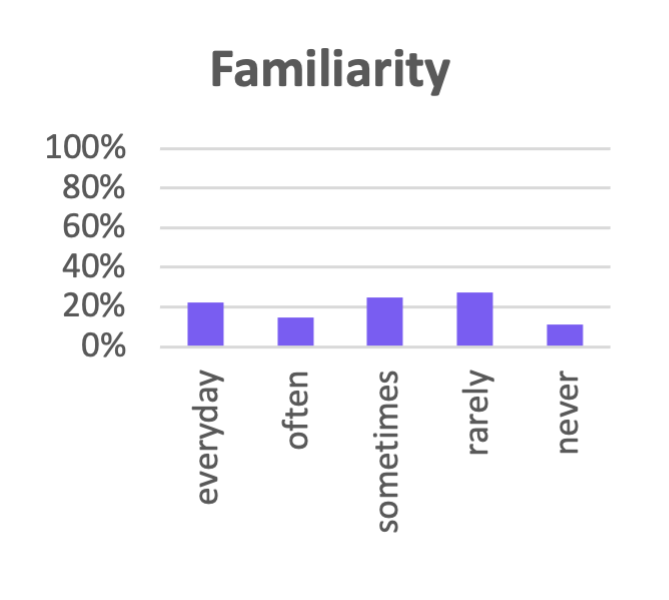
\includegraphics[width=\w]{figures/familiarity_distribution.png}\hfill
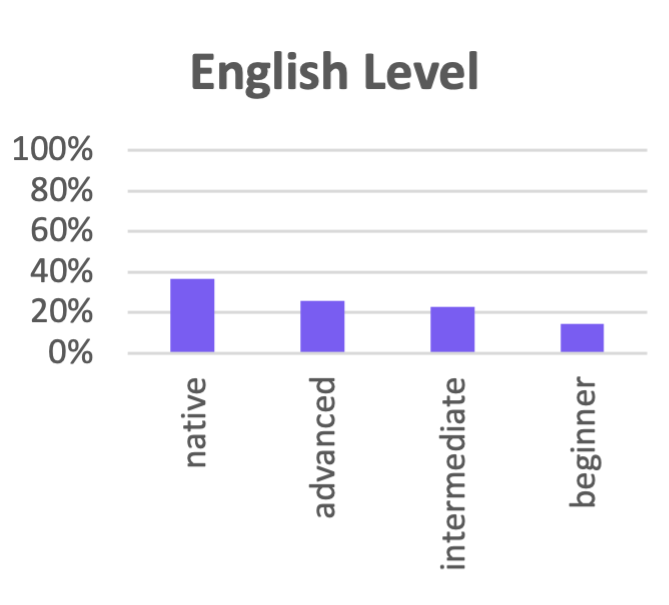
\includegraphics[width=\w]{figures/english_distribution.png}\hfill
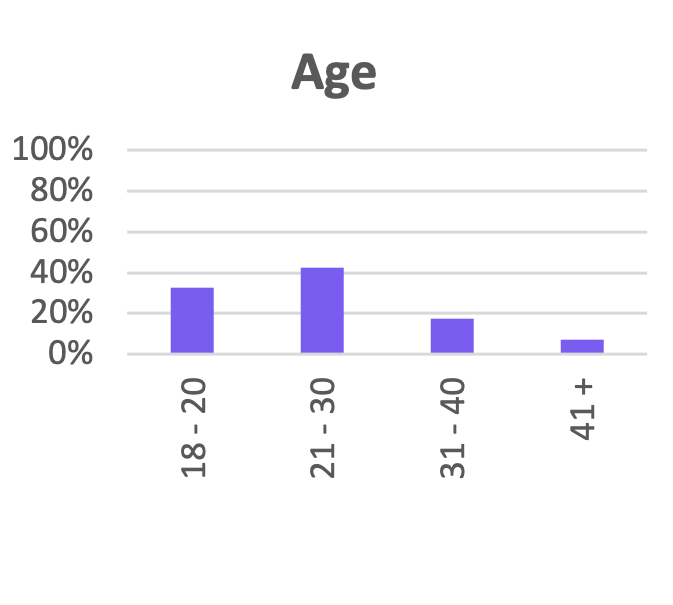
\includegraphics[width=\w]{figures/age_distribution.png}\hfill
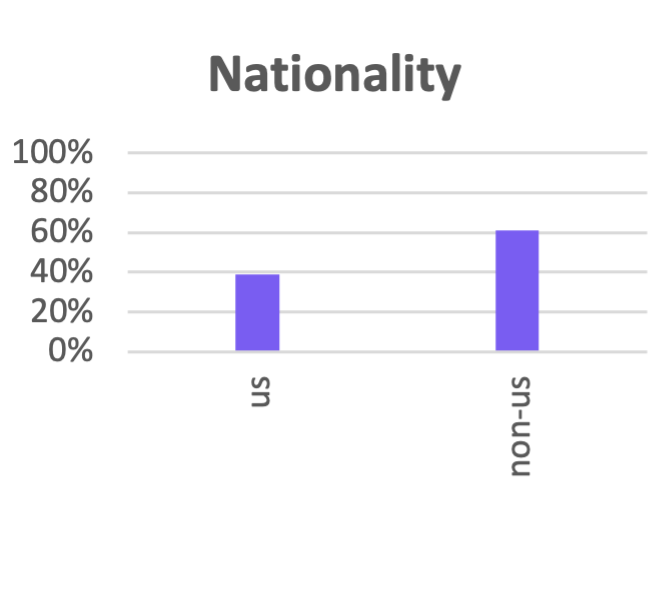
\includegraphics[width=\w]{figures/nat_distribution.png}\\
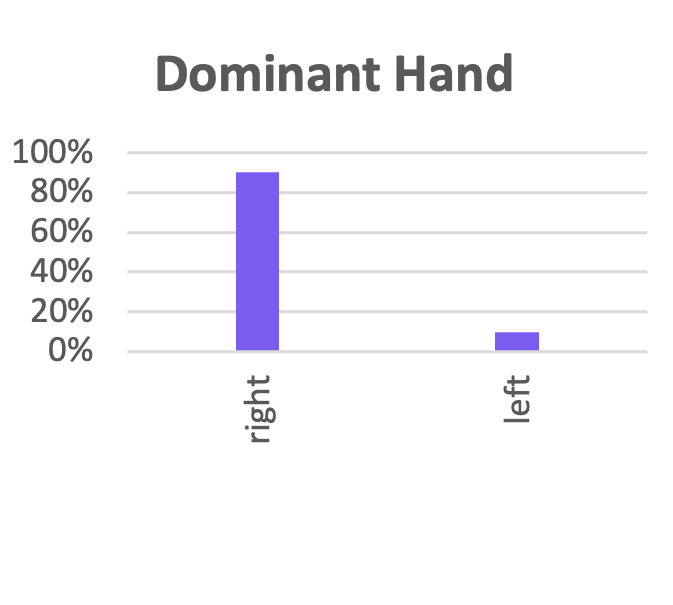
\includegraphics[width=\w]{figures/dom_distribution.png}\hfill
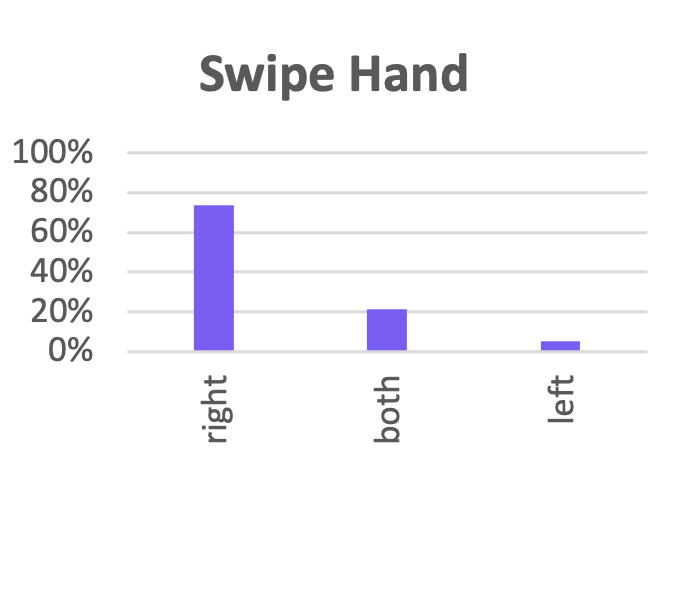
\includegraphics[width=\w]{figures/hand_distribution.png}\hfill
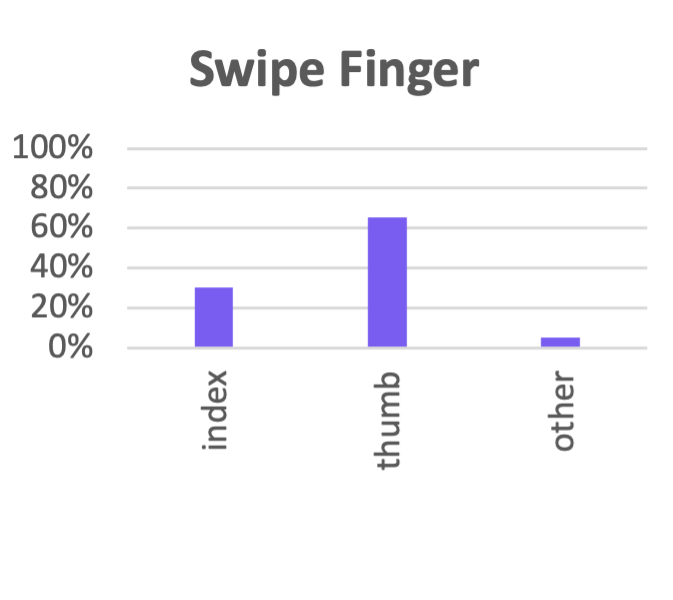
\includegraphics[width=\w]{figures/finger_distribution.png}\hfill
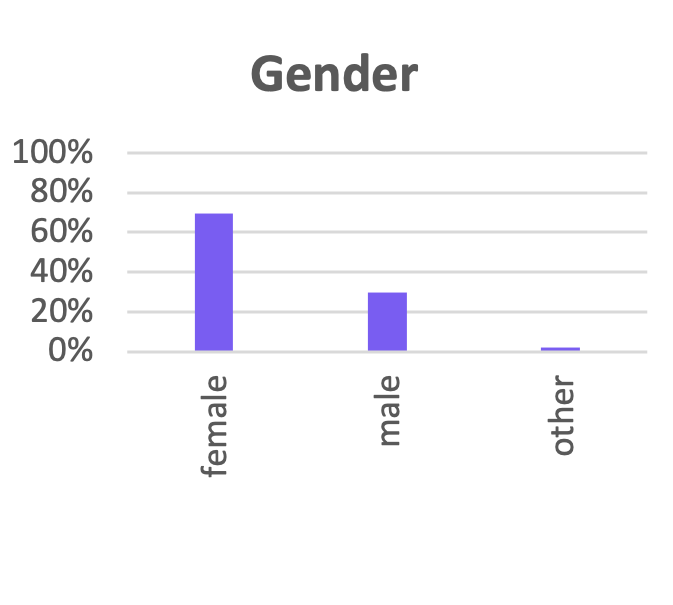
\includegraphics[width=\w]{figures/gender_distribution.png}\\
\caption{Targets and their class distributions in \%}\label{fig:distributions}
\end{figure}

In \autoref{fig:distributions}, the class distributions of the targets are shown. From the figures we can see that some targets are imbalanced in their class distributions than others. This can potentially introduce a bias to our model training. To address this challenge we employed different techniques. In the following paragraphs, we explain and analyze the targets and their class distributions in more details.\\

%For instance, considering a binary classification where the minority class is underrepresented relative to a majority class. The model will then adjust its weights during training such that the number of classification errors is minimized w.r.t. the majority class and the minority class is largely ignored. The total cost remains low even if the model mostly misclassifies the instances of the minority class due to their little occurrences during training. On the other hand, the total cost remains high when the number of misclassifications in the majority class is high due to their very frequently occurrences during training. Thus, the model often decides in such an imbalance situation to classify the most data instances of the majority class. The resulting accuracy will be high regardless of whether the instances of the minority class are properly classified.

The familiarity label describes how well a user is used to swiping and contains 5 classes namely everyday, often, sometimes, rarely and never. By looking at the class distributions, we can see that the class never accounts for 11\%, while rarely accounts for 27\%, sometimes for 25\%, everyday for 22\% and often for 15\%. In order to balance the slight imbalances here, we merged the class everyday with often as well as the class rarely with never; by doing so we end up with 3 classes accounting for 37\%, 25\% and 38\% of the distribution.
The English level target has 4 classes namely native, advanced, intermediate and beginner, accounting for 37\%, 26\%, 23\% and  14\% of the class distribution respectively.  For the age target, we have 4 initial classes i.e., youth(18-20 years), young(21-30 years), adult(31-40 years) and senior(41+ years). By looking at the class distributions for age, we have 33\% youth, 42\% young, 18\% adult and 7\% senior. \autoref{fig:age-seq} further illustrates the distributions for every existing age in the metadata and we can see that people older than 60 years can be considered outliers. Hence, we decided to have 3 classes i.e., youth(18-20 years), young(21-28 years) and adult(29+ years) accounting for 33\%, 37\%  and 30\% of the class distribution.\\

\begin{figure*}[h]
    \centering
    \def\w{0.45\textwidth}
    \subfloat[\text{Age}]{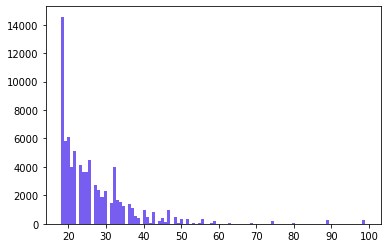
\includegraphics[width=\w]{figures/age.png}}
    \hspace{1cm}
    \subfloat[\text{Sequence Length}]{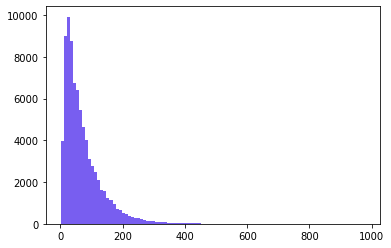
\includegraphics[width=\w]{figures/sequence_length.png}}
    \caption{Distributions for age and sequence length}
    \label{fig:age-seq}
\end{figure*}\\

The nationality label describes if a user is a US or non-US citizen. In the metadata 39\% of the users are US  and the remaining 61\% are non-US. The dominant hand label describes if the user's dominant hand is right or left. The distribution of the two classes are  90\%  right handed and 10\% left handed. The swipe hand label describes if the user likes to use the right, left or both hands to swipe. By looking at the class distributions for swipe hand, we have  3 classes 74\% right hand, 21\% both hands and 5\% left hand. Due to their significant difference in size compared to the right hand, we decided to merge the classes left and both. Consequently, we end up with 2 classes accounting for 74\% and 26\%. The swipe finger label describes which finger the user prefers to swipe with. We have 3 different classes, index, thumb and other accounting for 65\% , 30\% and  5\% of the class distributions respectively.  We left out the class `other' due to its insignificance in size such that we only have 2 classes with 69\% and 31\%. For the gender label we have 69\% female, 30\% male and 1\% other. Similarly we left out the class `other' due to its insignificance in size such that we only have 2 classes with 70\% and 30\%. The targets nationality, dominant hand, swipe hand, swipe finger and gender have a significant imbalance in their class distributions. The details on how we further addressed the class imbalance issue will be discussed in the next section.\\

For the data split ratio, we used 60\% for the training set, 20\% for the validation set and 20\% for the testing set. In \autoref{fig:age-seq}, the distributions of the sequence lengths are shown and we can observe that most of the trajectories have a sequence length between 1 and 200. Neural networks require inputs with the same shape and size. Thus, we needed to apply padding to our sequence trajectories since all the sequences do not have the same length. We chose 200 as our maximum length. All sequences are padded or truncated to this maximum capacity. \newpage

\section{Methodology}

%% What models were selected? Diagram of the architectures: input layer -> recurrent layer(s) -> dropout -> dense layer -> output layer
%% What are their characteristics? Who do they work? Add diagrams of RNN/LSTM/GRU cells.
%% What hyperparameters were varied? e.g. num hidden layers, num hidden units, etc.
%% How the models were trained? optimizer (Adam), batch size, early stopping, etc.

Swipe trajectories are sequences of coordinates, thus for  the task of predicting user demographics from swiping behaviour we have chosen to train sequence models.  Sequence models are machine learning models better suited to handle sequential data  where each observation is dependent or contextually related to the previous one such as text streams, audio clips, trajectories, time-series data, etc. Recurrent Neural Network (RNN) is a popular algorithm used in sequence models. RNN models consist of standard recurrent cells, shown in \autoref{fig:rnn-model}.\\

The typical feature of the RNN cell is a cyclic (or \emph{loop}) connection,
which enables the model to update the current state based on past states and current input data.
Formally, the standard recurrent cell is defined as follows:
%
\begin{align}\label{eq:rnn}
    h_j &= \Phi(W_h h_{j-1} + W_z z_j + b) \\
    o_j &= h_j
\end{align}
%
where
%
$z_j = (x,y,t)_j$ denotes the $j$th vector of the input signal
$\mathbf{z} = (x,y,t)_{j = 1, \cdots, |z|}$ at timestep $j$
(i.e., the index at which a point coordinate has happened),
$h_j$ is the hidden state of the cell,
and $o_j$ denotes the cell output, respectively;
$W_h$ and $W_z$ are the weight matrices;
$b$ is the bias of the neurons;
and $\Phi$ is an activation function.

\begin{figure}[!ht]
\centering
\centerline{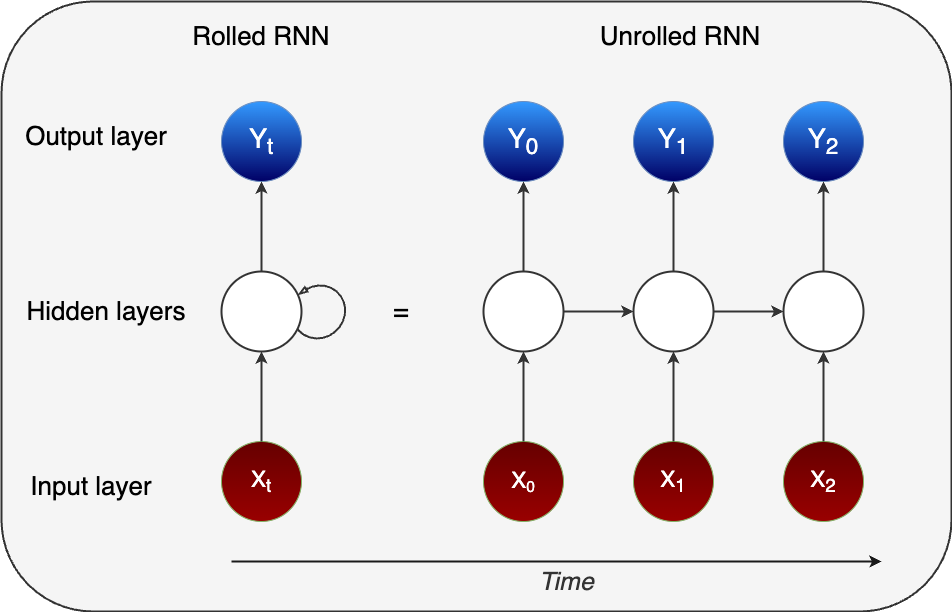
\includegraphics[width= 0.55\linewidth]{plots/RNN.png}}
\caption{Standard RNN}
\label{fig:rnn-model}
\end{figure}
Standard recurrent cells have achieved success in many sequence learning problems
such as natural language processing~\cite{Sutskever14}, action recognition~\cite{Du18}, or image captioning~\cite{Mao15}.
However, the standard recurrent cells are not capable of handling long-term dependencies.
To solve this issue, the LSTM and GRU cells were developed~\cite{Hochreiter97_lstm, Cho14_gru}.
They improve the capacity of the standard recurrent cell by introducing different gates,
which we briefly describe as follows.\\

On the one hand, the LSTM cell is defined as follows:
%
\begin{align}\label{eq:lstm}
        G_i &= \sigma(W_u [ h_{j-1}, z_j ] + b_i) \\
        G_f &= \sigma(W_f [ h_{j-1}, z_j ] + b_f) \\
        G_o &= \sigma(W_o [ h_{j-1}, z_j ] + b_o) \\
        c_j &= G_u \odot \tilde{c}_j + G_f \odot c_{j-1} \\
\tilde{c}_j &= \Psi(W_c [ h_{j-1}, z_j ] + b_c) \\
        h_j &= G_o \odot \Psi(c_j)
\end{align}
%
where
    $c_j$ is an additional hidden state, % cell state: long-term memory
$W_*$ are weight matrices,
$b_*$ are biases,
$G_*$ denote cell gates (i: input, f: forget, o: output, u: update),
and $\Psi$ and $\sigma$ are activation functions (hyperbolic tangent and sigmoid, respectively).
The $\odot$ operator denotes the Hadamard (element-wise) product.\\

As noted, the LSTM has two kinds of hidden states~\cite{Jozefowicz15}:
a ``slow'' state $c_j$ that keeps long-term memory, % to overcome the vanishing gradient problem,
and a ``fast'' state $h_j$ that makes decisions over short periods of time.
The forget gate can decide what information will be thrown away from the cell state.
In practice, the activation functions $\Psi$ and $\sigma$ are hyperbolic tangent and sigmoid, respectively,
however other non-linear functions have been promoted in the research literature;
see next section for a brief discussion.\\

On the other hand, the GRU cell is defined as follows:
%
\begin{align}\label{eq:gru}
        G_u &= \sigma(W_u [ h_{j-1}, z_j ] + b_u) \\
        G_r &= \sigma(W_r [ h_{j-1}, z_j ] + b_r) \\
\tilde{c}_j &= \Psi(W_c [G_r \odot h_{j-1}, z_j ] + b_c) \\
        h_j &= G_u \odot \tilde{c}_j + (1 - G_u) \odot h_{j-1}
\end{align}
%
where the forget and input gates of the LSTM cell are now combined into a single update gate $G_u$.
A reset gate $G_r$ controls which parts of the state get used to compute next cell state. The LSTM and GRU architectures are presented in figure \autoref{fig:LSTM_GRU model}.\\

\begin{figure}
     \centering
     \begin{subfigure}[b]{0.45\textwidth}
         \centering
         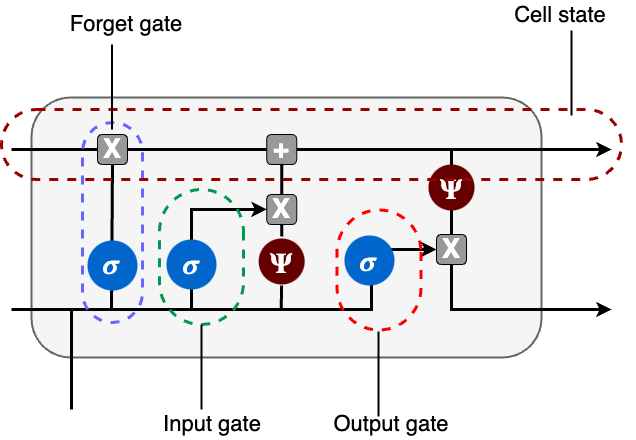
\includegraphics[width=\textwidth]{plots/LSTM.png}
         \caption{LSTM}
         \label{fig:lstm-model}
     \end{subfigure}
     \hspace{1cm}
     \begin{subfigure}[b]{0.45\textwidth}
         \centering
         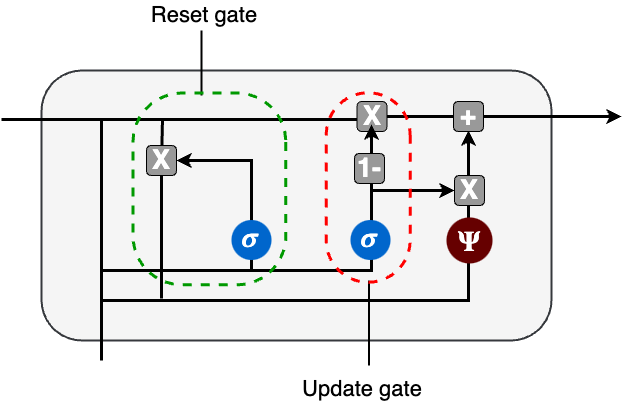
\includegraphics[width=\textwidth]{plots/GRU.png}
         \caption{GRU}
         \label{fig:gru-model}
     \end{subfigure}
    \caption{LSTM and GRU architectures}
    \label{fig:LSTM_GRU model}
\end{figure}

As can be observed, GRU controls the flow of information like the LSTM cell,
but without having to use memory (the forget and output gates in LSTM):
the full state vector is output at every time step.
Furthermore, performance-wise the GRU cell has been shown to be on par with the LSTM in many problems~\cite{Chung14,Dey17}
while at the same time being computationally more efficient because of its less complex structure.
It remains unclear, however, what would be the best RNN-based architecture configuration
(e.g. type of cell, number of layers, number of neurons, etc.)
for predicting biometric and behavioral traits traits from swipe trajectories.
Therefore, we study what is the most suitable configuration.\\

The classification rule of all the classifiers we examined in this paper is defined by:
\begin{equation}\label{eq:classification-rule}
\hat{z} = \text{softmax}(W_z \odot h_j + b_z)
\end{equation}
%
where $\text{softmax}(\mathbf{v})$ is the softmax function,
which normalizes the output of the last network layer
(denoted as $\mathbf{v}$ for the sake of simplicity)
to a probability distribution over the predicted output classes $K$:
%
\begin{equation}\label{eq:output}
  \text{softmax} ( \mathbf{v} )_{i} = \frac{e^{v_i}}{\sum _{j=1}^{K} e^{v_j}}
\end{equation}
%
for $i = \{1, \dots, K\}$ and $\mathbf{v} = (v_1, \dots, v_K)$. \\

We chose to do a systematical analysis about how the change of popular architecture hyperparameters of our model might affect the model's performance metrics. The popular architecture choices are the type of layer(RNN, LSTM or GRU), if bidirectional or not, the number of hidden neurons, the number of hidden layers and the learning rate. \\

Bidirectional models(BiRNN, BiLSTM, BiGRU) are recurrent neural networks, where the input flows in both directions such that every component of an input sequence is able to use the information from both the past and present. The model adds for each recurrent layer another recurrent layer with the reversed information flow. The outputs from forward and backward layers are combined by default with the concatenation in Keras. The disadvantage of bidirectional models is that they are slower since they require more time for training. Firstly, we tested the performance of the different types of models RNN, BiRNN, LSTM, BiLSTM, GRU and BiGRU for each target.\\

We tested how the number of hidden layers as well as the number of hidden neurons impacts our model's performance. The hidden layer variations are from 1 to 4 recurrent hidden layers in our model's architecture. The hidden units variations are from 10 to 150 neurons with a step size of 10. We used a dropout with the probability of 0.15 in all layers. The hyperbolic tangent activation function is applied in every recurrent layer since recurrent neural networks do not only get gradients from lower layers but also from previous timesteps. The derivatives of tanh are larger than the ones of the sigmoid activation function. Thus, the cost function is minimized faster by using the hyperbolic tangent activation function. It has a normalized range from -1 to 1 and the output is symmetric around 0 which leads to faster convergence. Formally:
\begin{equation}\label{eq:tanh}
  \text{tanh(z)} = \frac{e^{z} - e^{-z} }{e^{z} + e^{-z} }
\end{equation}\\

The learning rate controls how quickly a neural network model adapts to a problem. By choosing smaller learning rates, the model might result in a long training or might get stuck in the process since the changes made to the weights each update are smaller. On the other hand, the model might converge too fast to a sub-optimal solution by choosing larger learning rates. We chose to use the learning rates 10$^{-1}$, 10$^{-2}$, 10$^{-3}$, 10$^{-4}$ and 10$^{-5}$. For the optimizer we chose to work with the Adam optimizer since it is an algorithm for efficient stochastic optimization that only requires first-order gradients with little memory requirement~\cite{Adam}. The loss function to minimize is sparse categorical cross-entropy, since our task is a multi-class classification problem.\\

%%%While training, the model underfits if we train the model too little. On the other hand, the model overfits the train set and perfoms poorly on the test set if we train too long.  We decided therefore to apply early stopping in the training of our neural network. Thus, our model trains on the train set until its performance on the validation set starts to degrade i.e. generalization error starts to increase.

We chose F1 score as one of our model performance evaluation mercies since it is a popular metric for imbalanced classification problems. The F1 score, \autoref{eq:fscore} is the harmonic mean of precision and recall. Precision, \autoref{eq:precision} is the ratio of correctly predicted positive instances True positives(TP) divided by the total number of predicted positive instances both True and False Positives (FP). The recall, \autoref{eq:recall} identifies the number of correct positive predictions among all positive predictions that were possible TP and False Negatives(FN).

%The batch size is the number of samples that are processed before the internal model parameters are updated. A model will finish faster at each epoch during training if the batch size is larger since it depends on the computational resources. On the other hand, the model's quality might decrease when the batch size increases and the model might not generalize well unseen data. We set therefore our batch size to 32.

\begin{equation}\label{eq:precision}
    \text{Precision} = \frac{\text{TP}}{\text{TP} + \text{FP}}
\end{equation}
\begin{equation}\label{eq:recall}
    \text{Recall} = \frac{\text{TP}}{\text{TP} + \text{FN}}
\end{equation}
\begin{equation}\label{eq:fscore}
    \text{F-Score}=  \frac{2 \cdot \text{Precision} \cdot \text{Recall}}{\text{Precision} + \text{Recall}}
\end{equation}\\

In all experiments we set the patience value to 40 epochs(early stopping), the maximum number of training epochs to 500 epochs and batch size to 32.\\

As discussed in section 3.1, we have imbalances in the class distributions of the different targets. To address this challenge we used cost-sensitive models. The idea is to give all the classes equal importance on gradient updates, on average, regardless of how many samples we have from each class in the training data. This prevents models from predicting the more frequent class more often just because it’s more common. Instead, class weighting pushes models to learn a better representation of each class. In particular we used the sklearn utility function to compute the appropriate class weights in our training.\newpage

%%%to assign different weights to different misclassification errors. More precisely, we want to force the model to pay more attention to the minority classes during training by making the weight of misclassification relatively high compared to the weight of misclassification in the majority class. Thus, the classifier learns then similarly from minority and majority classes and the class weights regularize the loss function. The model has a higher loss due to the misclassification of the minority classes. The model is forced to learn representations for the minority classes and the performance for the majority class is slightly reduced. We used the sklearn utility function to compute the appropriate class weights.


\section{Experimental Setup}

For the experiments, we defined sequence models with different architectural hyperparameters choices. The sequence models are well-known to have long training times. Thus, we decided to run almost all our models with the Uni.lu High Performance Computing(ULHPC)\footnote{\url{https://hpc-docs.uni.lu}}, which allows us to achieve high-quality results in our deep learning tasks. We defined a bash script that helped us to reserve and allocate resources for the execution of our scheduled jobs. We worked with the iris cluster, which is a Dell/Intel supercomputer. It offers a theoretical peak performance of 1082 TFlop/s and features 196 computing nodes, 5824 computing cores and 96 GPU accelerators\footnote{\url{https://hpc-docs.uni.lu/systems/iris/}}.\\


\begin{figure}[!ht]
\centering
\centerline{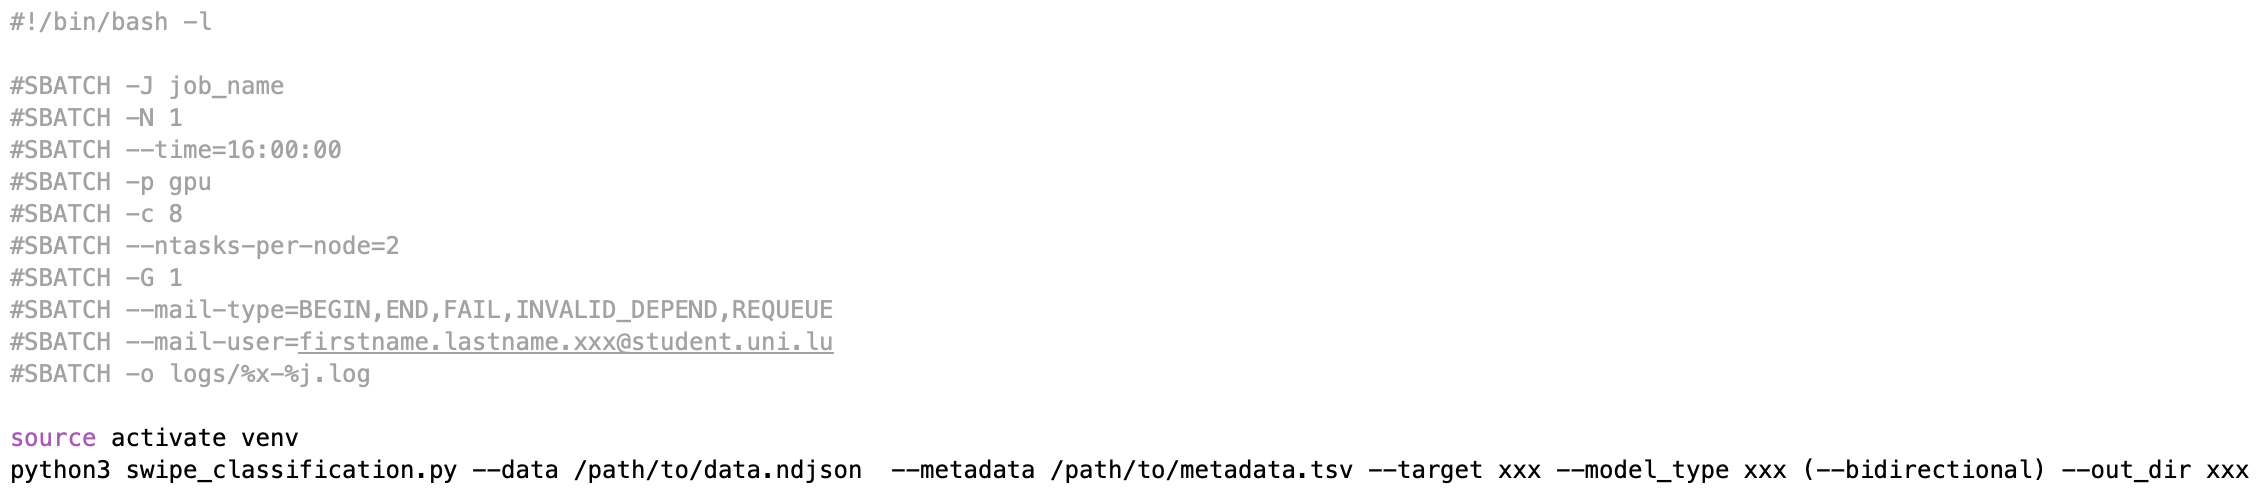
\includegraphics[width=1\linewidth, frame]{figures/bash_script.png}}
\caption{HPC - Job Launcher Script}
\label{fig:launcher_script}
\end{figure}

We submitted passive jobs for our different executions of the models i.e. we used sbatch to submit our job launcher script for later execution. In ~\autoref{fig:launcher_script}, our job submission options are shown\footnote{\url{https://hpc-docs.uni.lu/slurm/}}. We defined for each job its name and requested 1 GPU node with 768 GB of RAM. We requested 8 cores per task and 2 tasks per node.  We set the walltime to different times since for bidirectional models we assured to have even more time available than for non-bidirectional ones. We got notifications by email when specific events occured e.g. the job begins, fails, ends, etc. such that we looked at the log files with the results after the execution ended. In ~\autoref{table:cli}, the different kind of arguments are listed for our CLI parser. We defined this parser to be able to ease the way of defining the chosen architectural hyperparameters and submitting the jobs to HPC. It was required to at least define always the model type e.g. RNN, GRU or LSTM, if the model is bidirectional, the output directory and the demographical target about which the model should learn and predict. In our experiments, we changed only the values of the learning rate argument from 10$^{-1}$ to 10$^{-5}$, the units argument from 10 to 150, and the hidden layers from 1 to 4. For most of the parser arguments, we defined default values since there was no need to touch them. The eval\textunderscore model argument was useful if somehow we wanted just to evaluate a given model that was already trained before.\\

We experimented by training more than 200 different recurrent neural networks in total since our models predicted on 8 demographical traits with approximately 27 different hyperparameter variations for each target. Each network trained for at least 40 epochs. A model took a lot of time in training e.g. for a non-bidirectional model from at least 1,5 to 10 hours and for a bidirectional model from at least 3 to 20 hours, since the nature of the models were recurrent and the hyperparameter choices affected the training time. Firstly, we always tested in our experiments which model architecture, e.g. RNN, BiRNN, GRU, BiGRU, LSTM and BiLSTM, performed best. We conducted for 5 features 21 experiments with  either a bidirectional LSTM or GRU model, i.e. very long training times due to the model type choices already.\\


\begin{table}[h]
\resizebox{\linewidth}{!}{
\centering
\begin{tabular}{||c|c|c||}
 \hline
 Argument & Description & Default\\
 \hline
  data & path to data.ndjson & required\\ \hline
  data & path to data.ndjson & required\\ \hline
  model\textunderscore type & {rnn, lstm, gru} & required\\ \hline
  target & dominant\textunderscore hand, swipe\textunderscore finger, swipe\textunderscore  hand, gender, nationality, english\textunderscore level, familiarity, age & required \\ \hline
  out\textunderscore dir & path to write model & required \\ \hline
  bidirectional & use bidirectional cells & false \\ \hline
  layers & number of hidden layers & 2 \\ \hline
  units & dimensionality of output embedding & 100 \\ \hline
  lr & learning rate & 0.0001 \\ \hline
  epochs & number of training epochs & 500 \\ \hline
  patience & number of consecutive epochs without improvement to stop training & 40 \\ \hline
  batch size & training batch size & 32 \\ \hline
  drop\textunderscore out & dropout value & 0.15 \\ \hline
  max\textunderscore length & max number of timesteps & 200 \\ \hline
  training\textunderscore split & training partition size & 0.8 \\ \hline
  validation\textunderscore split & validation partition size, relative to training partition & 0.2 \\ \hline
  testing\textunderscore split & testing partition size & 0.2 \\ \hline
  activation & activation function in hidden layers & tanh \\ \hline
  eval\textunderscore model & path to model file, for evaluation &  \\ \hline
  workers & number of workers to parallelize training & 8 \\ \hline
  verbose & display more information to stdout & 2 \\ \hline
 \hline
\end{tabular}}
\caption{CLI Parser Arguments}
\label{table:cli}
\end{table}

We used occasionally also Google Colab Pro+ when the HPC was on maintenance or if the nodes were too busy such that our jobs remained some days in the queue e.g high demand of job execution requests or when other bigger jobs with a walltime of 3-5 days reserved the nodes. Colab Pro+ permitted us access to GPUs or TPUs depending their availability. It offers system RAM up to 52GB, GPU RAM of 16GB, more stability in your connection than Colab and the background execution option that allows continuous code execution for up to 24 hours.\newpage



\chapter{Results and Discussion}
\addcontentsline{lof}{chapter}{Results and Discussion}
\addcontentsline{lot}{chapter}{Results and Discussion}

%% Plots: Accuracy, AUC, F1

%% TODO: Improve the look and feel of the plots:
%% - Remove outer gray border from main plot and legend.
%% - Enlarge the X axis label (e.g. "model architecture") and use a bold font.
%% - Use a more accesible color palette: https://davidmathlogic.com/colorblind/#%23D81B60-%231E88E5-%23FFC107-%23004D40
%% - Add plot titles, indicating the number of classes; e.g. "Familiarity (5 classes)".
%% - Draw a horizontal black line denoting random classification; e.g. for 2 clases it would be a line at Y=50%.

In this section we present results obtained from our experimental evaluations. Due to the class imbalance issue in the dataset, classification accuracy is not sufficient as indicator to evaluate the performance of our classifiers. Hence, we also report the F1 score as well as the Area Under the ROC curve (AUC) that determines the discriminatory power of a classifier. We report the accuracy of a random classifier as our baseline (horizontal black dotted line) in the plots, for which we compute the \emph{a priori} distribution of the number of classes $C$:
\begin{equation}
    \text{Random Accuracy (\%)} = \frac{100}{C}
\end{equation}\\

In our experiments we have investigated how the model's performance metrics change by manipulating the different hyperparameters (i.e., model type(RNN, GRU, LSTM), if bidirectional or not, the number of hidden layers and hidden units as well as the learning rate.) The best performance results obtained through a systematic analysis of the chosen hyperparameters in classifying user demographics from swiping trajectories  are reported  with the plots per target from \autoref{fig:fam} to \autoref{fig:finger}. In \autoref{appendix:app_fam} - \autoref{appendix:app_finger}, all the intermediate experiments results can be found in tables.\\

For the swiping familiarity target \autoref{fig:fam}, with 3 classes, a random classifier's accuracy is 33,33\%.  The best performance accuracy achieved in our experiments is 37,87\%  with a the configuration: LSTM, 2 hidden layers, 140 hidden units and a learning rate of 10$^{-4}$.\\

For the English level target \autoref{fig:engl}, with 4 classes, a random classifier's accuracy is 25\%. The best performance accuracy achieved in our experiments is 37,32\% with the configuration: BiLSTM , 4 hidden layers, 100 hidden units and a learning rate of 10$^{-4}$.\\

For the Age target \autoref{fig:age}, with 3 classes the accuracy of a random classifier is 33,33\% . Whereas,  the best performance accuracy achieved in our experiments is 40,91\% with the configuration: BiGRU, 2 hidden layers, 150 hidden units and a learning rate of 10$^{-3}$. \\

For the nationality target \autoref{fig:nat}, with 2 classes a random classifier's accuracy is 50\%. Whereas, the best performance accuracy achieved in our experiments is 63,50\% with the configuration: RNN, 2 hidden layers, 150 hidden units and a learning rate of 10$^{-4}$. \\

For the gender target in \autoref{fig:gender}, with 2 classes a random classifier's accuracy is 50\%. The best performance accuracy achieved in our experiments is 68,51\% with the configuration BiLSTM model, 2 hidden layers, 50 hidden units and a learning rate of 10$^{-1}$.\\

For the dominant hand target in \autoref{fig:dom}, with 2 classes the accuracy of a random classifier is 50\%. The best performance accuracy achieved in our experiments is 88,57\% with  the configuration BiLSTM model, 2 hidden layers, 150 hidden units and a learning rate of 10$^{-2}$.\\

For the swiping hand target in \autoref{fig:hand}, with 2 classes a random classifier's accuracy is 50\%. The best performance accuracy achieved in our experiments is 58,74\% with the configuration: LSTM model, 2 hidden layers, 100 hidden units and a learning rate of 10$^{-3}$.\\

For the swiping finger target in \autoref{fig:finger}, with 2 classes a random classifier's accuracy is 50\%. The best performance accuracy achieved in our experiments is 69,28\% with the configuration: GRU model, 2 hidden layers, 100 hidden units and a learning rate of 10$^{-1}$.\\

\begin{figure}[h]
     \centering
     \def\w{0.4\linewidth}
     \begin{subfigure}{\w}
         \centering
         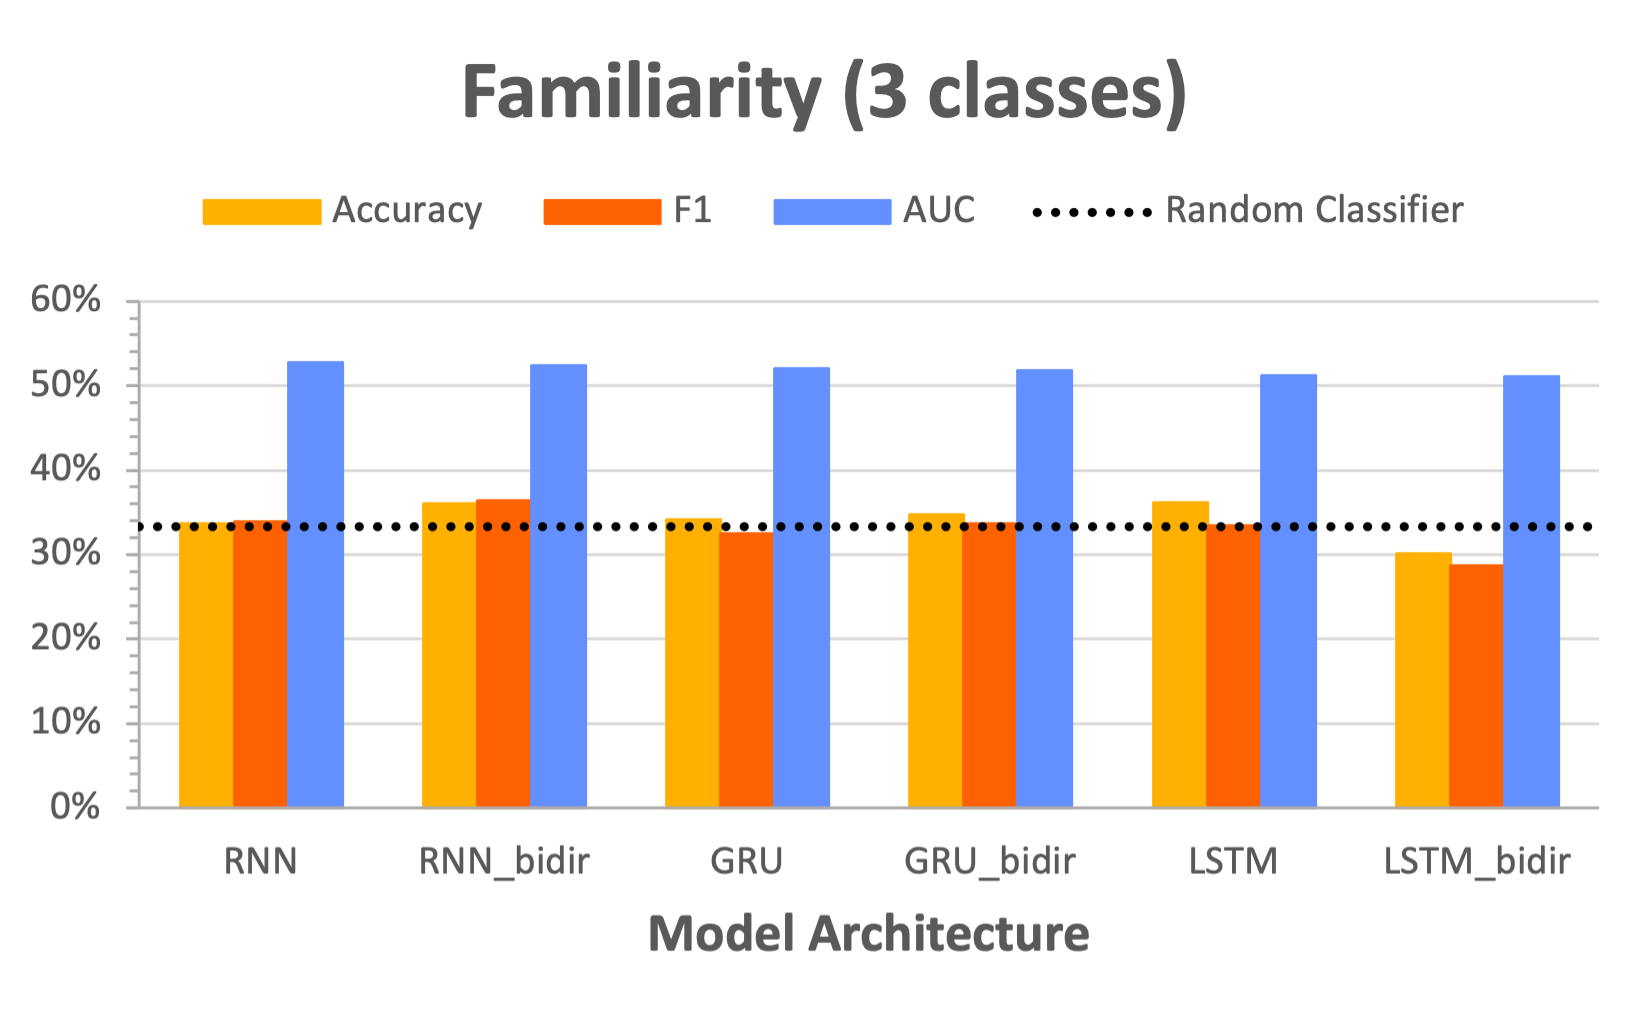
\includegraphics[width=\textwidth]{plots/model_fam.png}
         \caption{Classifiers}
         \label{fig:models_fam}
     \end{subfigure}
     \hfill
     \begin{subfigure}{\w}
         \centering
         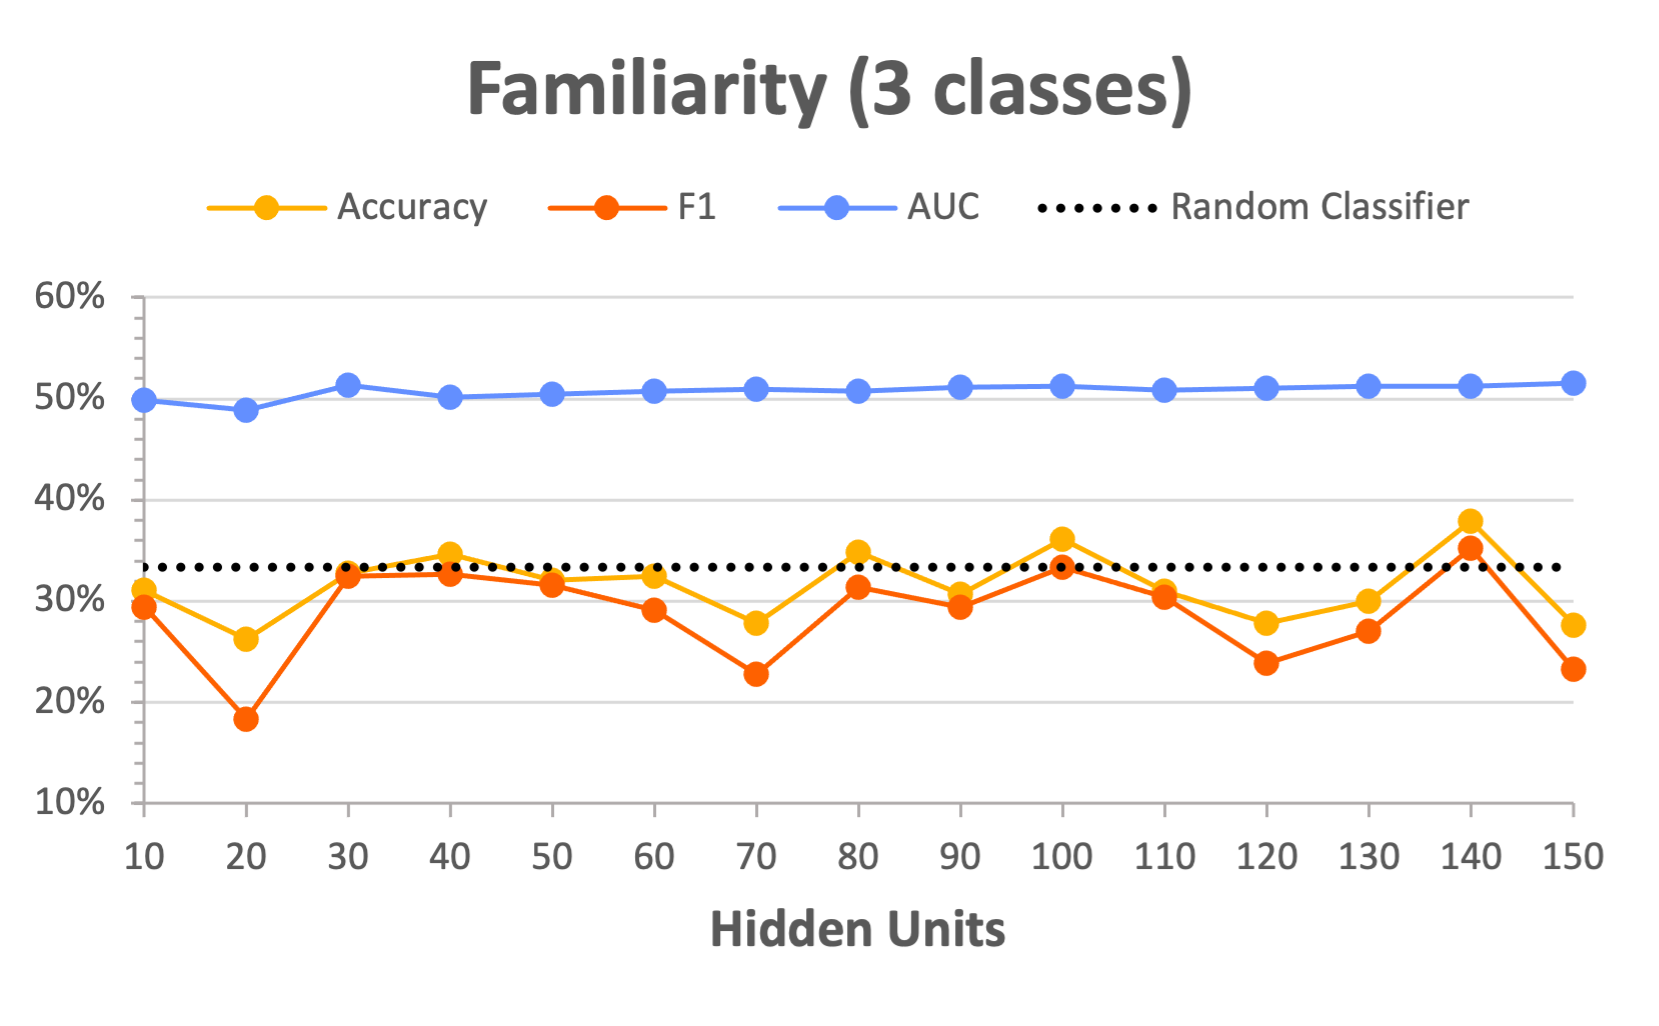
\includegraphics[width=\textwidth]{plots/units_fam.png}
         \caption{Hidden Units}
         \label{fig:units_fam}
     \end{subfigure}\\
     \begin{subfigure}{\w}
         \centering
         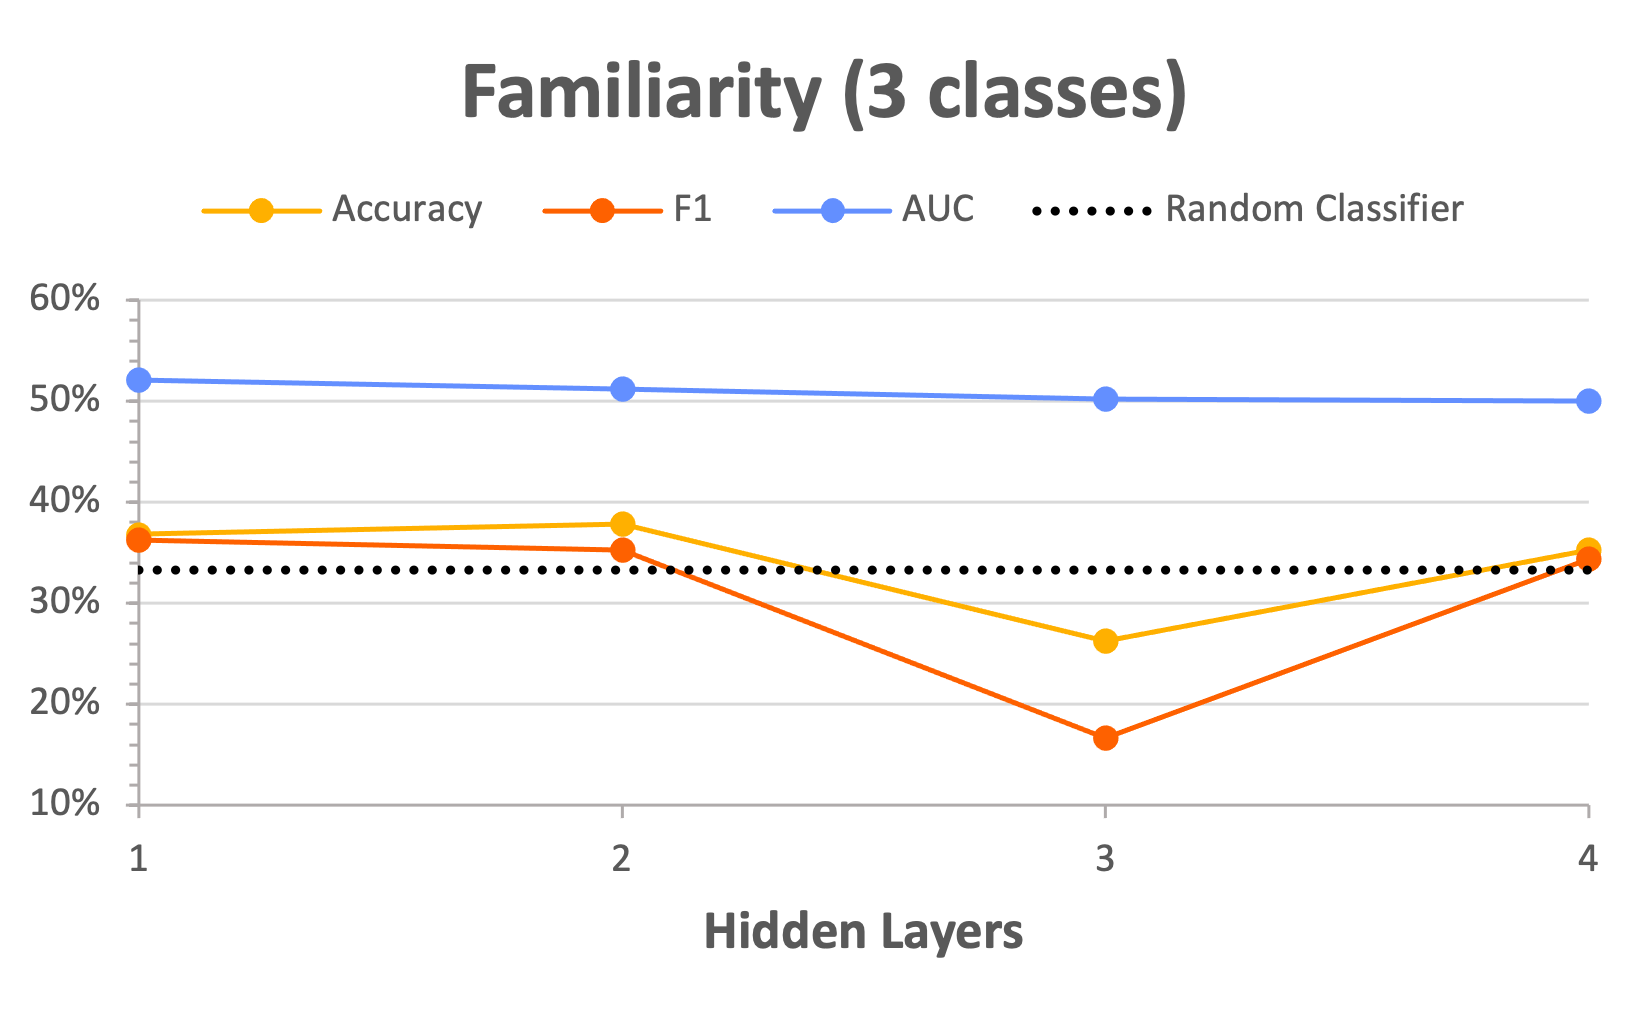
\includegraphics[width=\textwidth]{plots/layers_fam.png}
         \caption{Hidden Layers}
         \label{fig:layers_fam}
     \end{subfigure}
     \hfill
     \begin{subfigure}{\w}
         \centering
         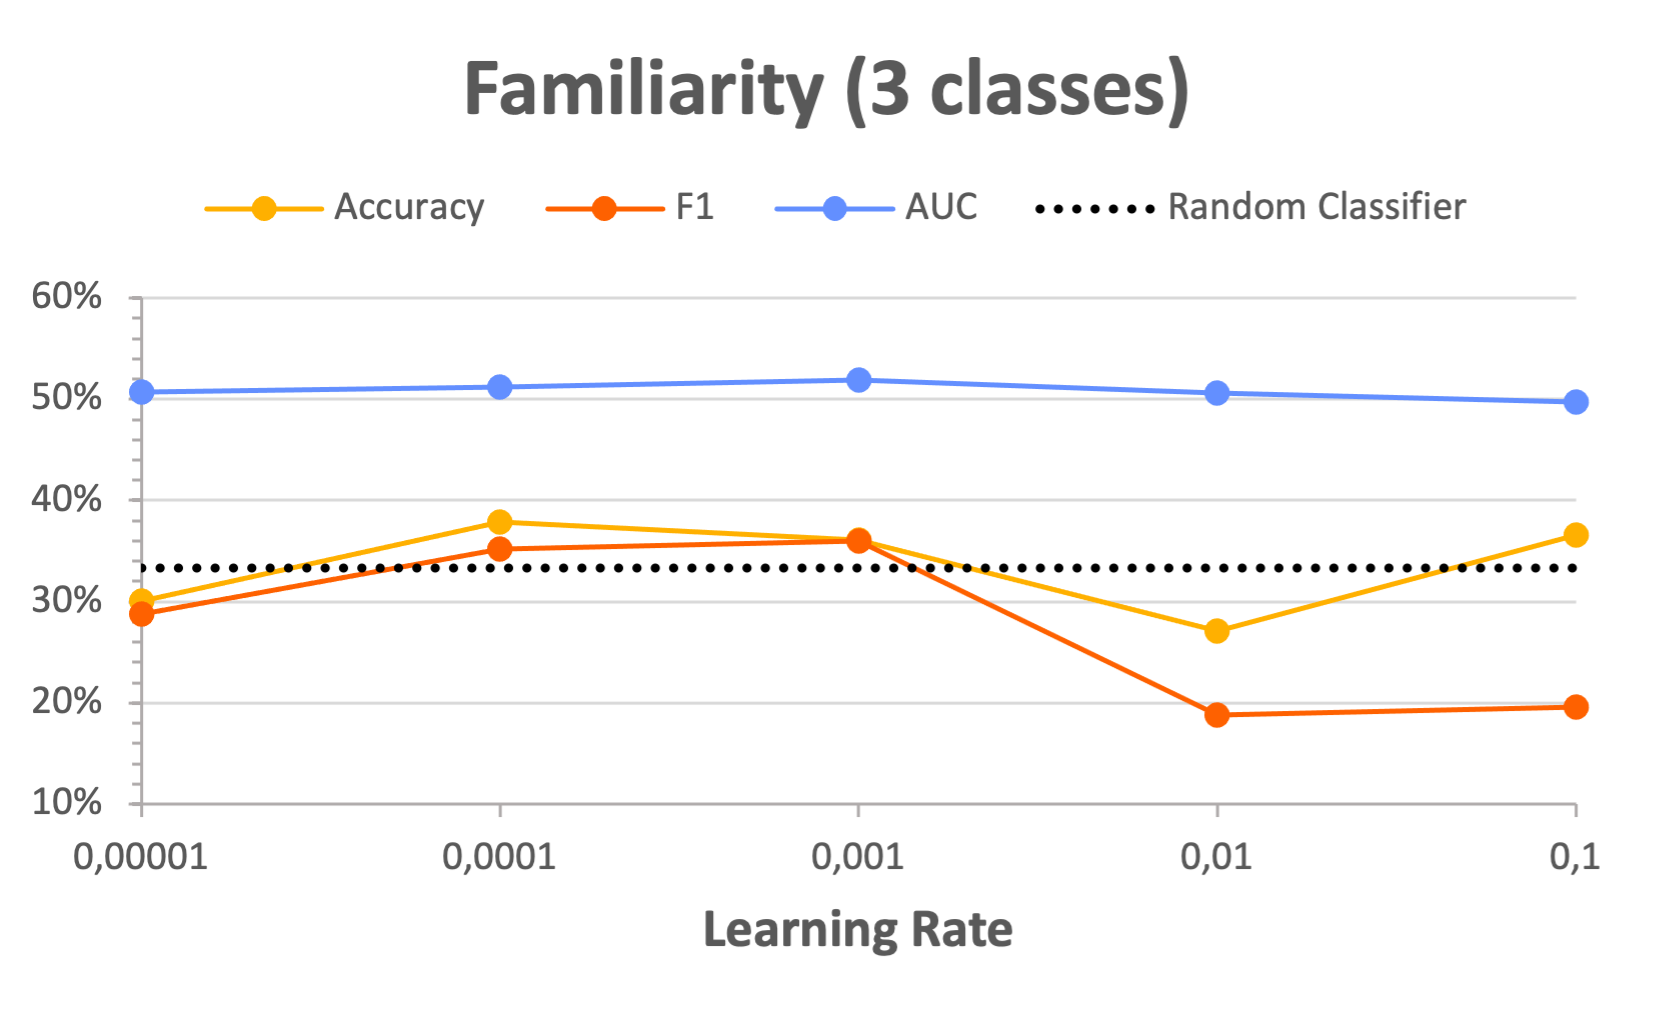
\includegraphics[width=\textwidth]{plots/lr_fam.png}
         \caption{Learning Rate}
         \label{fig:lr_fam}
     \end{subfigure}

    \caption{Familiarity - Experiment Results}
    \label{fig:fam}
\end{figure}
\begin{figure}[]
     \centering
     \def\w{0.45\linewidth}
     \begin{subfigure}{\w}
         \centering
         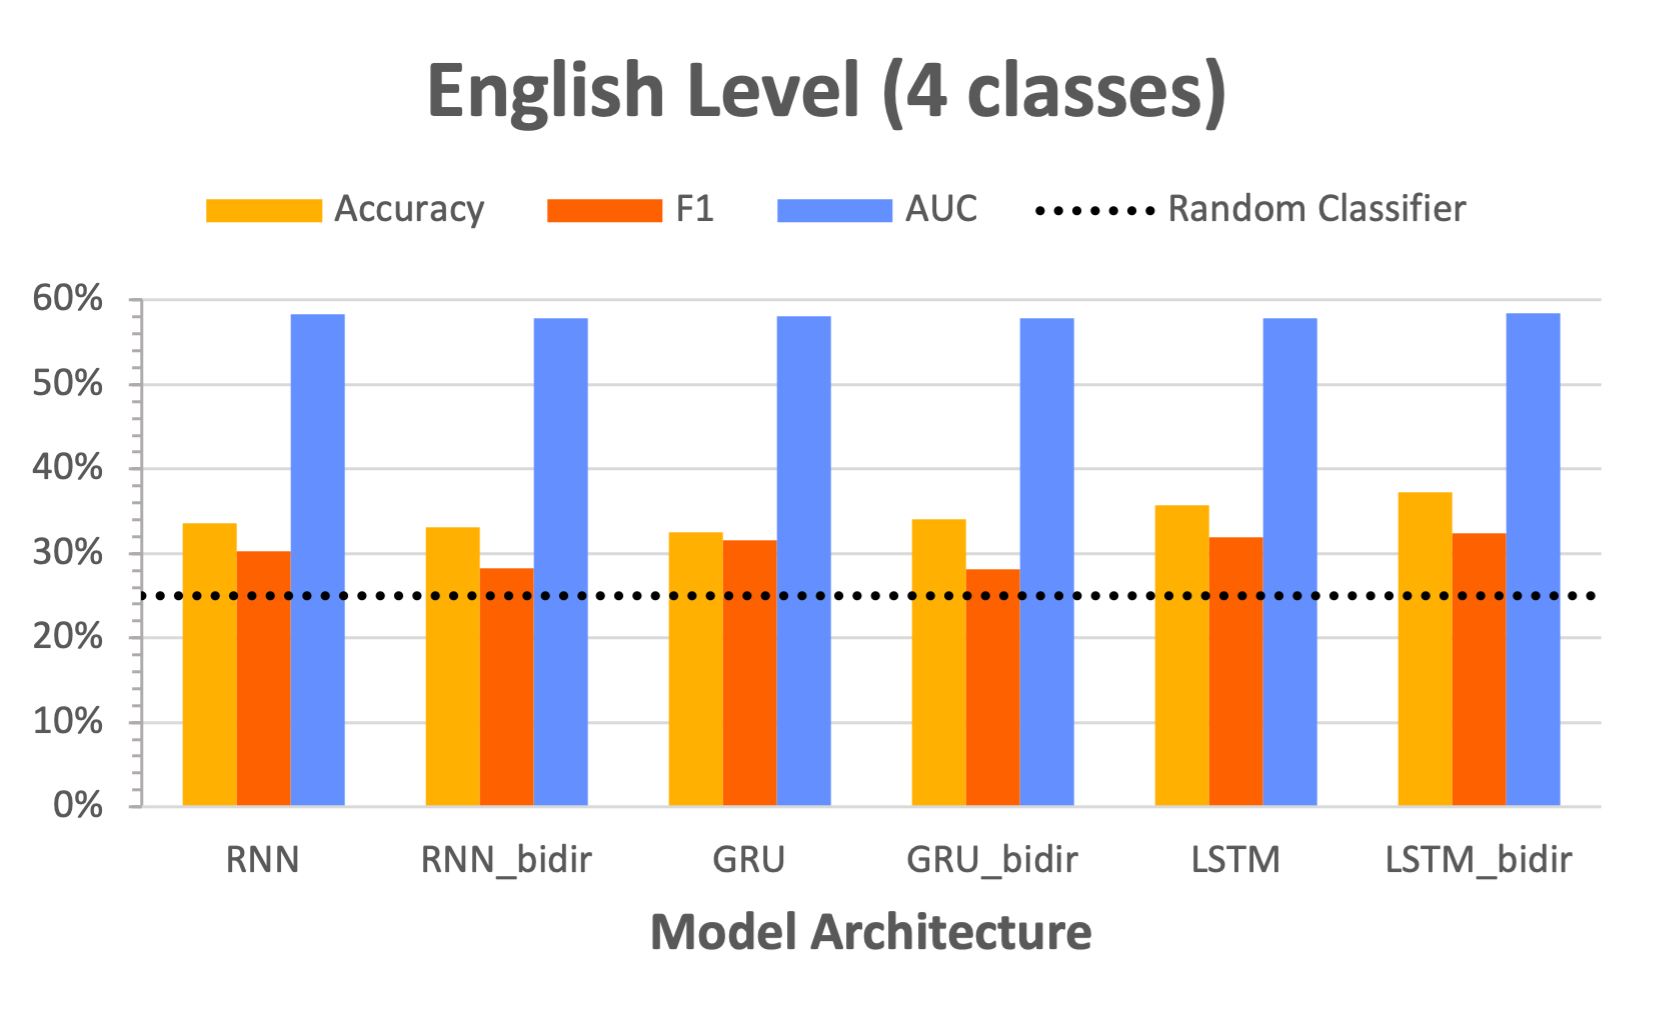
\includegraphics[width=\textwidth]{plots/model_english.png}
         \caption{Layer type}
         \label{fig:models_english}
     \end{subfigure}
     \hfill
     \begin{subfigure}{\w}
         \centering
         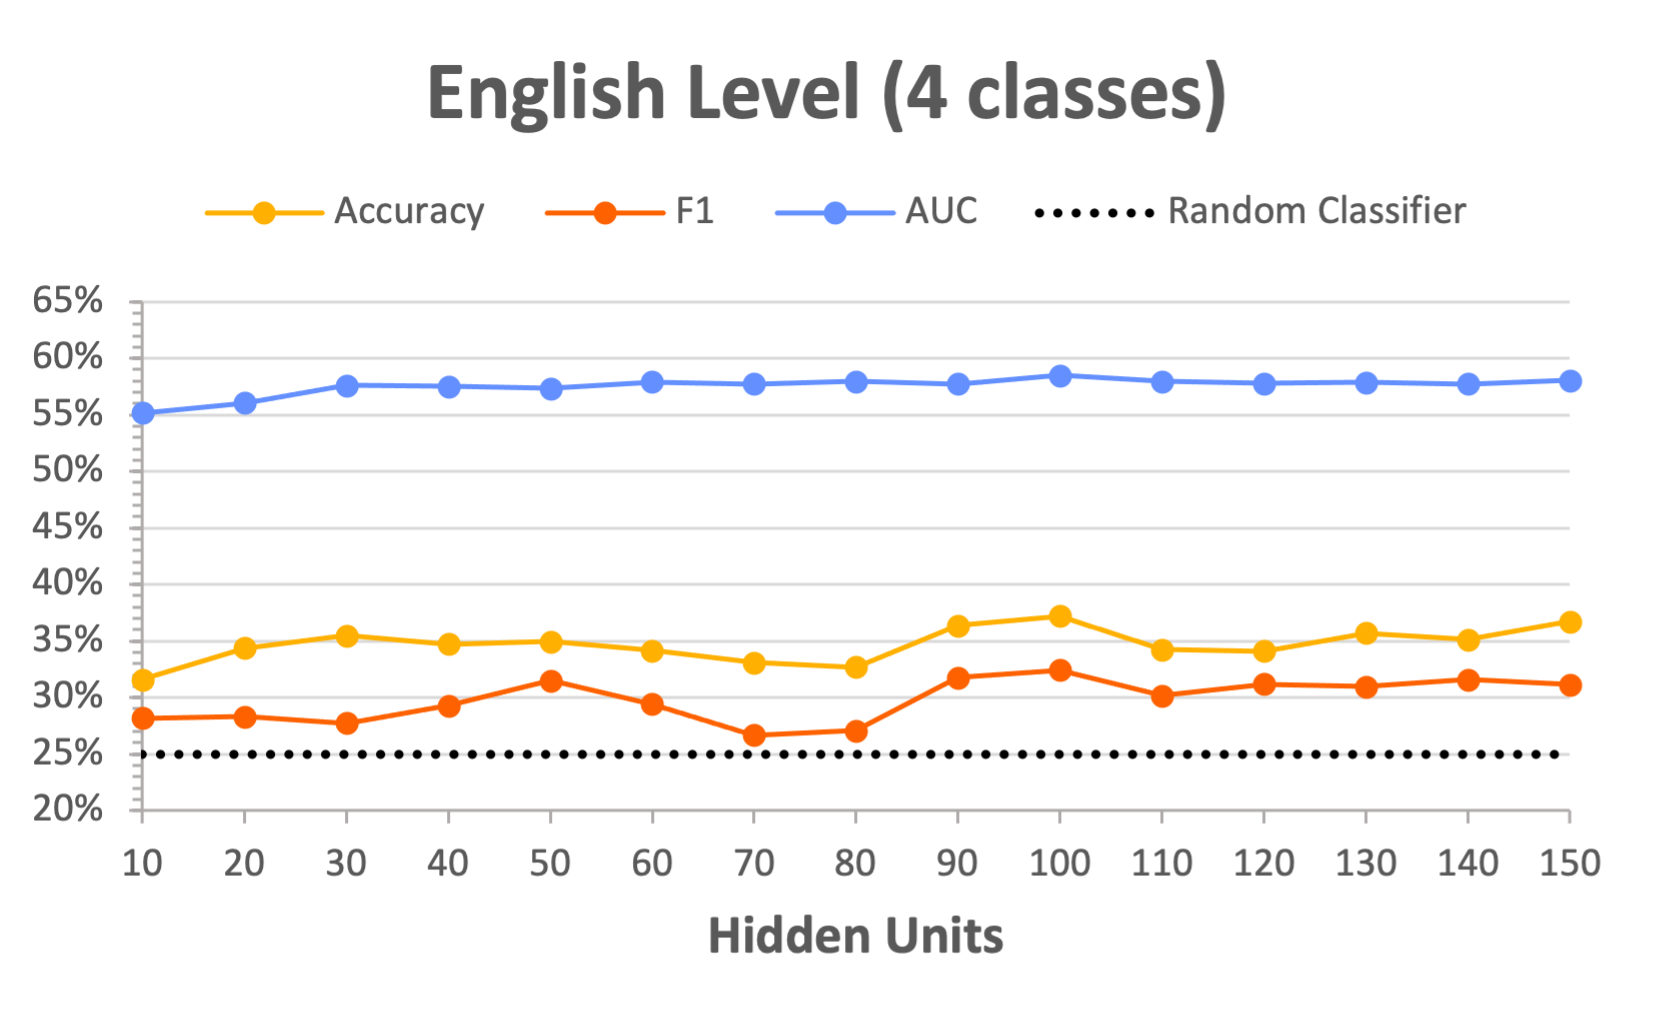
\includegraphics[width=\textwidth]{plots/units_english.png}
         \caption{Hidden Units}
         \label{fig:units_english}
     \end{subfigure}\\
     \begin{subfigure}{\w}
         \centering
         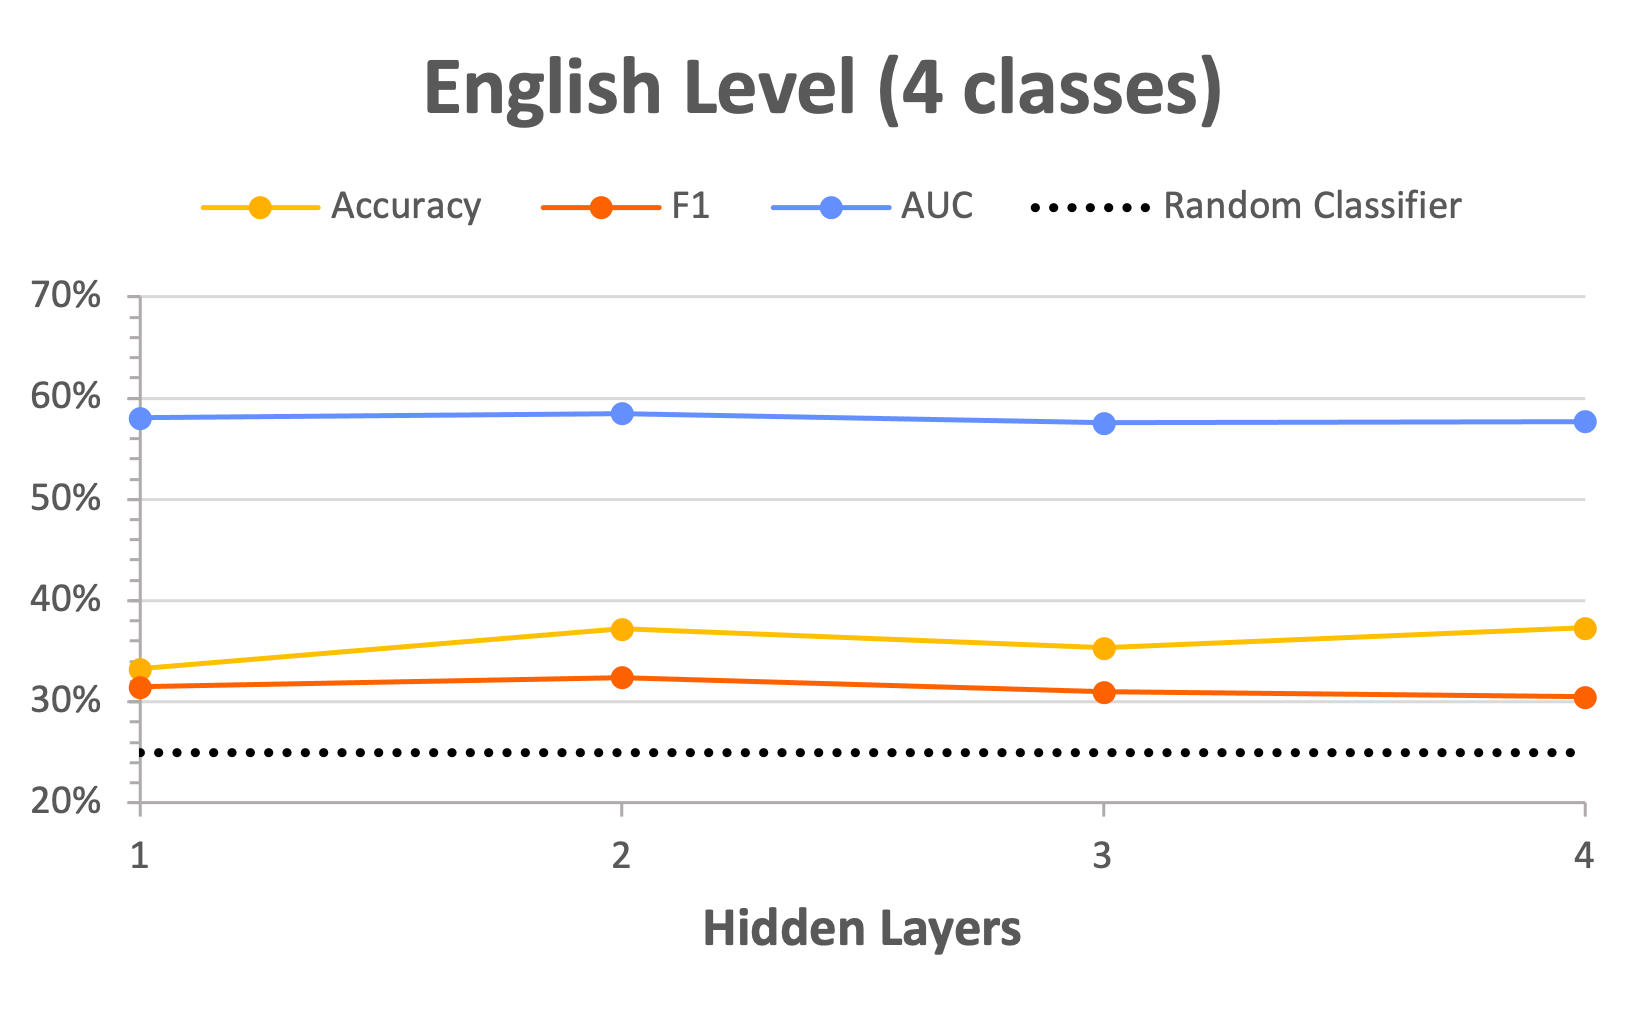
\includegraphics[width=\textwidth]{plots/layers_english.png}
         \caption{Hidden Layers}
         \label{fig:layers_english}
     \end{subfigure}
     \hfill
     \begin{subfigure}{\w}
         \centering
         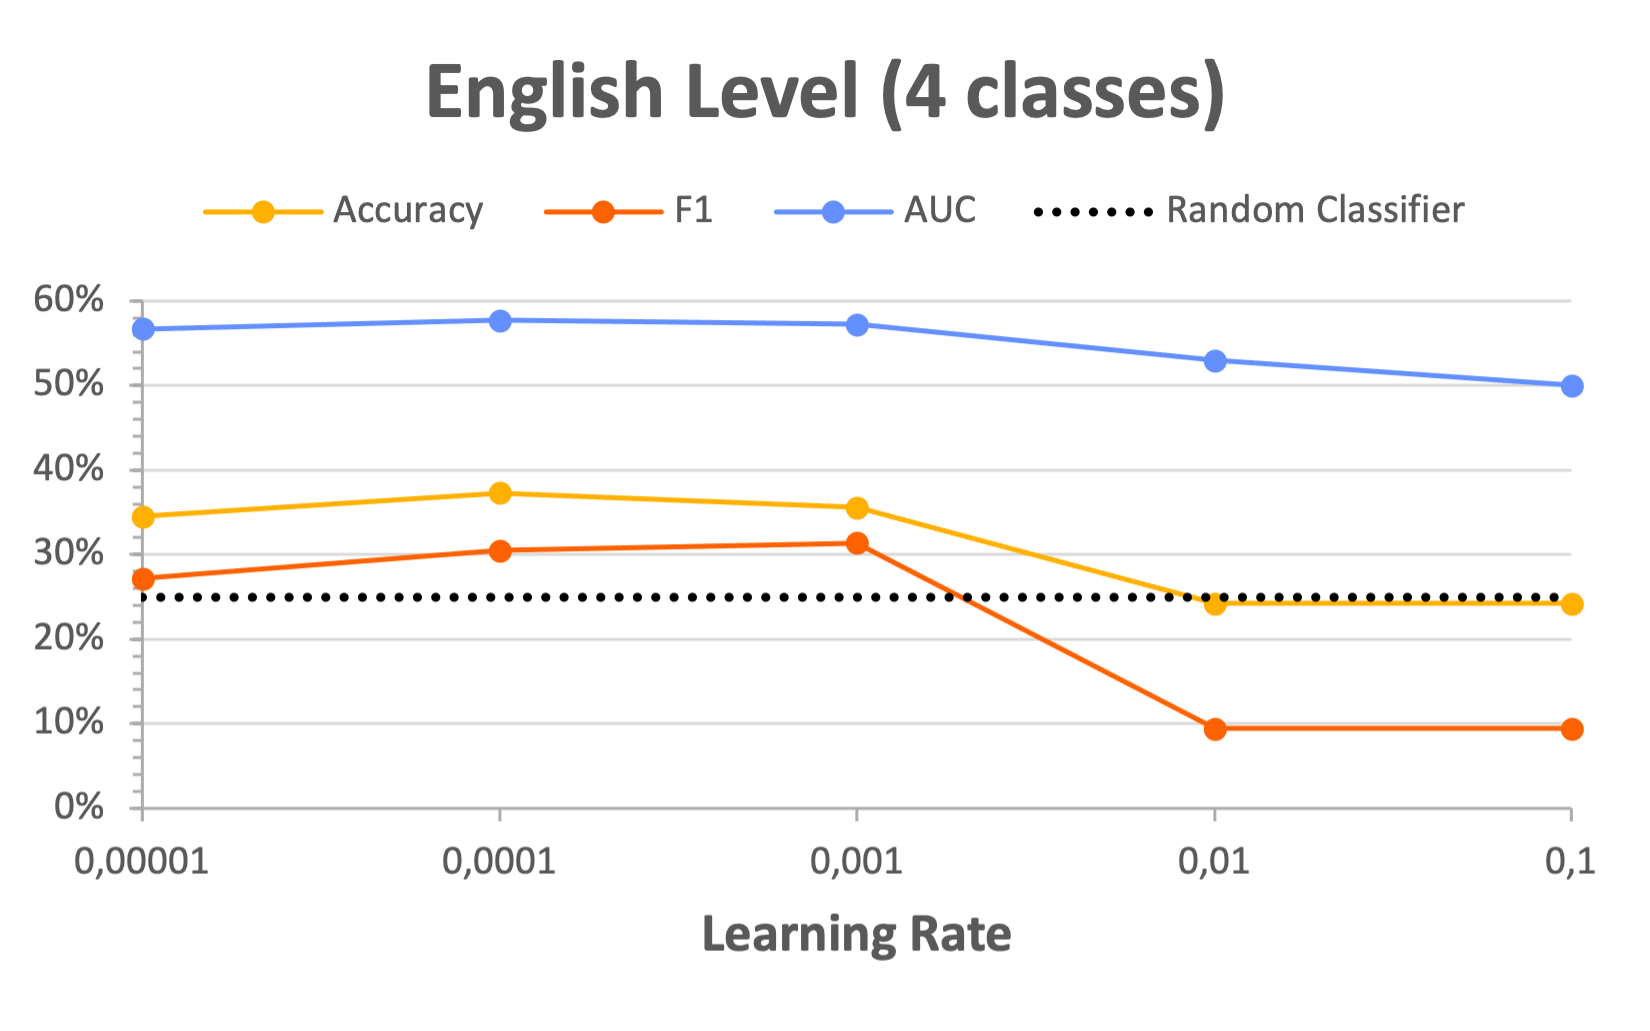
\includegraphics[width=\textwidth]{plots/lr_english.png}
         \caption{Learning Rate}
         \label{fig:lr_english}
     \end{subfigure}

    \caption{Predicting the user's English level from swiped words trajectories.}
    \label{fig:engl}
\end{figure}

\begin{figure}[]
     \centering
     \def\w{0.45\linewidth}
     \begin{subfigure}{\w}
         \centering
         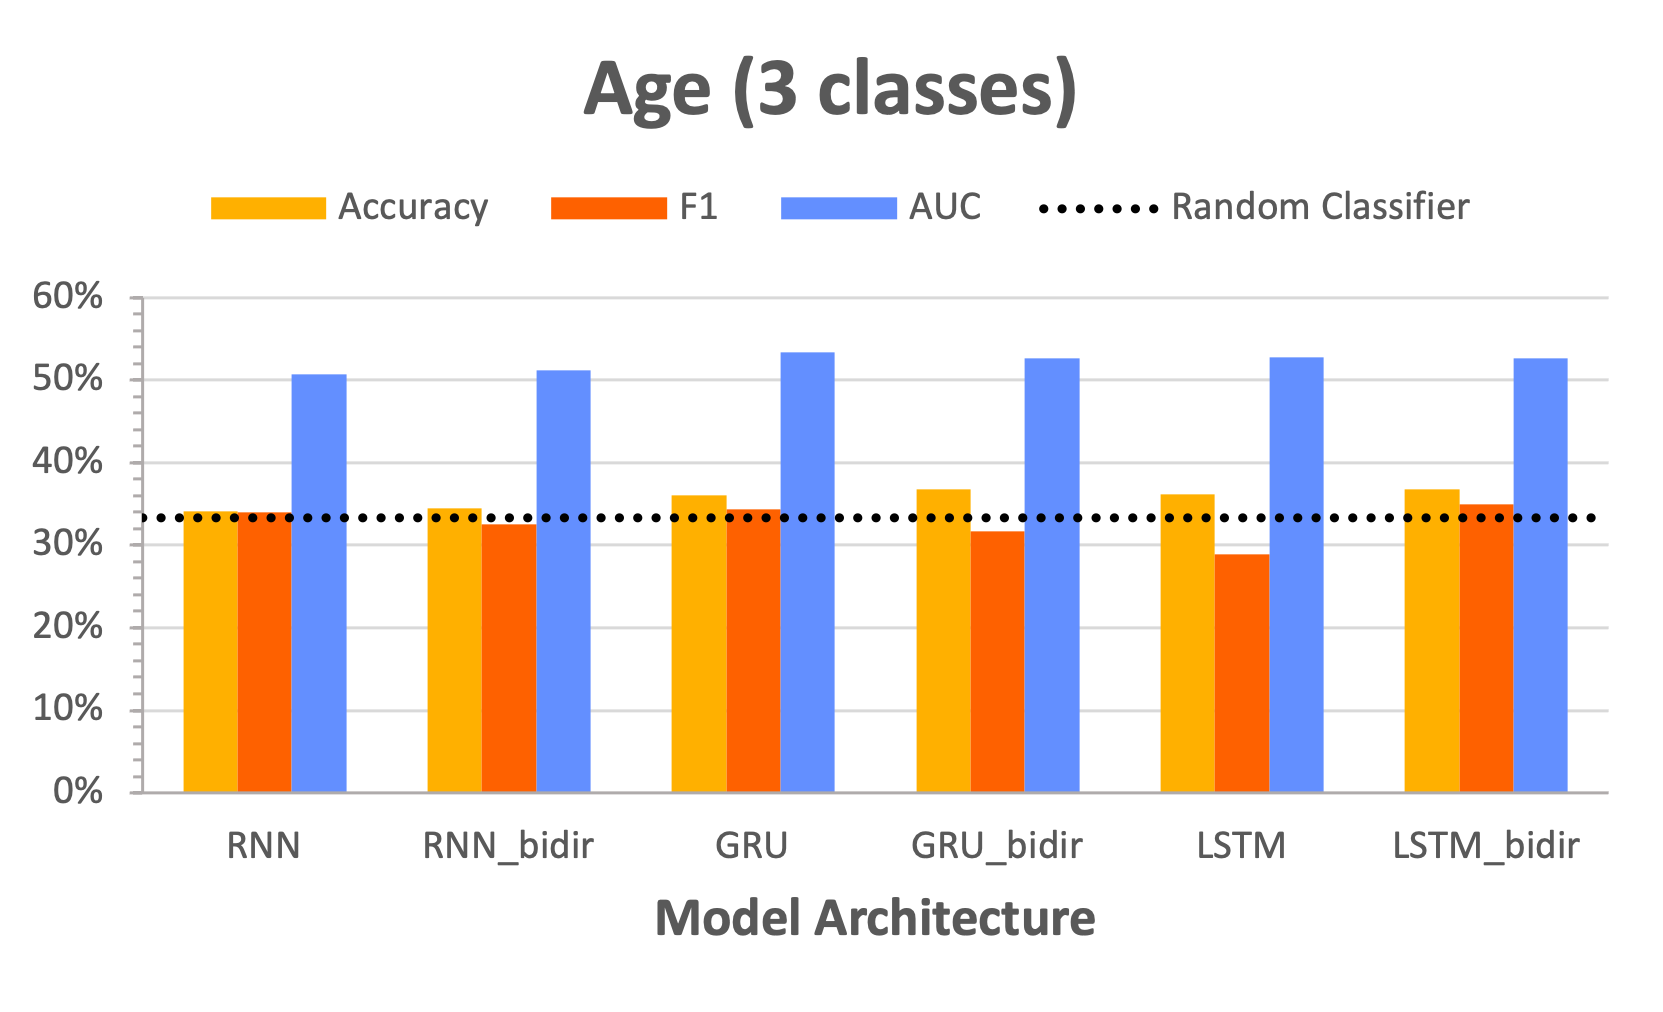
\includegraphics[width=\textwidth]{plots/model_age.png}
         \caption{Layer type}
         \label{fig:models_age}
     \end{subfigure}
     \hfill
     \begin{subfigure}{\w}
         \centering
         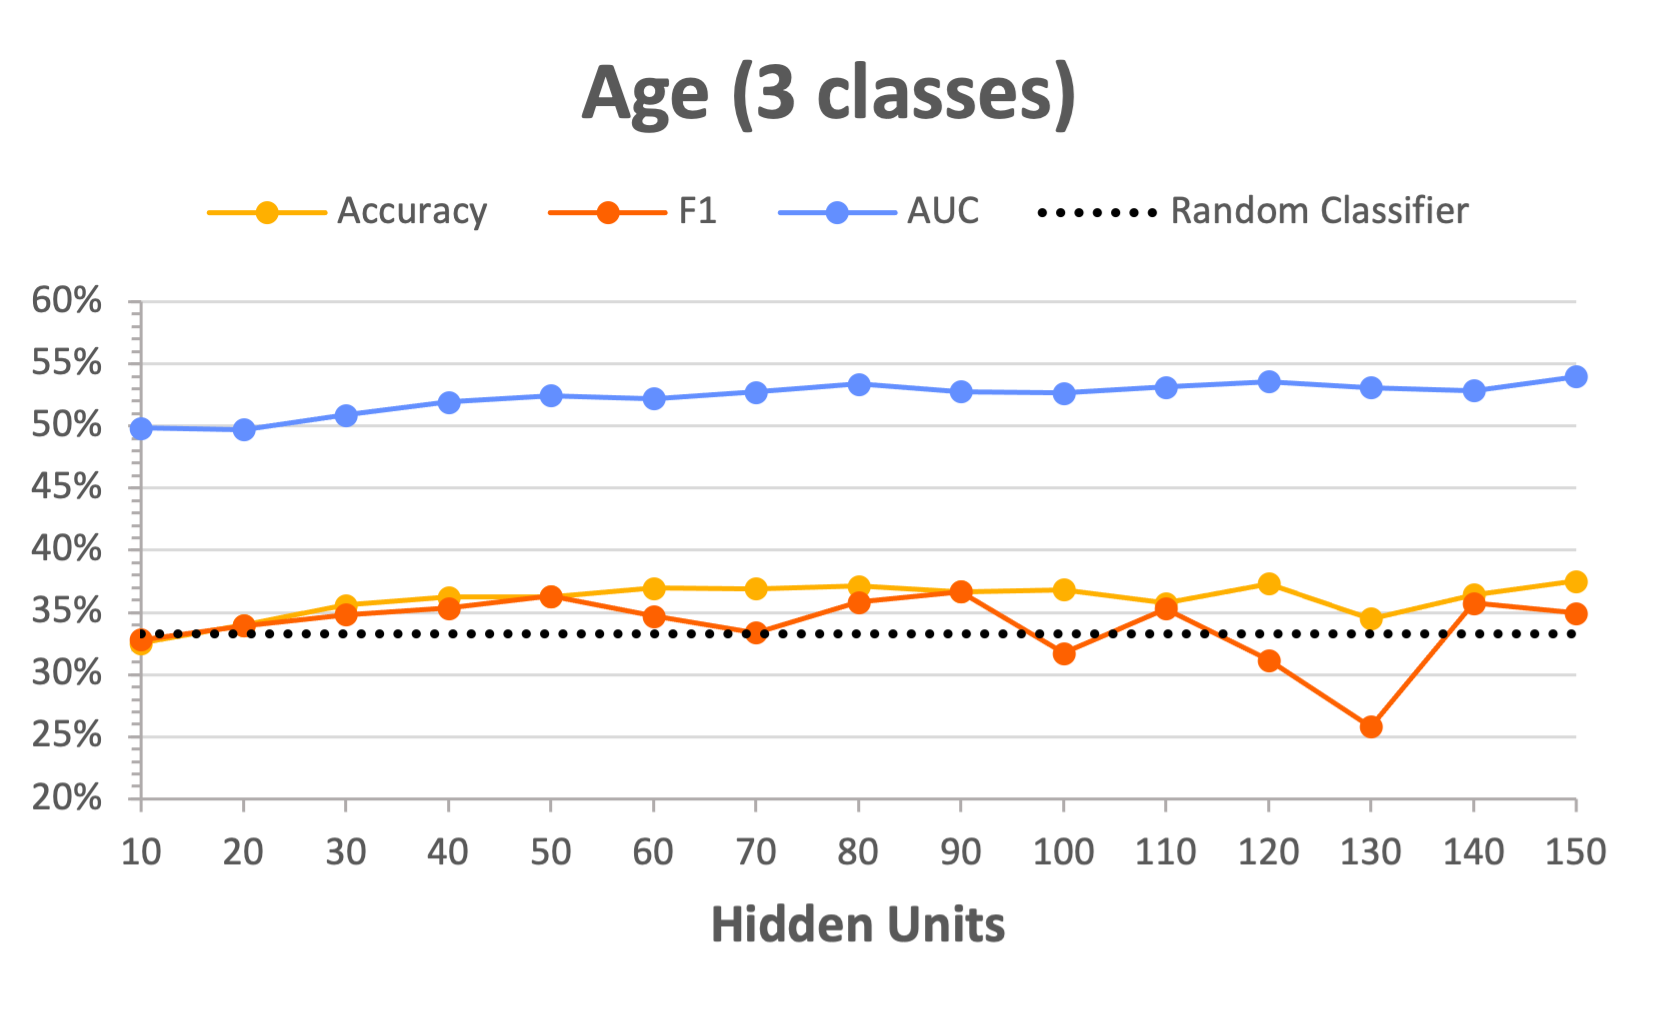
\includegraphics[width=\textwidth]{plots/units_age.png}
         \caption{Hidden Units}
         \label{fig:units_age}
     \end{subfigure}\\
     \begin{subfigure}{\w}
         \centering
         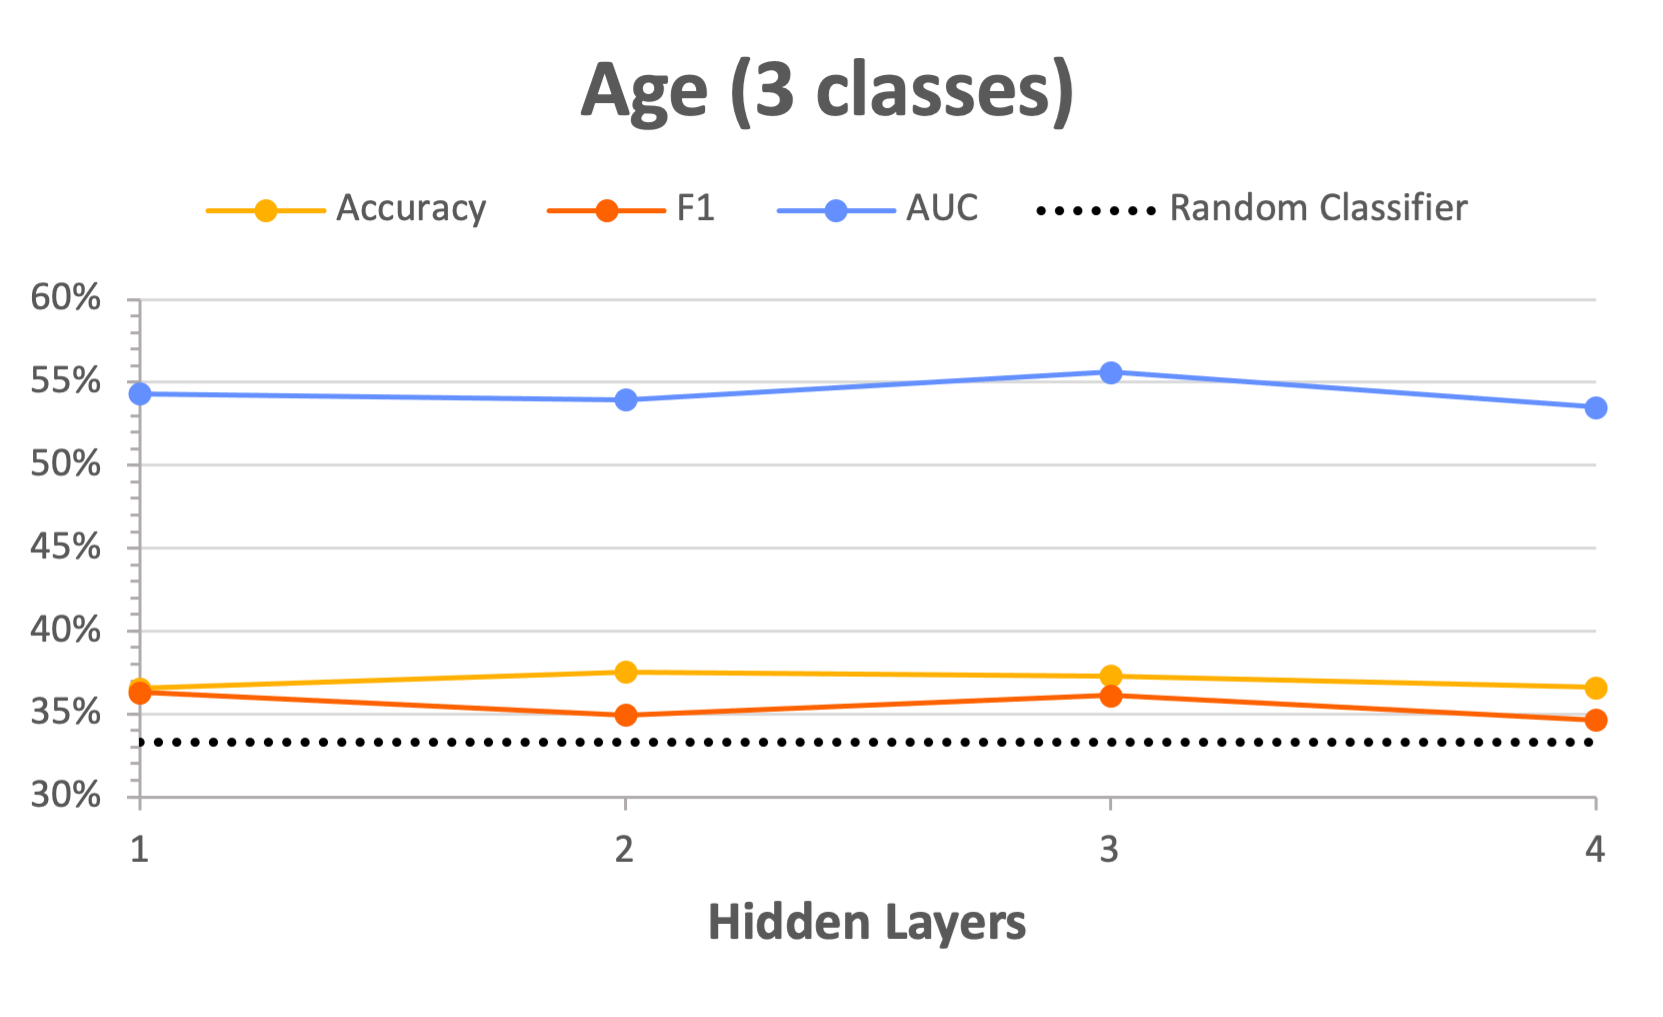
\includegraphics[width=\textwidth]{plots/layers_age.png}
         \caption{Hidden Layers}
         \label{fig:layers_age}
     \end{subfigure}
     \hfill
     \begin{subfigure}{\w}
         \centering
         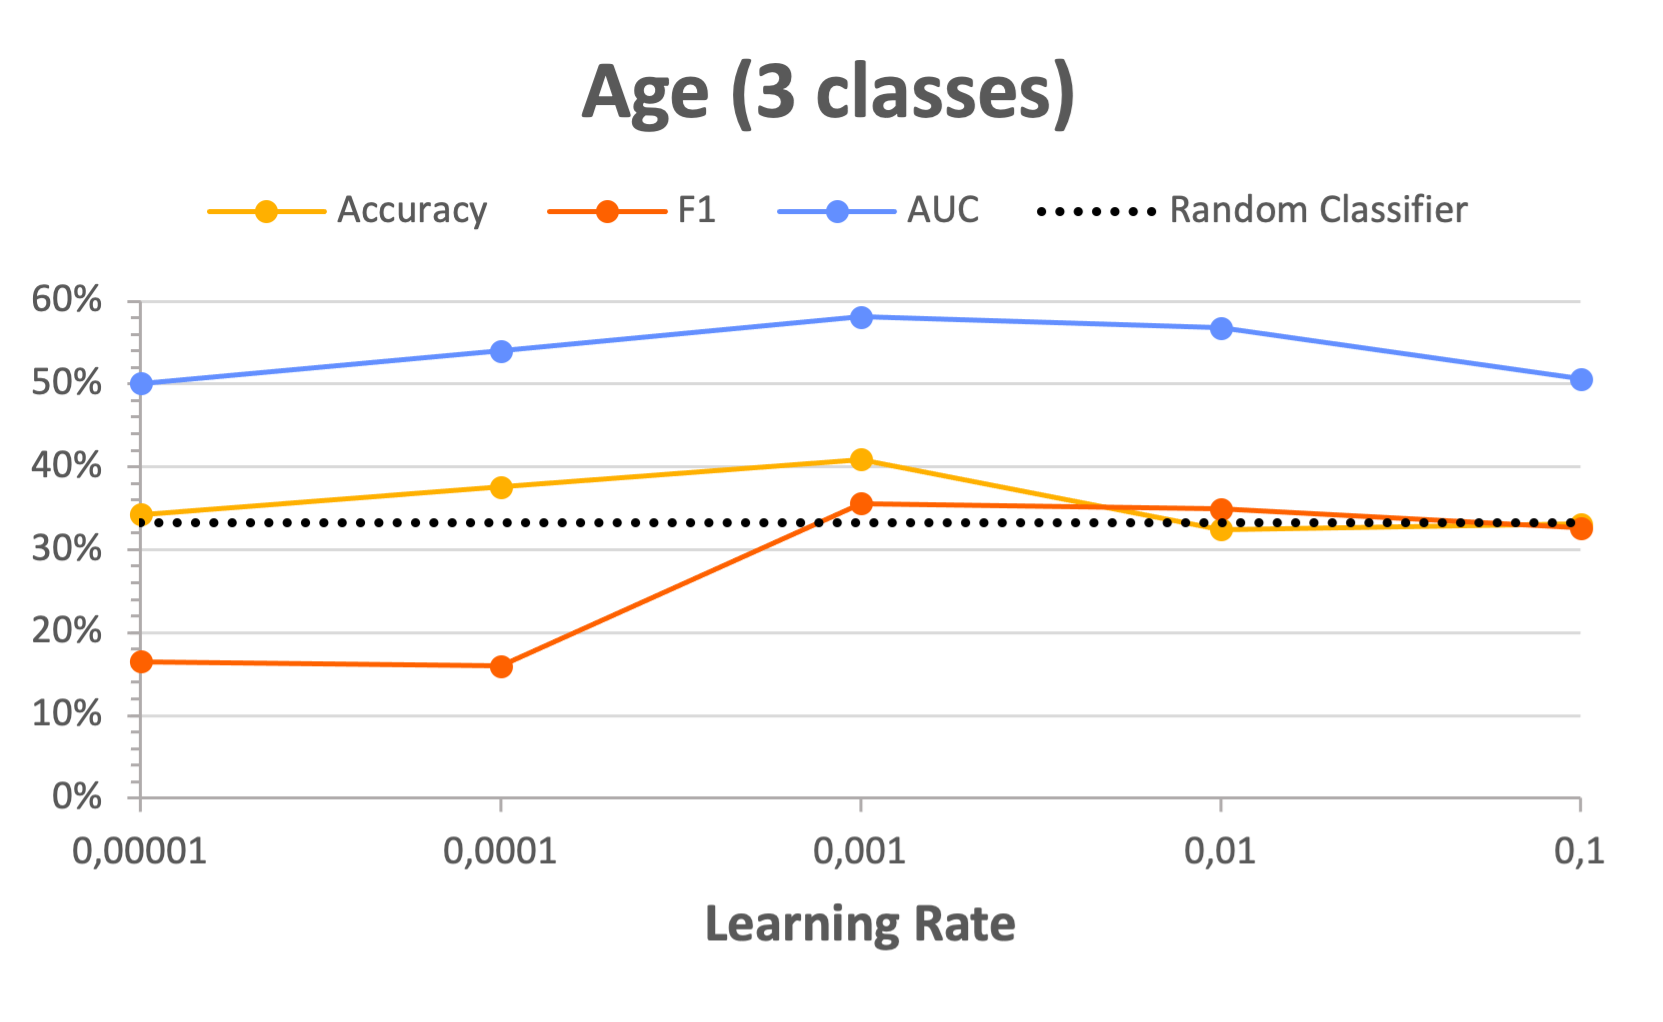
\includegraphics[width=\textwidth]{plots/lr_age.png}
         \caption{Learning Rate}
         \label{fig:lr_age}
     \end{subfigure}

    \caption{Predicting the user's age from swiped words trajectories.}
    \label{fig:age}
\end{figure}

\begin{figure}[]
     \centering
     \def\w{0.4\linewidth}
     \begin{subfigure}{\w}
         \centering
         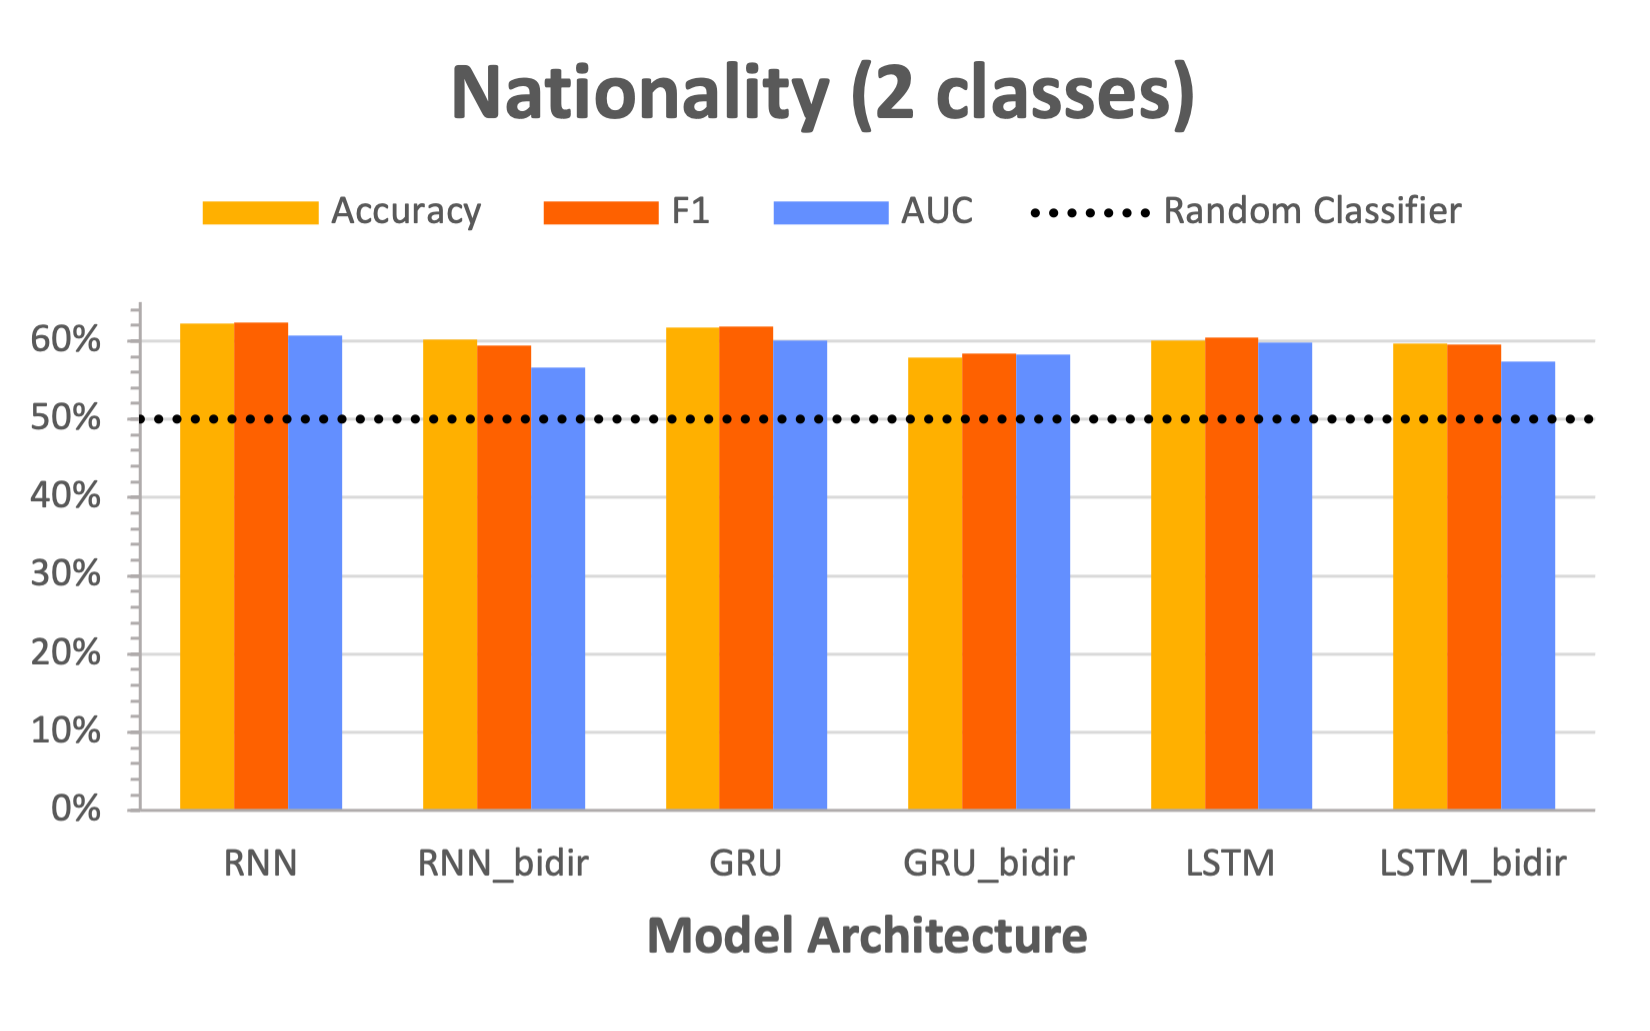
\includegraphics[width=\textwidth]{plots/model_nat.png}
         \caption{Layer type}
         \label{fig:models_nat}
     \end{subfigure}
     \hfill
     \begin{subfigure}{\w}
         \centering
         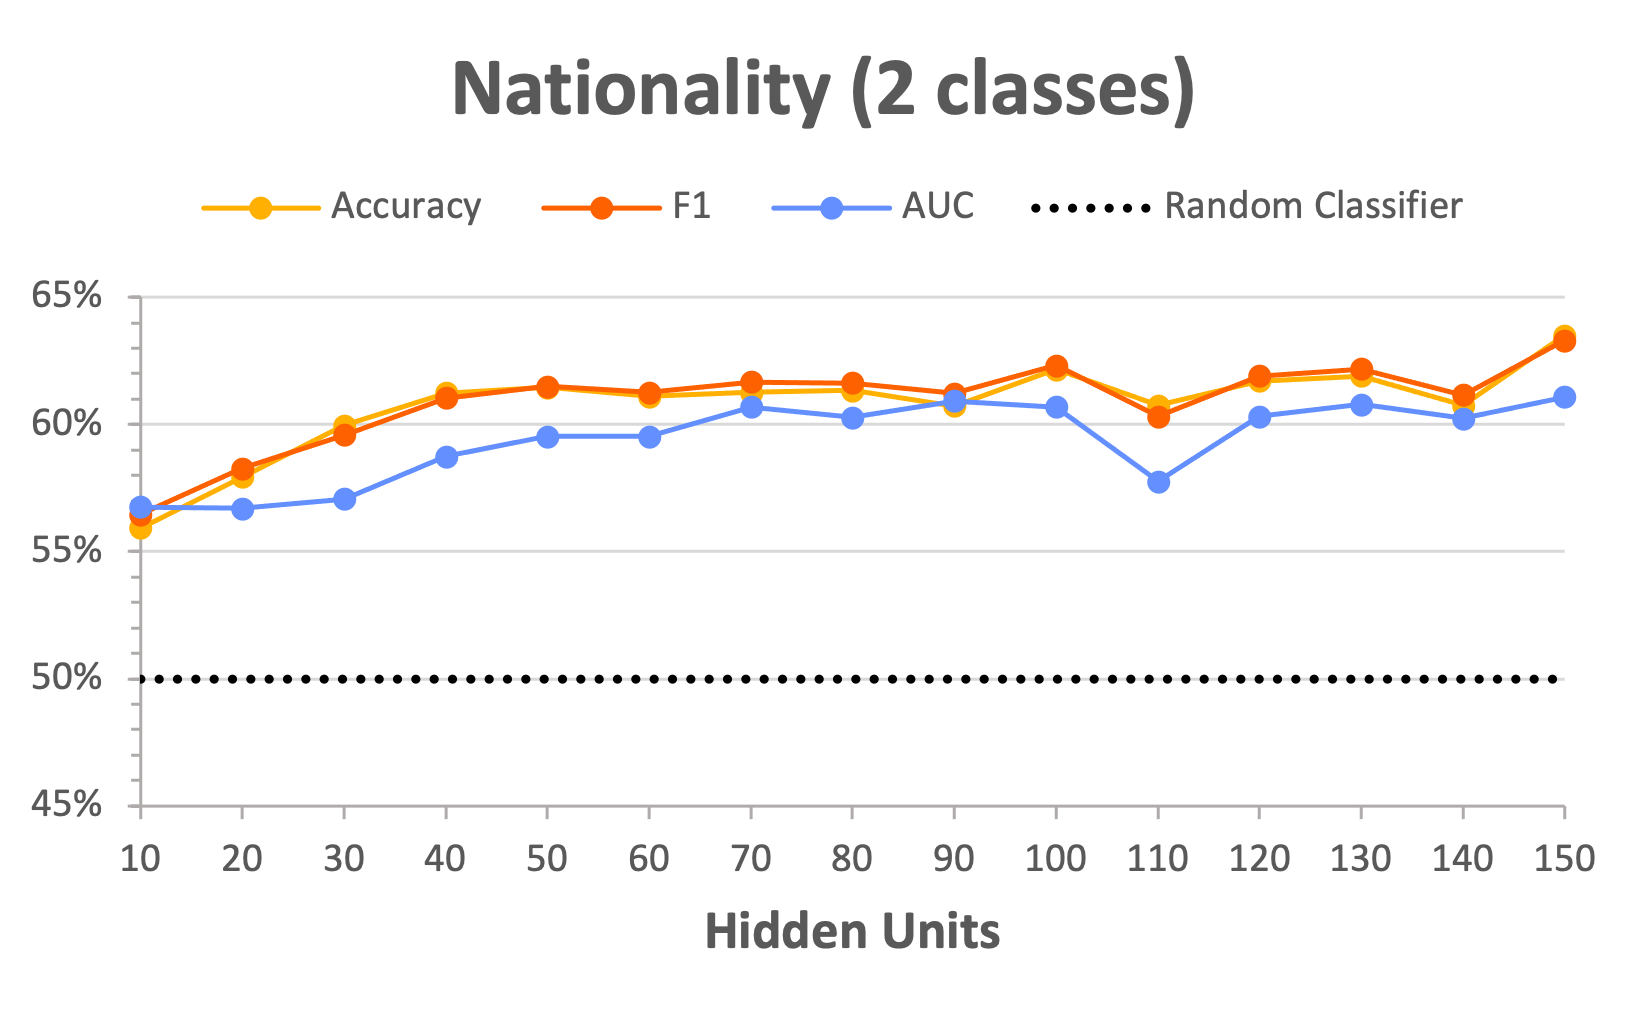
\includegraphics[width=\textwidth]{plots/units_nat.png}
         \caption{Hidden Units}
         \label{fig:units_nat}
     \end{subfigure}\\
     \begin{subfigure}{\w}
         \centering
         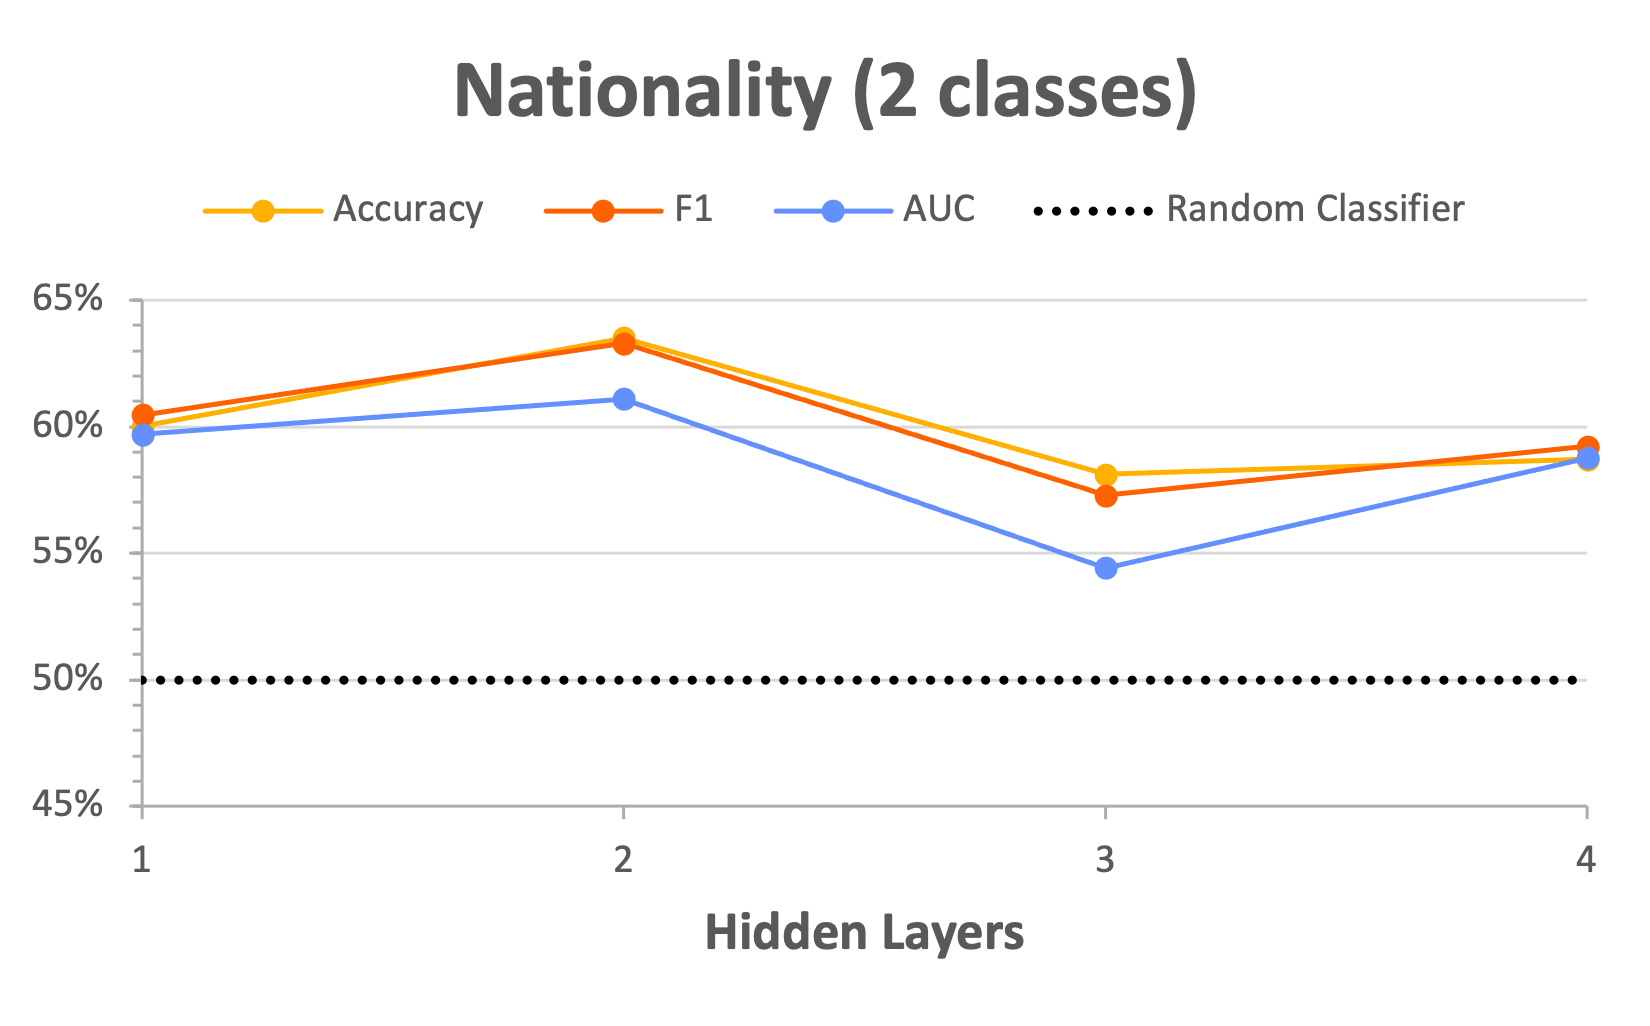
\includegraphics[width=\textwidth]{plots/layers_nat.png}
         \caption{Hidden Layers}
         \label{fig:layers_nat}
     \end{subfigure}
     \hfill
     \begin{subfigure}{\w}
         \centering
         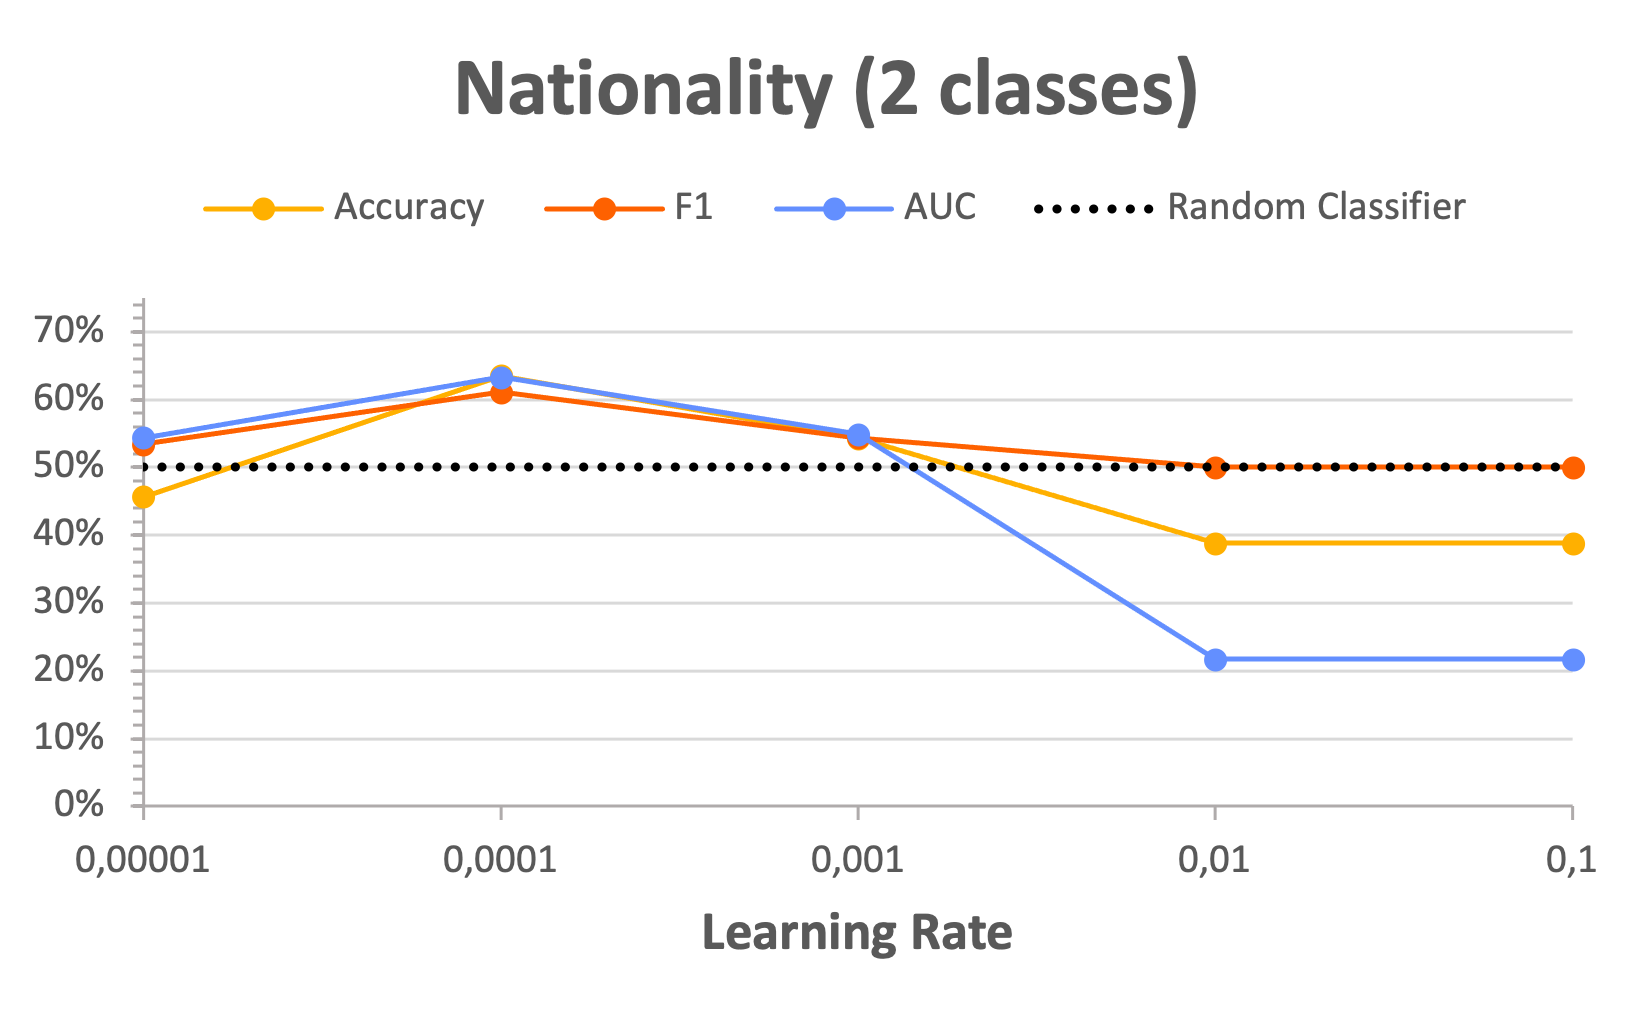
\includegraphics[width=\textwidth]{plots/lr_nat.png}
         \caption{Learning Rate}
         \label{fig:lr_nat}
     \end{subfigure}

    \caption{Predicting the user's nationality from swiped words trajectories.}
    \label{fig:nat}
\end{figure}

\begin{figure}[]
     \centering
     \def\w{0.45\linewidth}
     \begin{subfigure}{\w}
         \centering
         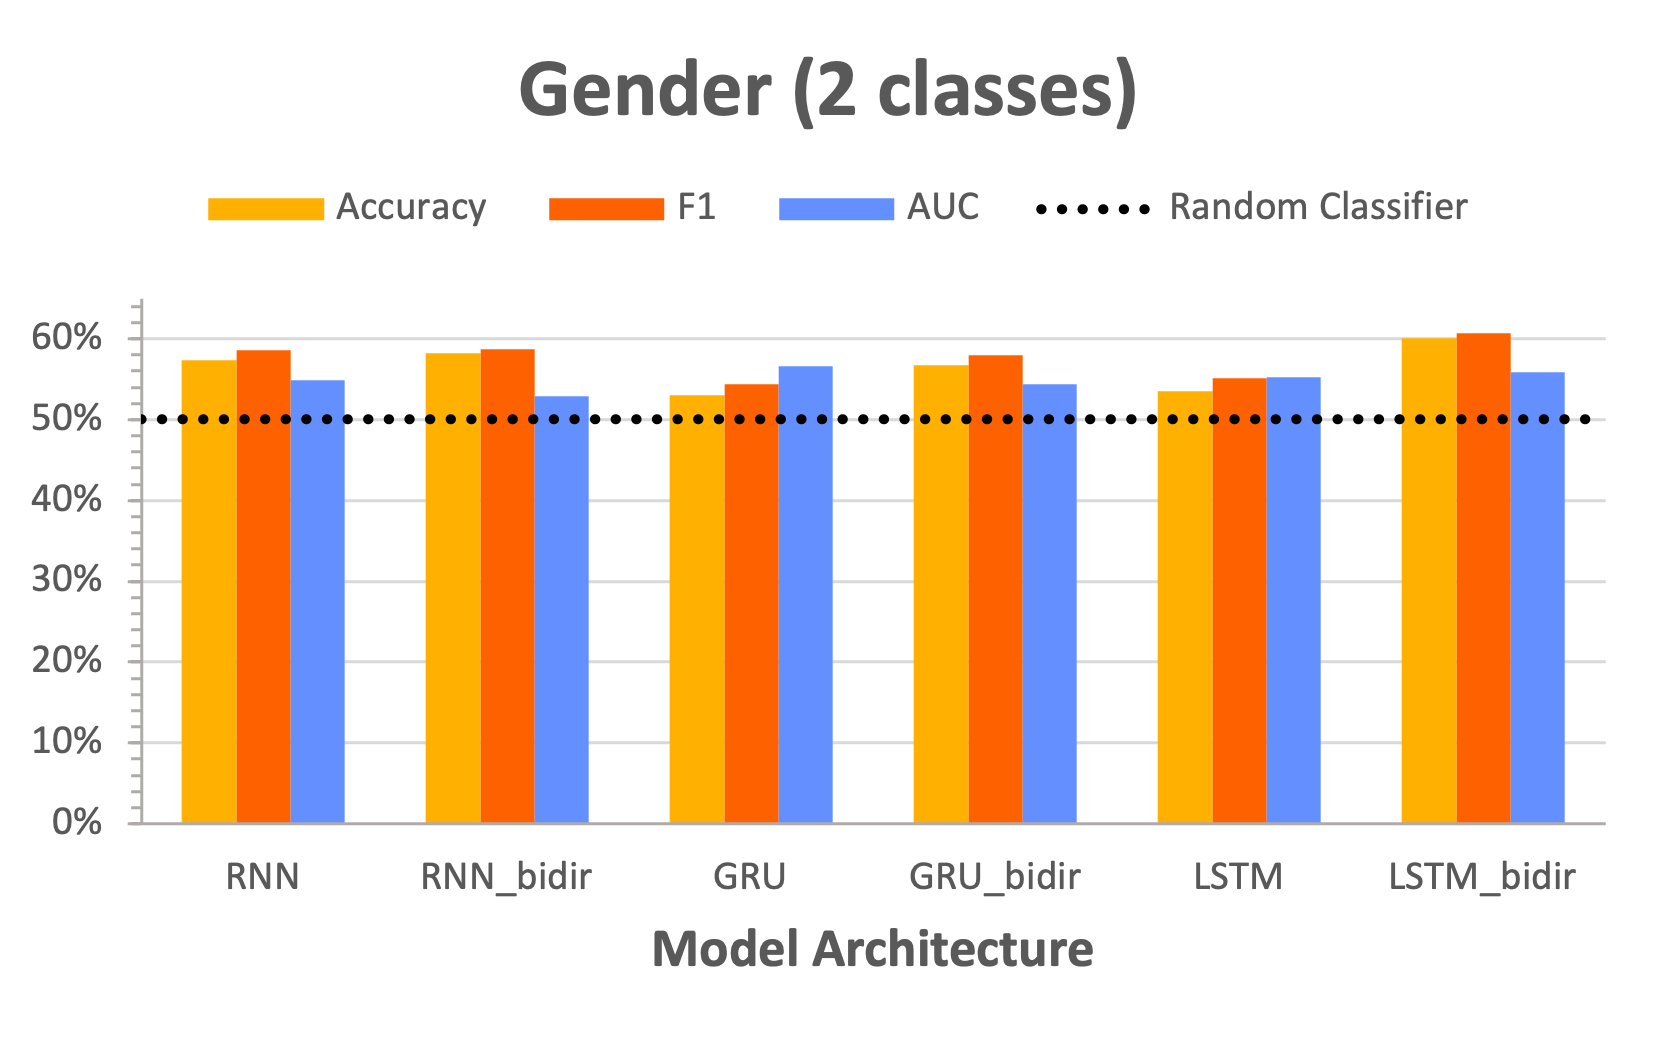
\includegraphics[width=\textwidth]{plots/model_gender.png}
         \caption{Layer type}
         \label{fig:models_gender}
     \end{subfigure}
     \hfill
     \begin{subfigure}{\w}
         \centering
         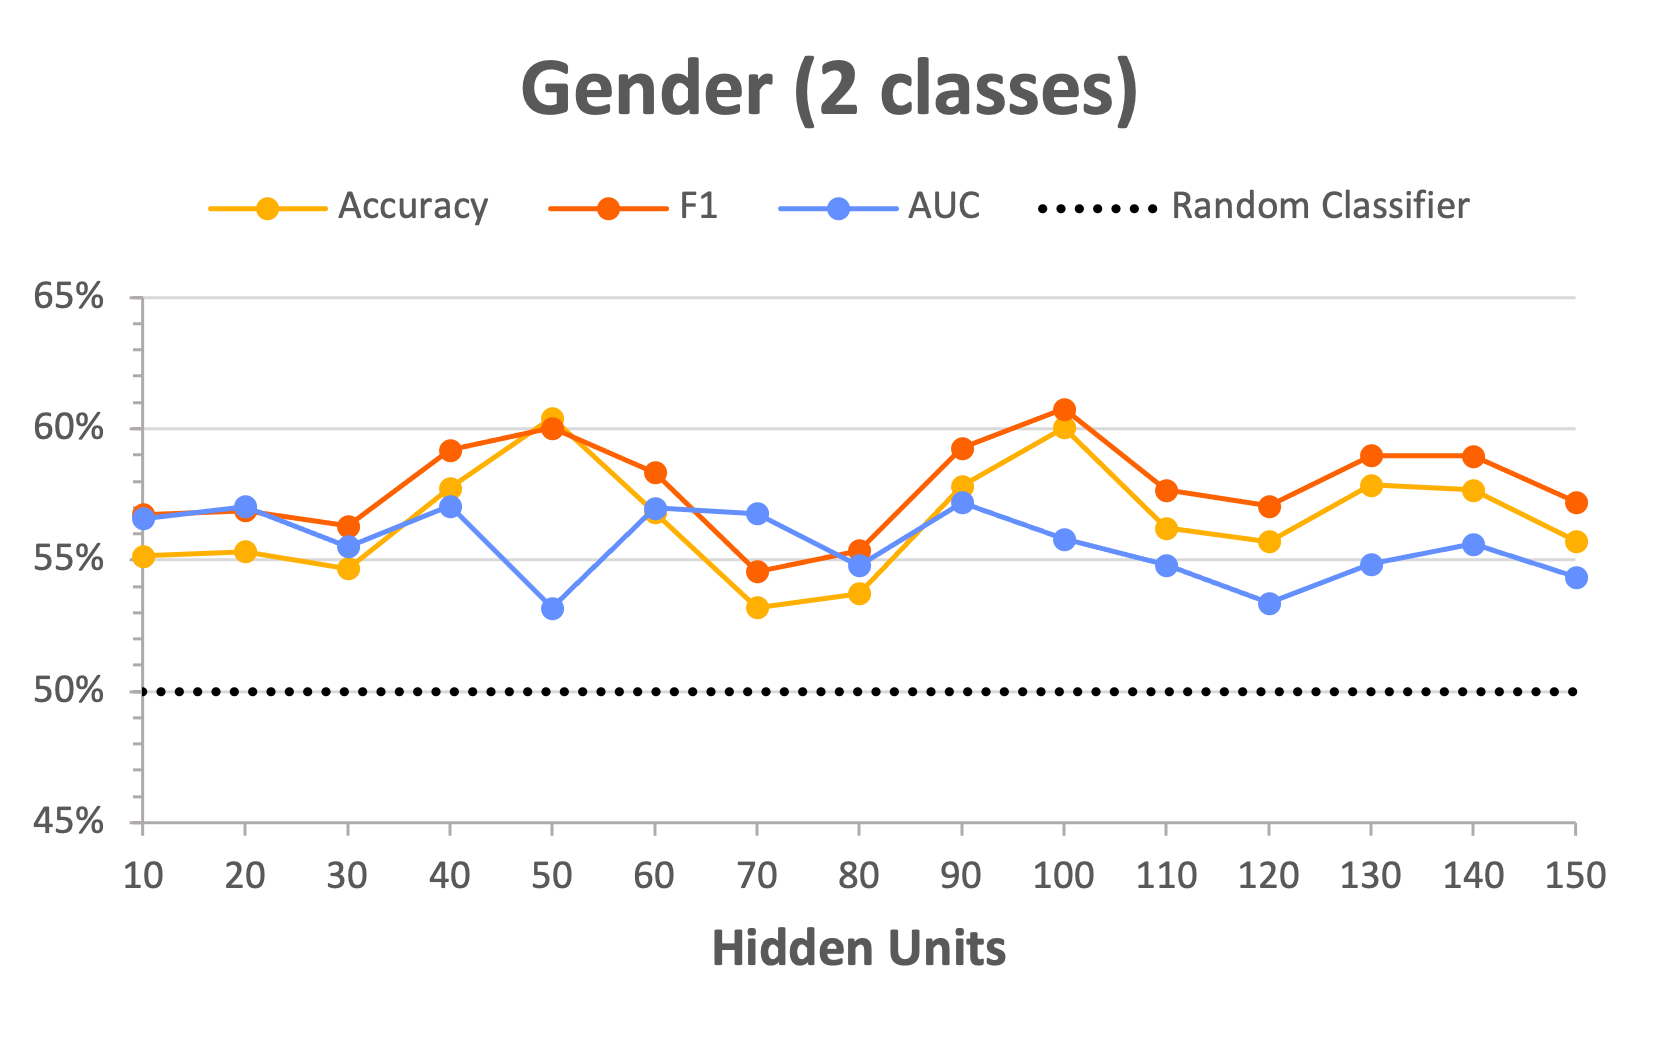
\includegraphics[width=\textwidth]{plots/units_gender.png}
         \caption{Hidden Units}
         \label{fig:units_gender}
     \end{subfigure}\\
     \begin{subfigure}{\w}
         \centering
         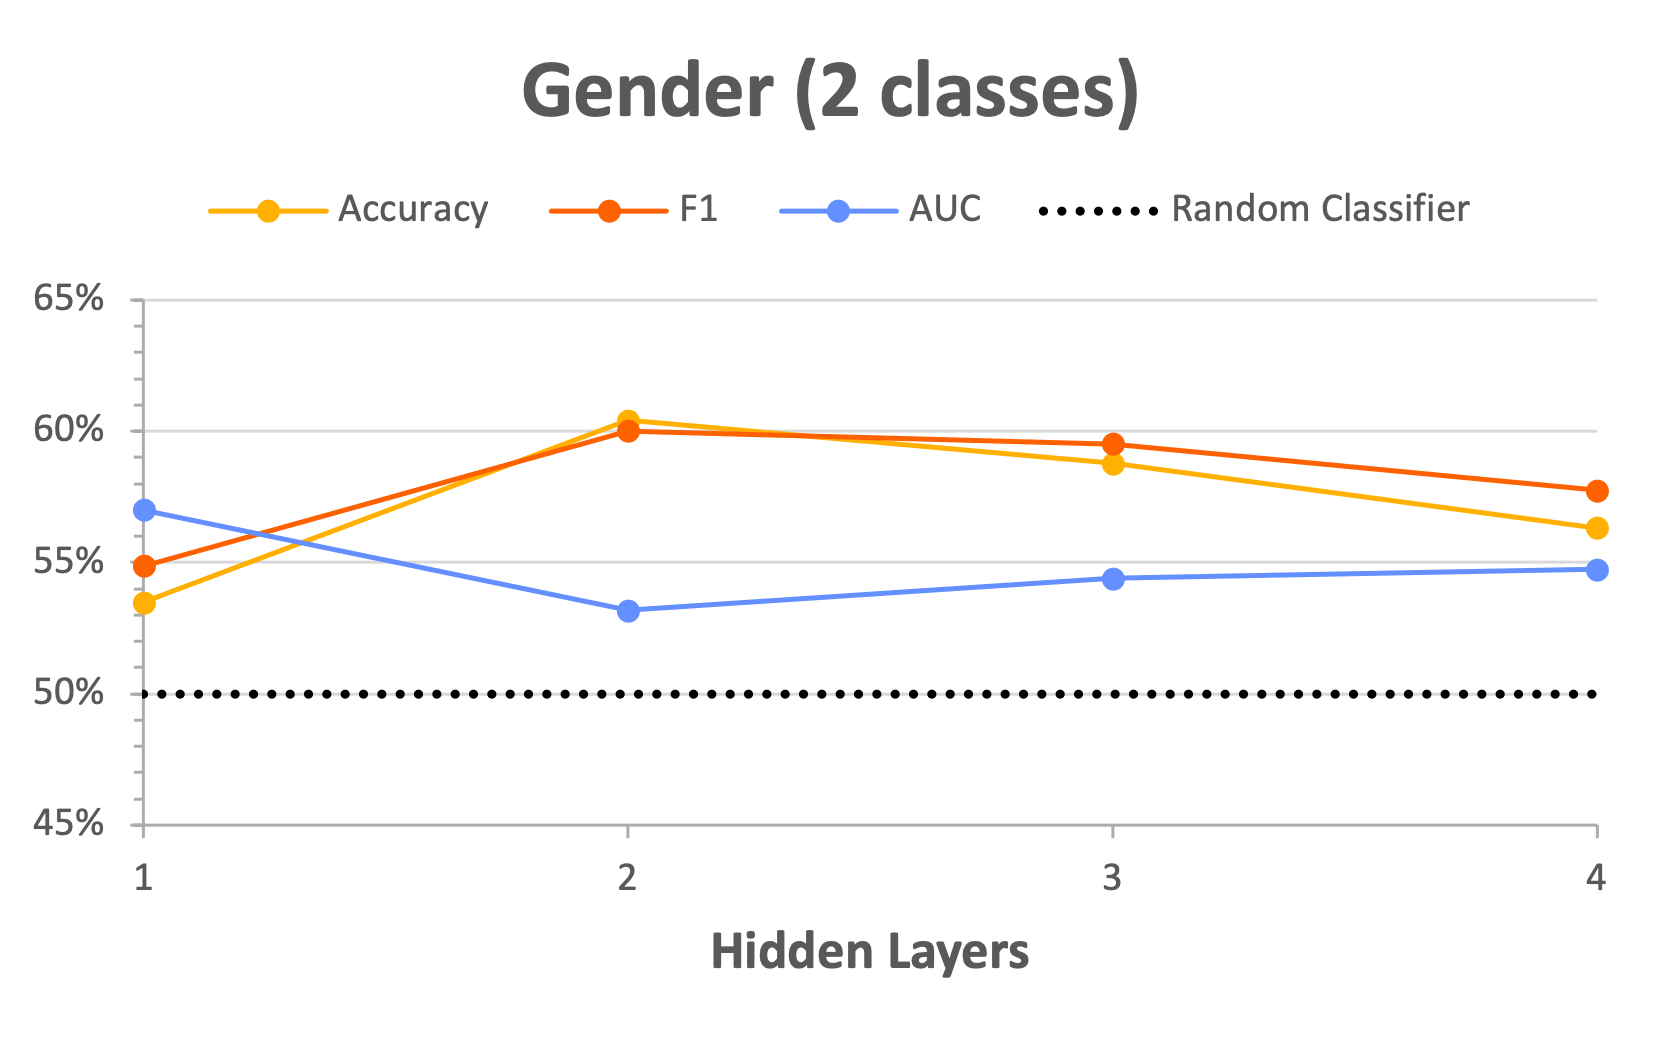
\includegraphics[width=\textwidth]{plots/layers_gender.png}
         \caption{Hidden Layers}
         \label{fig:layers_gender}
     \end{subfigure}
     \hfill
     \begin{subfigure}{\w}
         \centering
         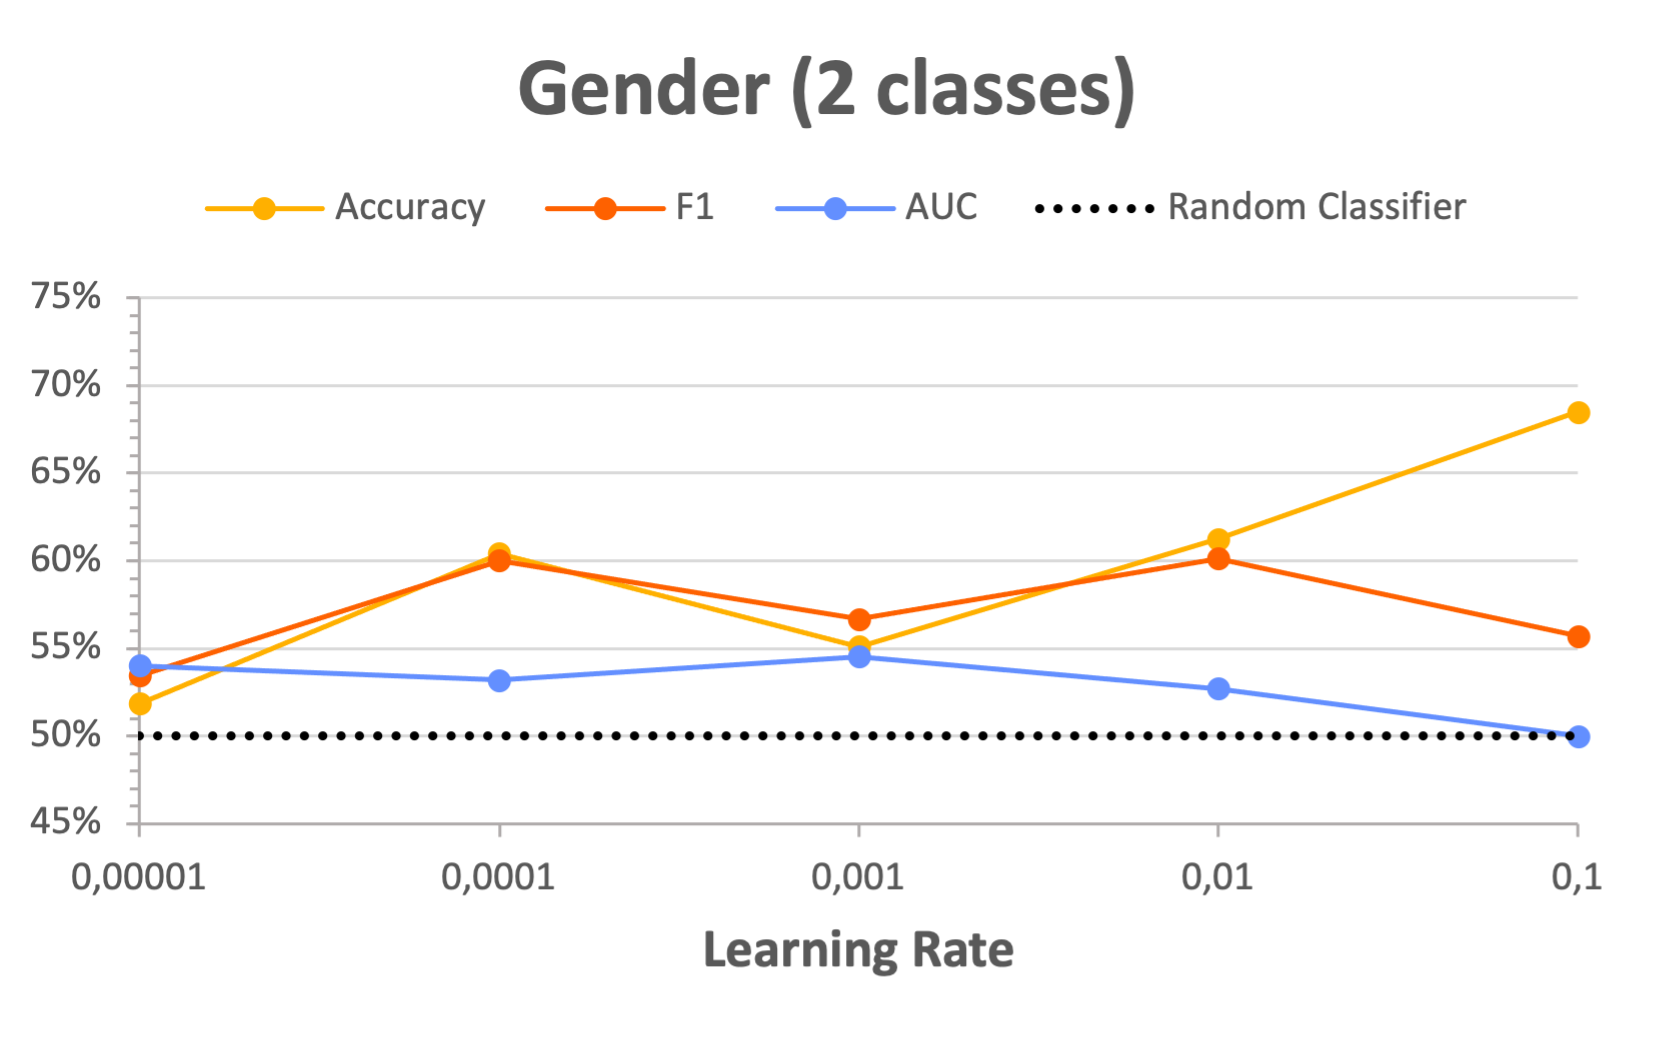
\includegraphics[width=\textwidth]{plots/lr_gender.png}
         \caption{Learning Rate}
         \label{fig:lr_gender}
     \end{subfigure}

    \caption{Predicting the user's gender from swiped words trajectories.}
    \label{fig:gender}
\end{figure}

\begin{figure}[]
     \centering
     \def\w{0.45\linewidth}
     \begin{subfigure}{\w}
         \centering
         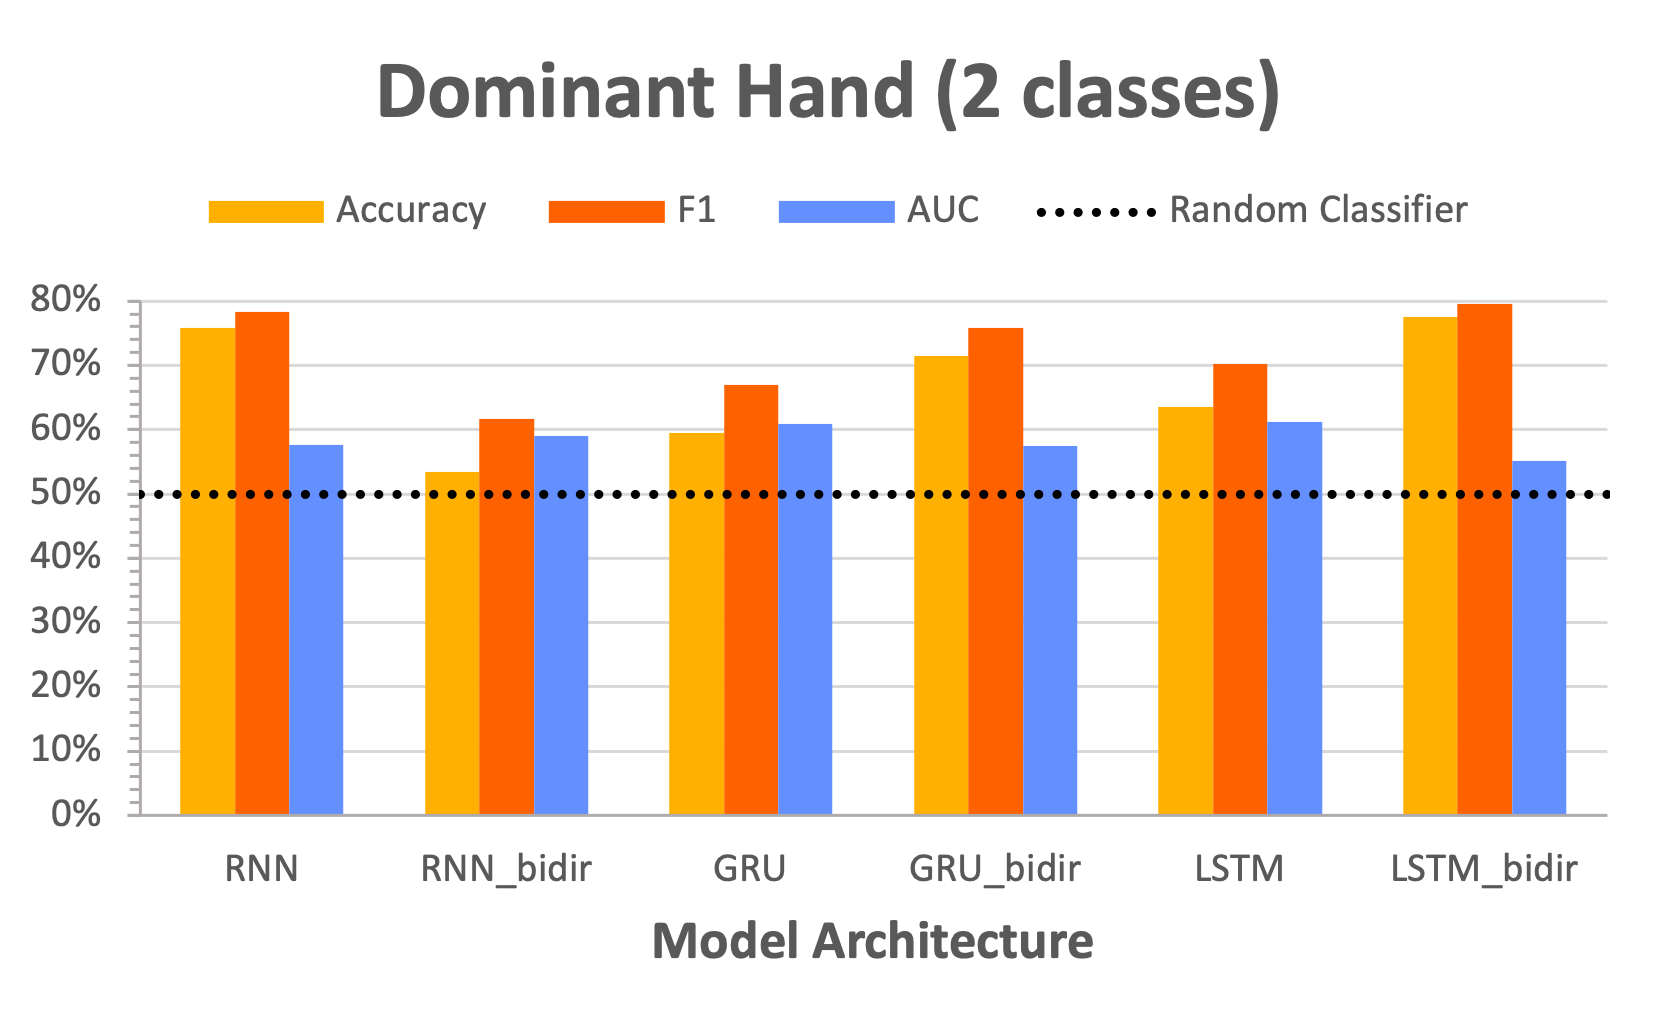
\includegraphics[width=\textwidth]{plots/model_dom.png}
         \caption{Layer type}
         \label{fig:models_dom}
     \end{subfigure}
     \hfill
     \begin{subfigure}{\w}
         \centering
         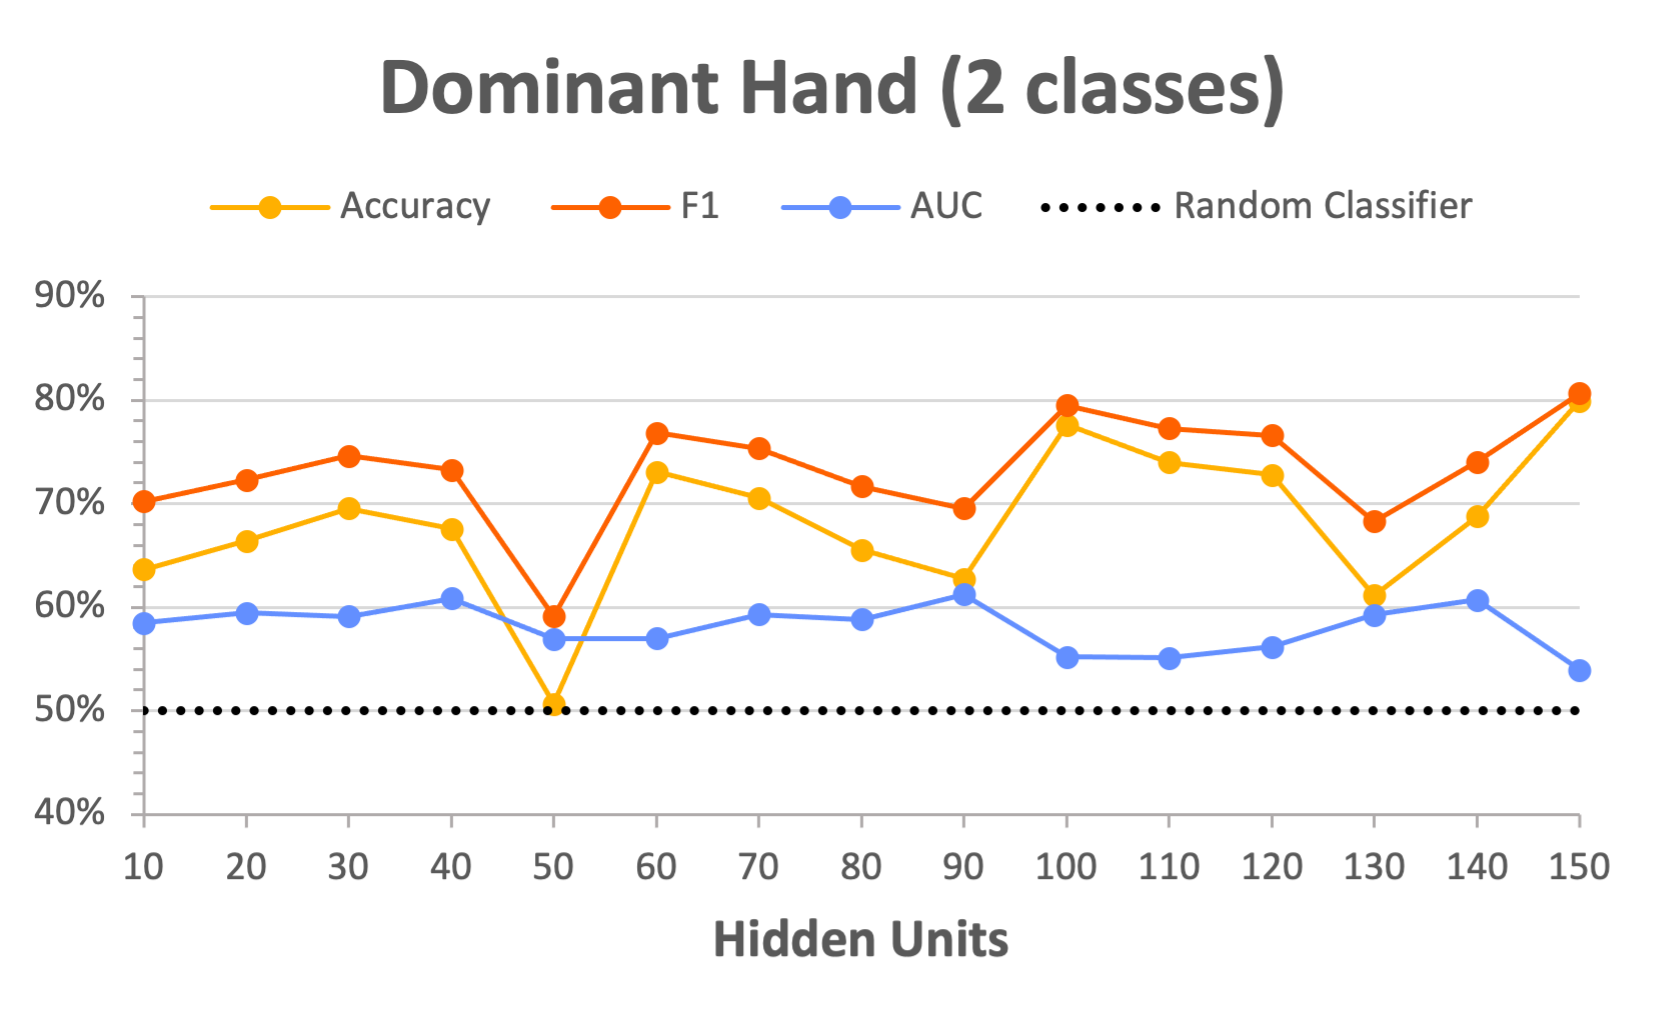
\includegraphics[width=\textwidth]{plots/units_dom.png}
         \caption{Hidden Units}
         \label{fig:units_dom}
     \end{subfigure}\\
     \begin{subfigure}{\w}
         \centering
         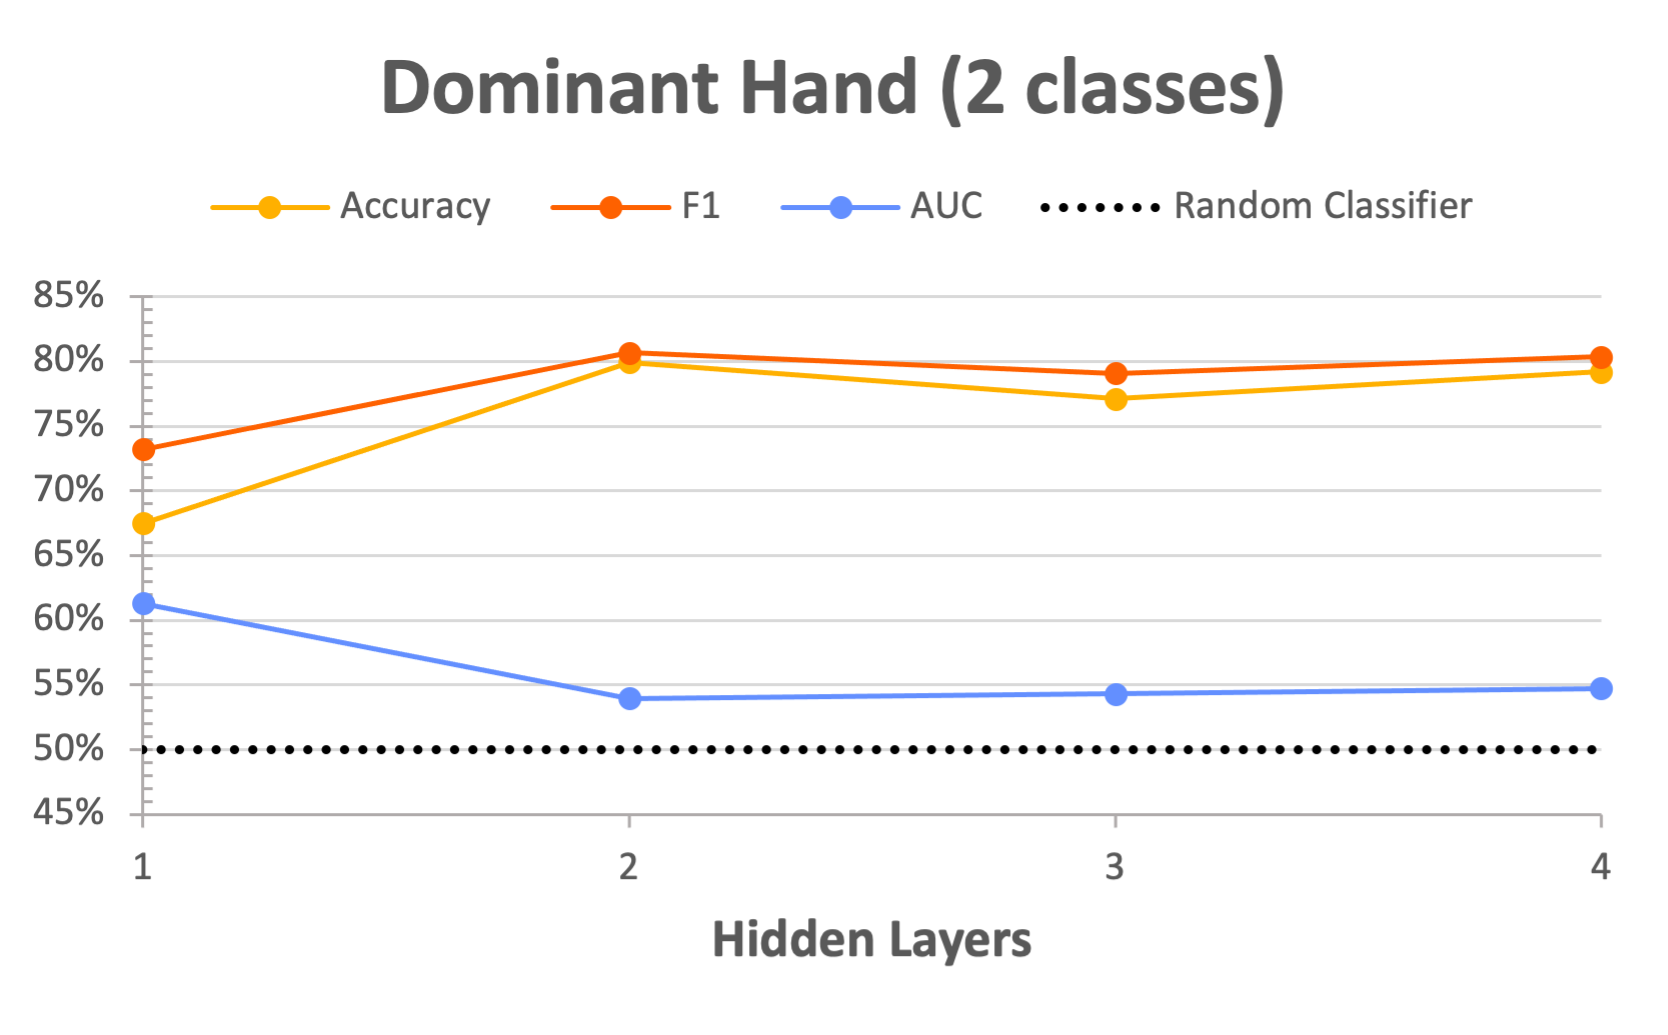
\includegraphics[width=\textwidth]{plots/layers_dom.png}
         \caption{Hidden Layers}
         \label{fig:layers_dom}
     \end{subfigure}
     \hfill
     \begin{subfigure}{\w}
         \centering
         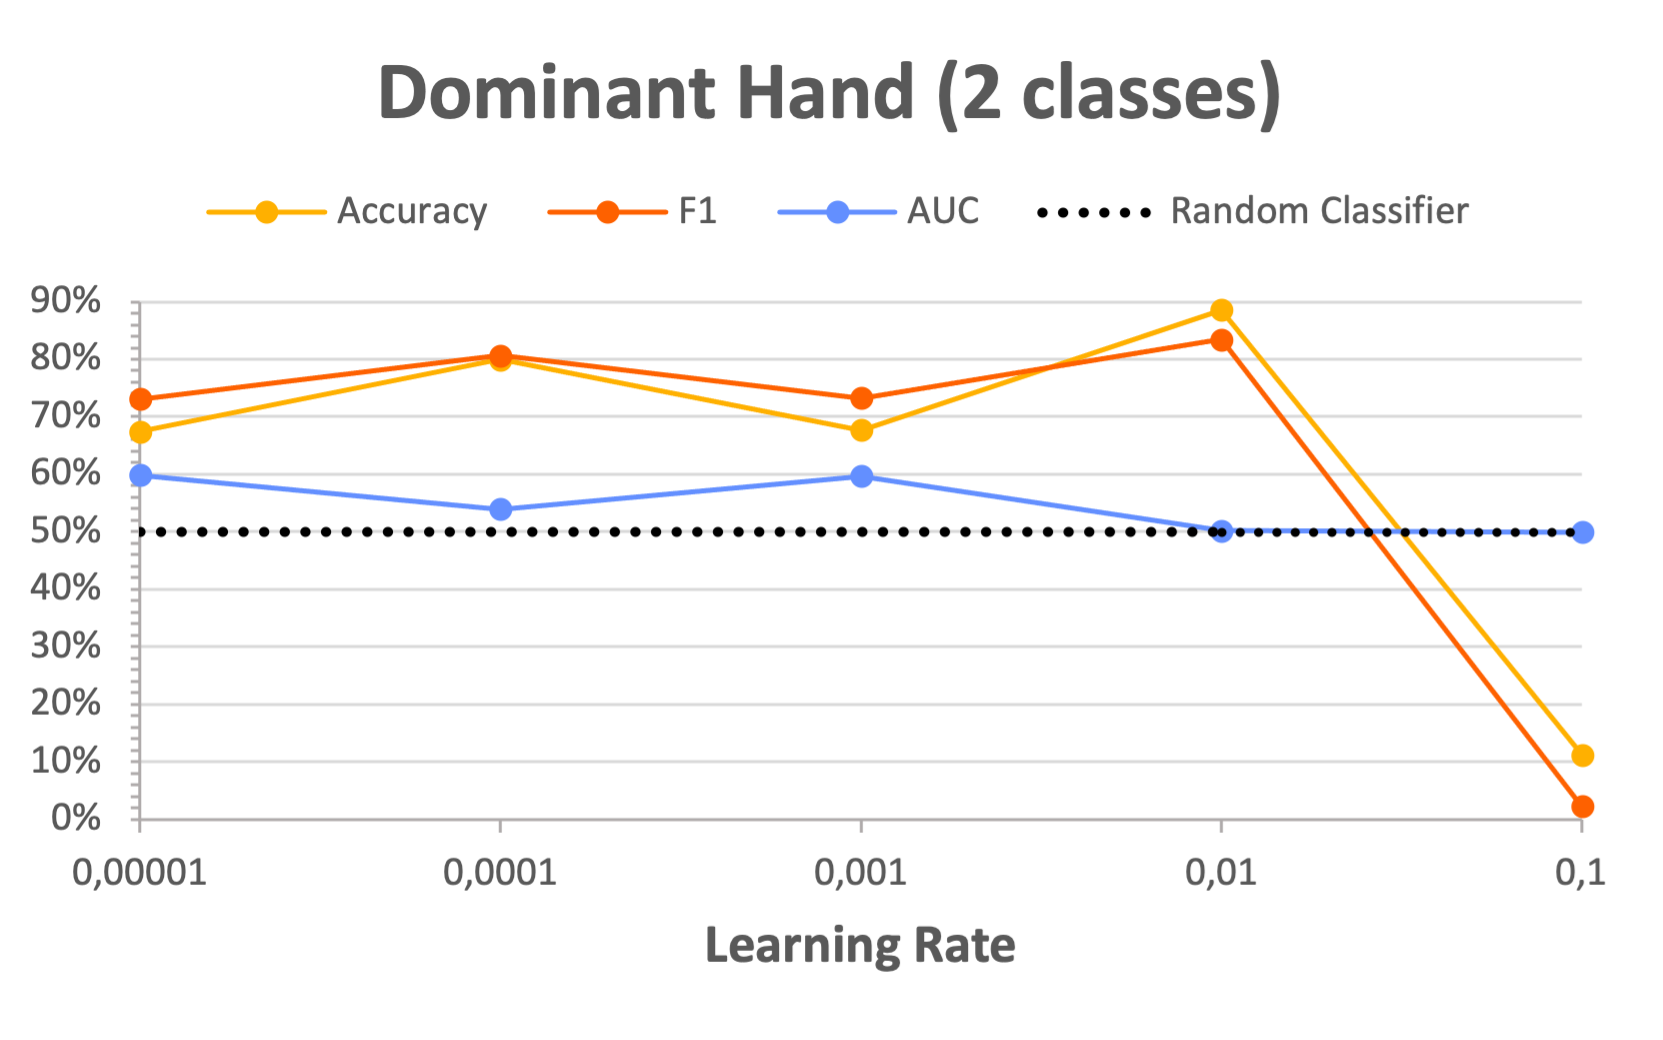
\includegraphics[width=\textwidth]{plots/lr_dom.png}
         \caption{Learning Rate}
         \label{fig:lr_dom}
     \end{subfigure}

    \caption{Predicting the user's dominant hand from swiped words trajectories.}
    \label{fig:dom}
\end{figure}

\begin{figure}[]
     \centering
     \def\w{0.45\linewidth}
     \begin{subfigure}{\w}
         \centering
         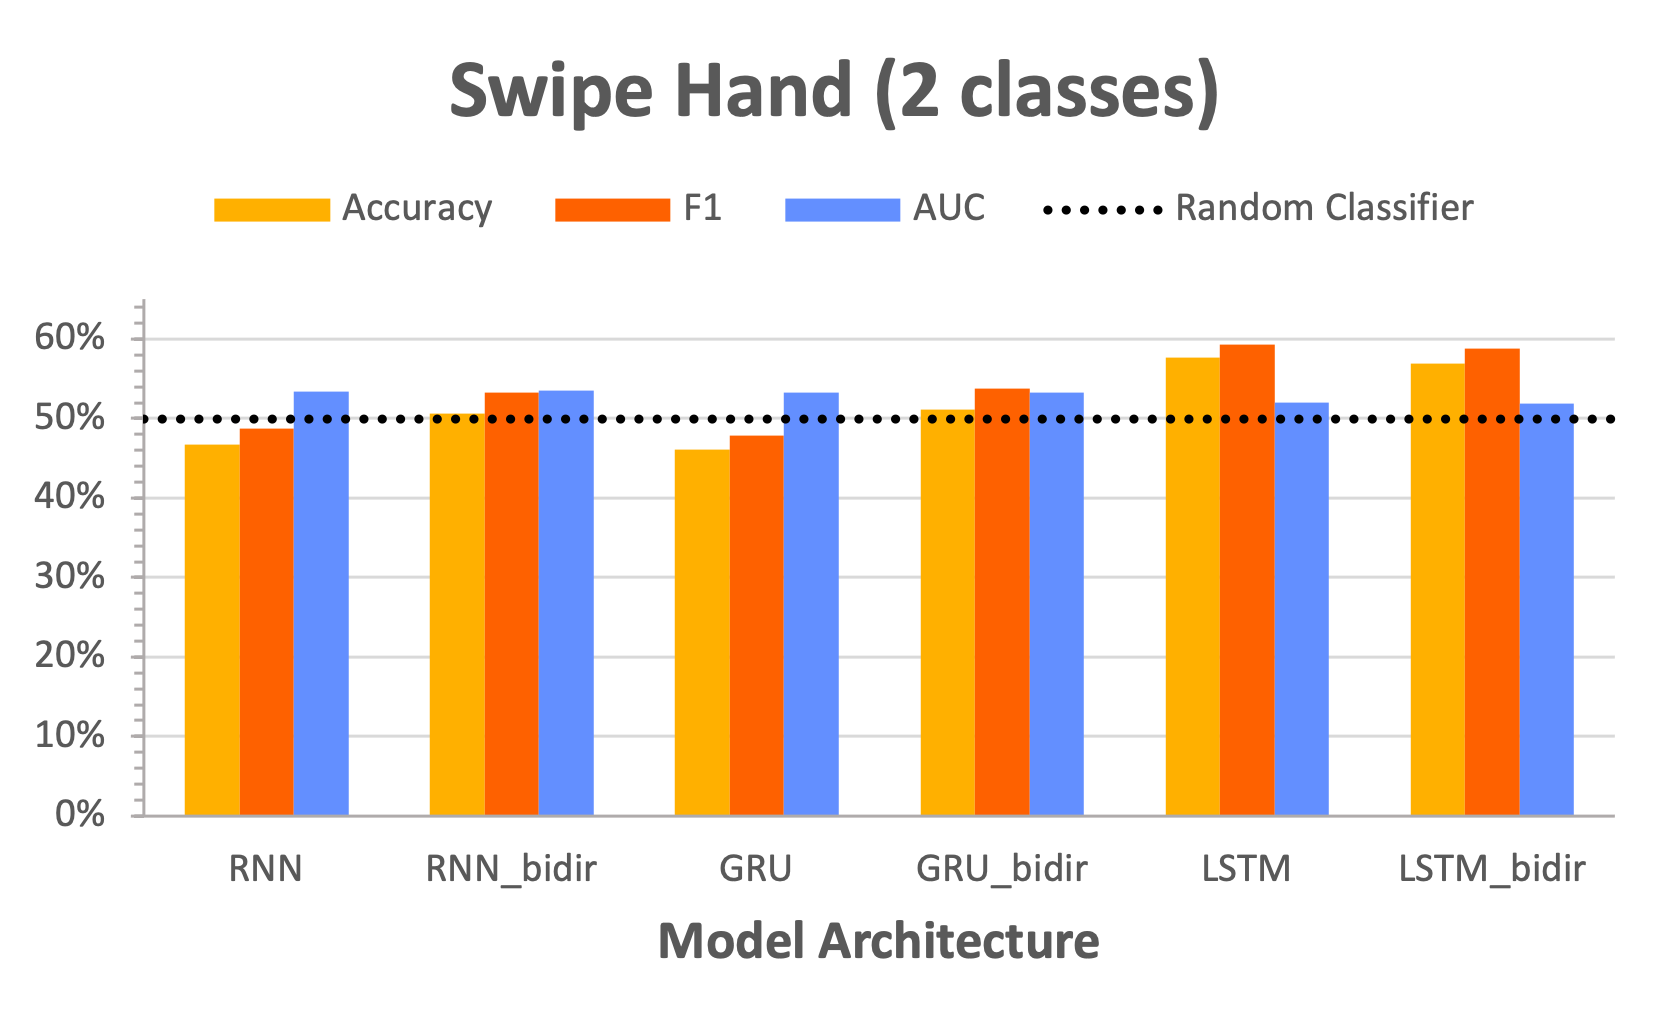
\includegraphics[width=\textwidth]{plots/model_hand.png}
         \caption{Layer type}
         \label{fig:models_hand}
     \end{subfigure}
     \hfill
     \begin{subfigure}{\w}
         \centering
         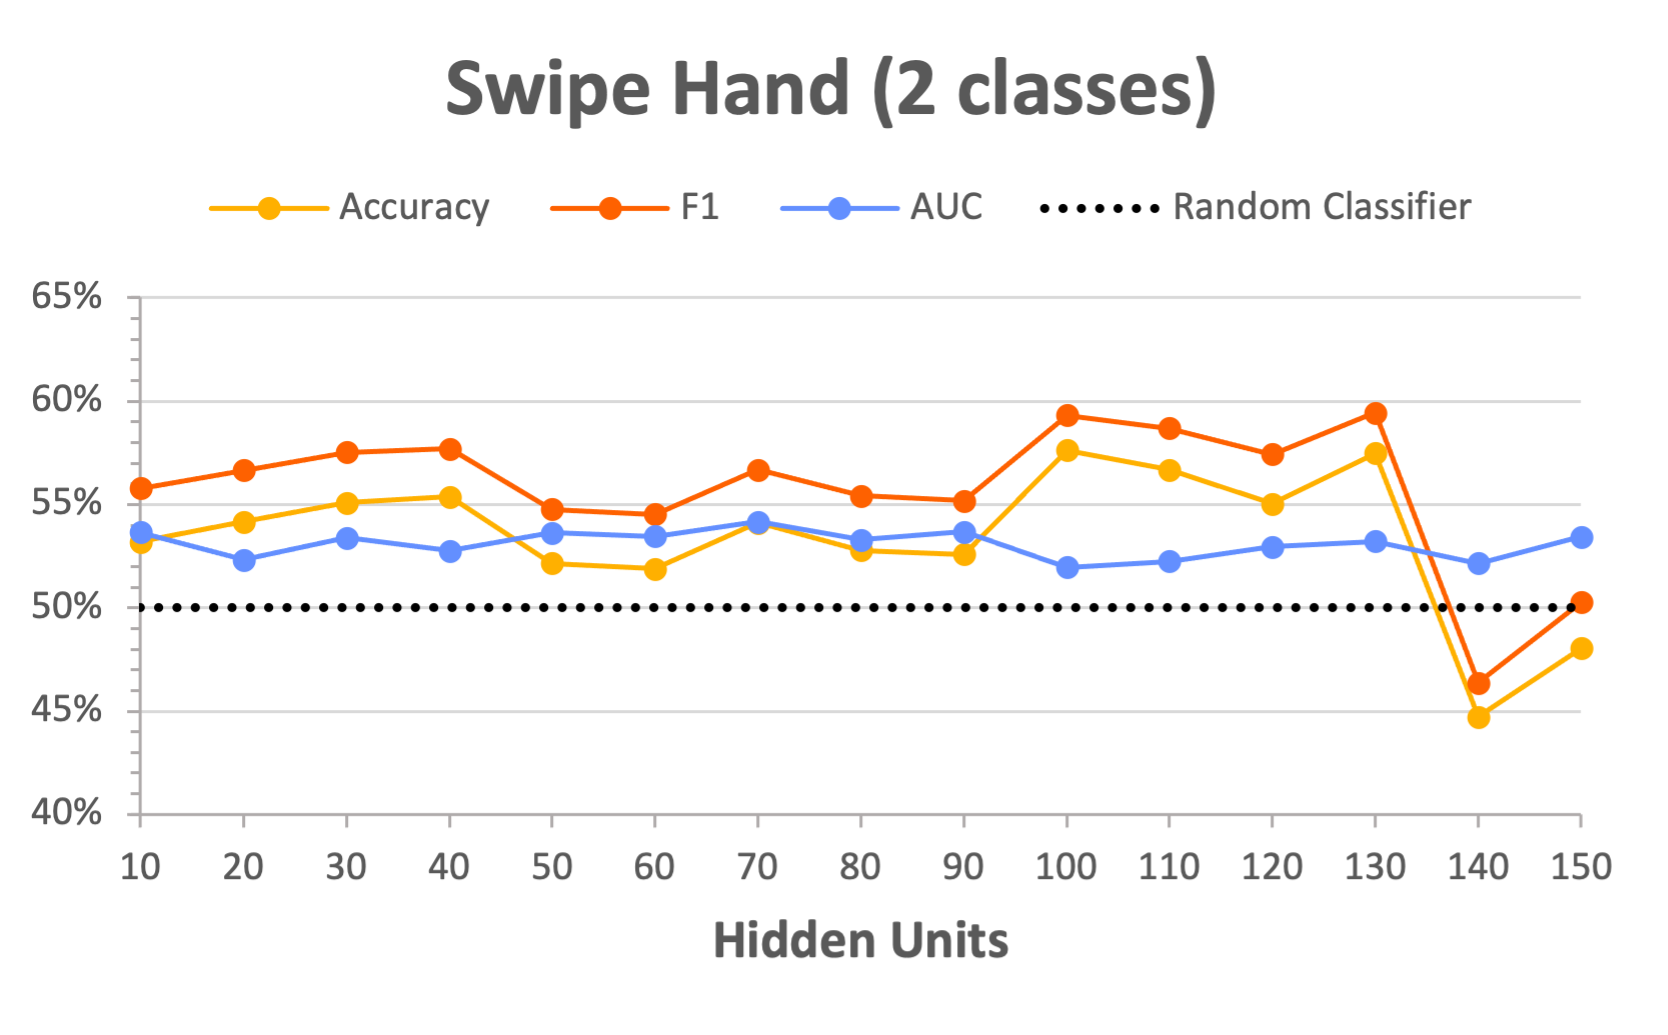
\includegraphics[width=\textwidth]{plots/units_hand.png}
         \caption{Hidden Units}
         \label{fig:units_hand}
     \end{subfigure}\\
     \begin{subfigure}{\w}
         \centering
         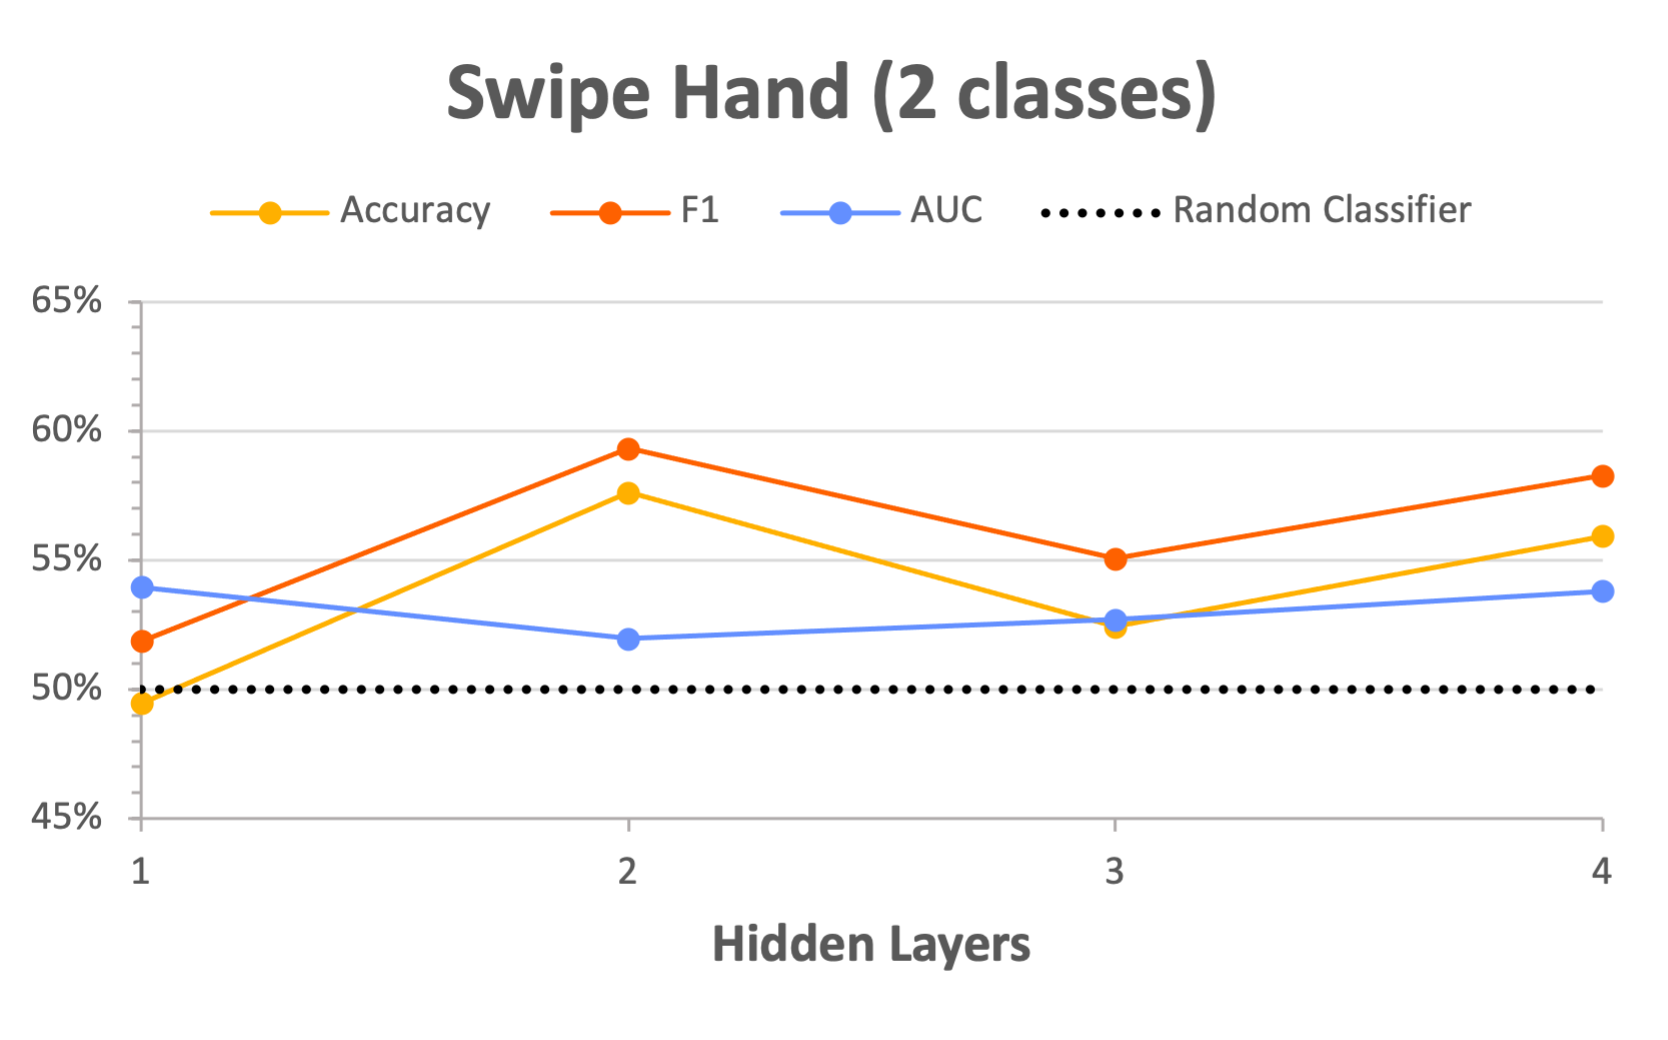
\includegraphics[width=\textwidth]{plots/layers_hand.png}
         \caption{Hidden Layers}
         \label{fig:layers_hand}
     \end{subfigure}
     \hfill
     \begin{subfigure}{\w}
         \centering
         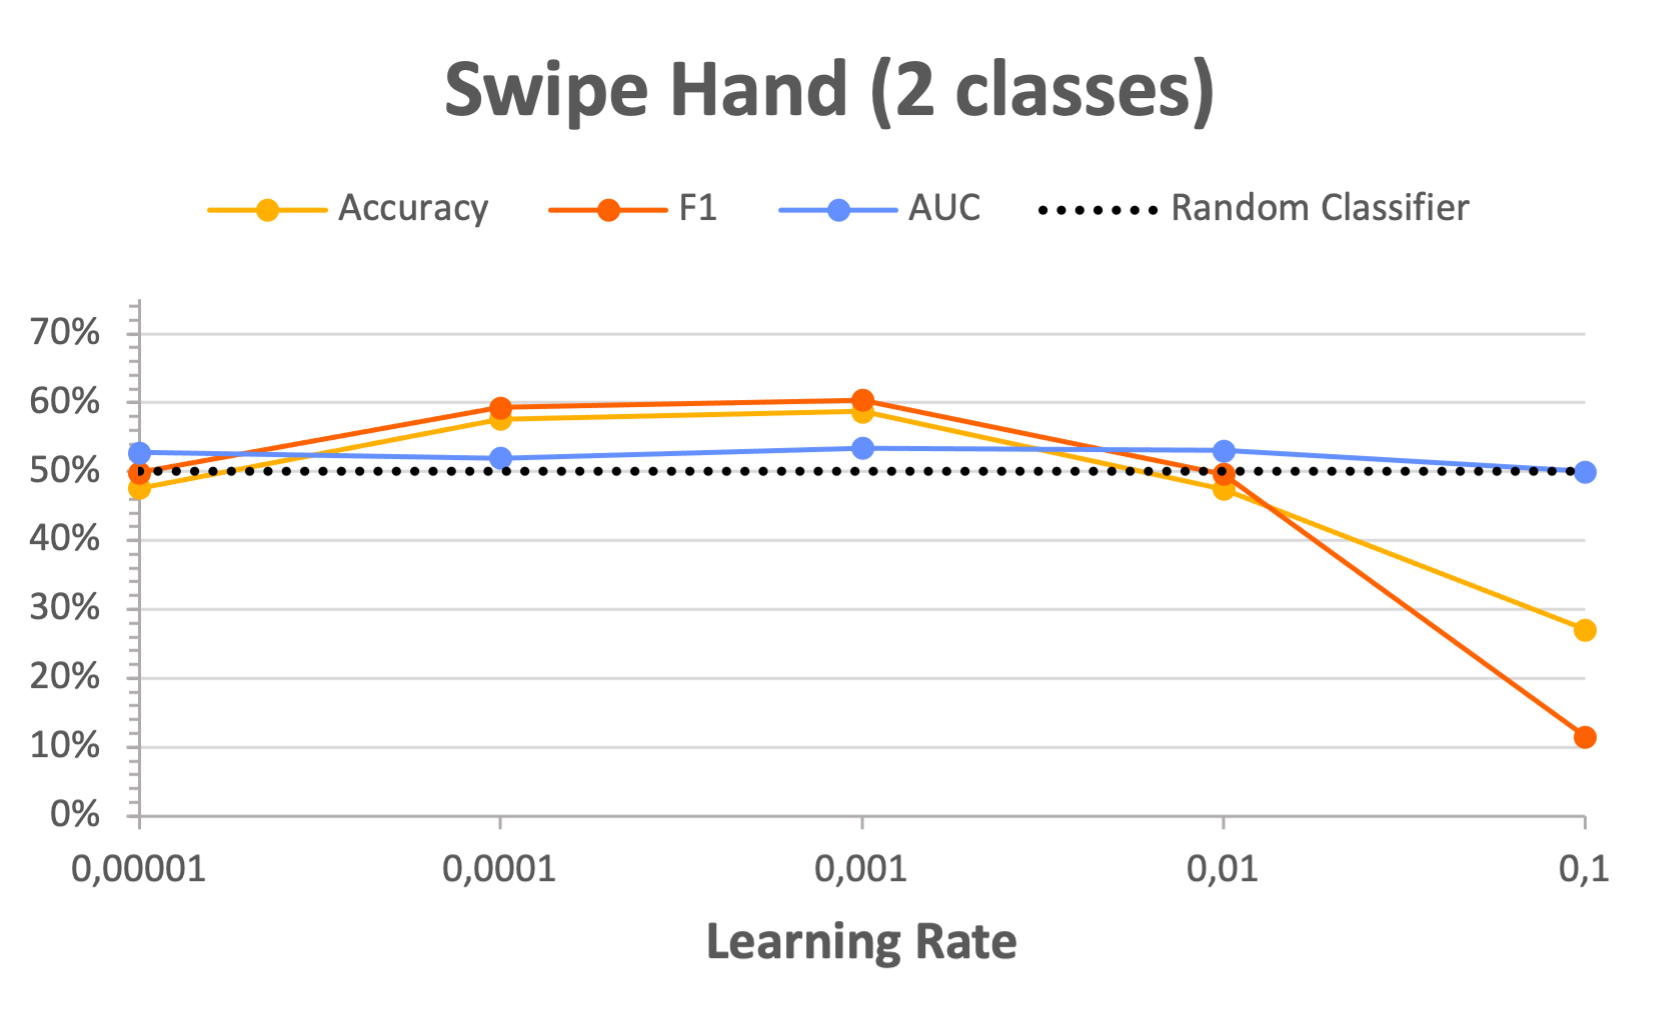
\includegraphics[width=\textwidth]{plots/lr_hand.png}
         \caption{Learning Rate}
         \label{fig:lr_hand}
     \end{subfigure}

    \caption{Predicting the user's swiping hand from swiped words trajectories.}
    \label{fig:hand}
\end{figure}

\begin{figure}[]
     \centering
     \def\w{0.45\linewidth}
     \begin{subfigure}{\w}
         \centering
         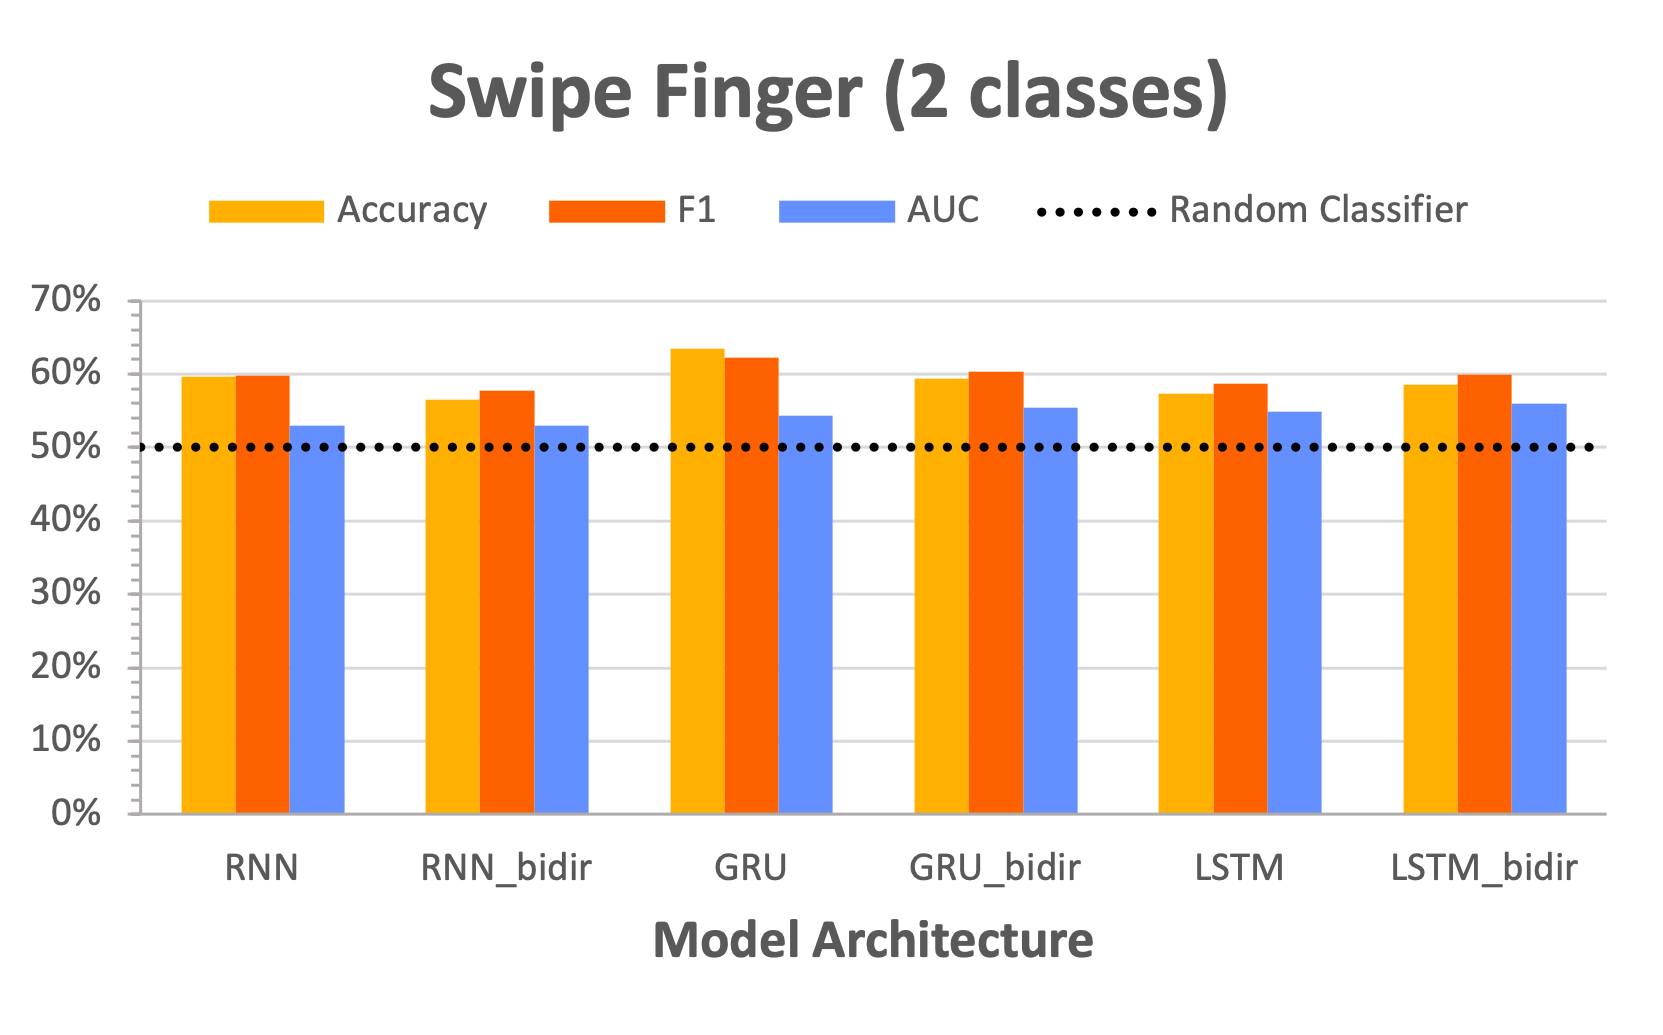
\includegraphics[width=\textwidth]{plots/model_finger.png}
         \caption{Layer type}
         \label{fig:models_finger}
     \end{subfigure}
     \hfill
     \begin{subfigure}{\w}
         \centering
         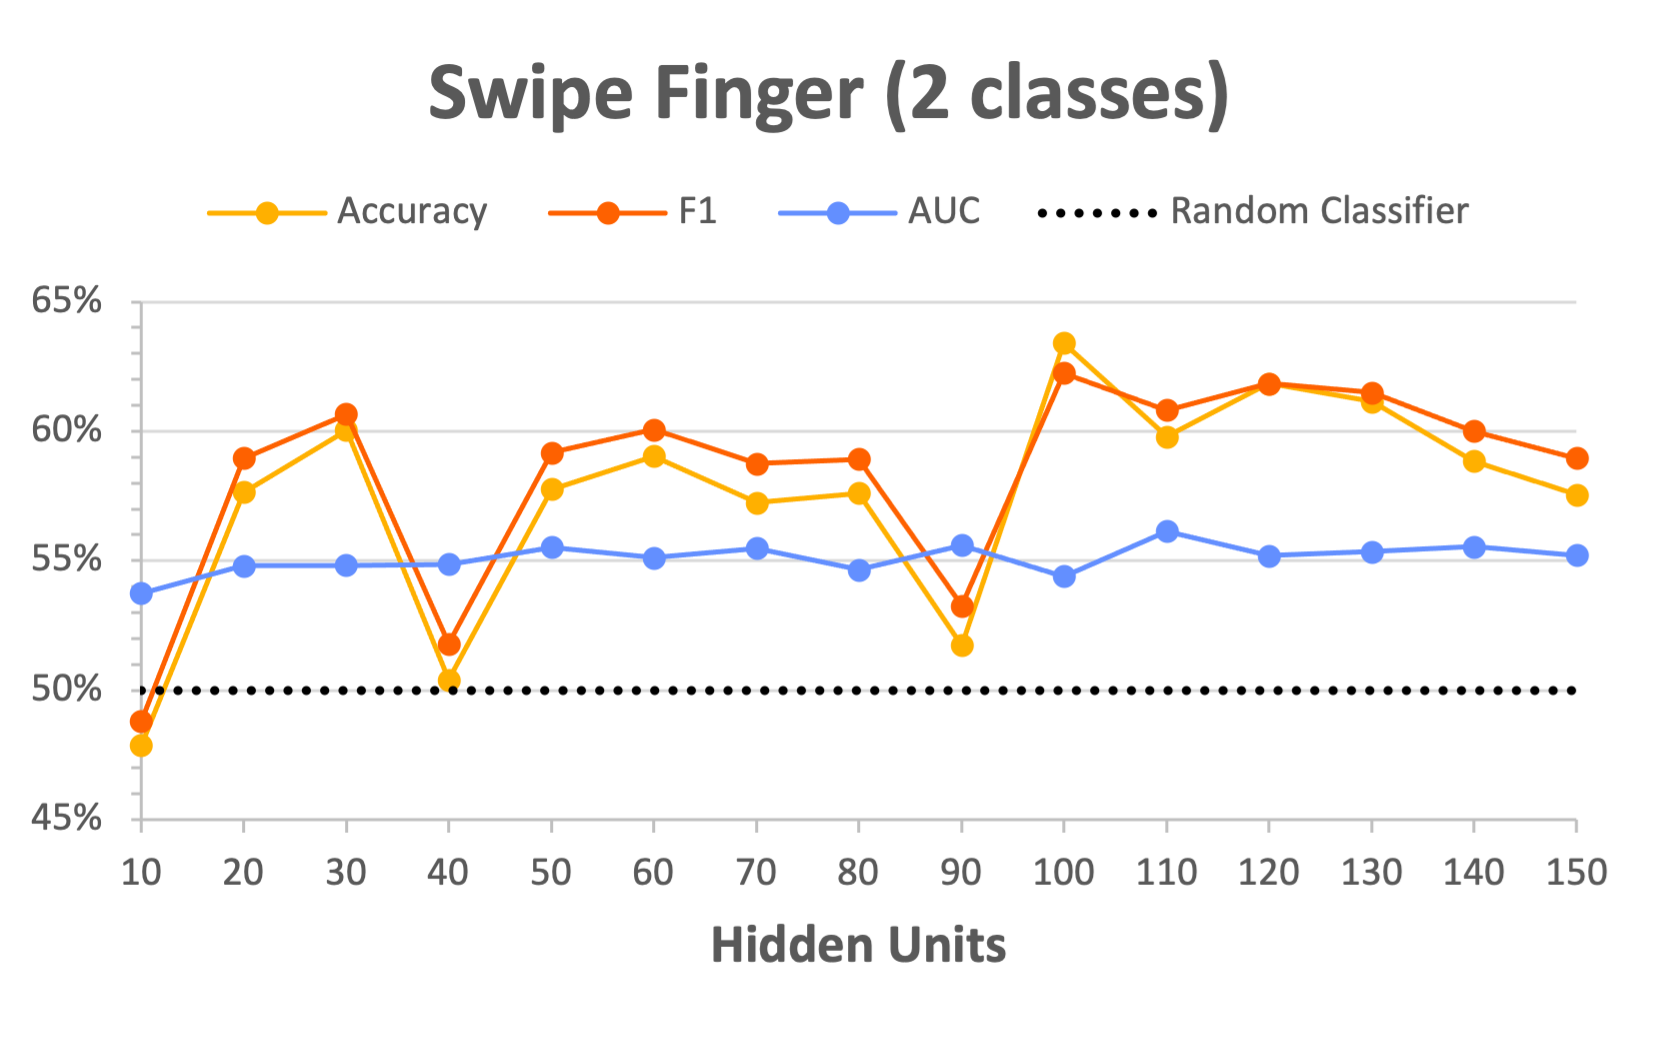
\includegraphics[width=\textwidth]{plots/units_finger.png}
         \caption{Hidden Units}
         \label{fig:units_finger}
     \end{subfigure}\\
     \begin{subfigure}{\w}
         \centering
         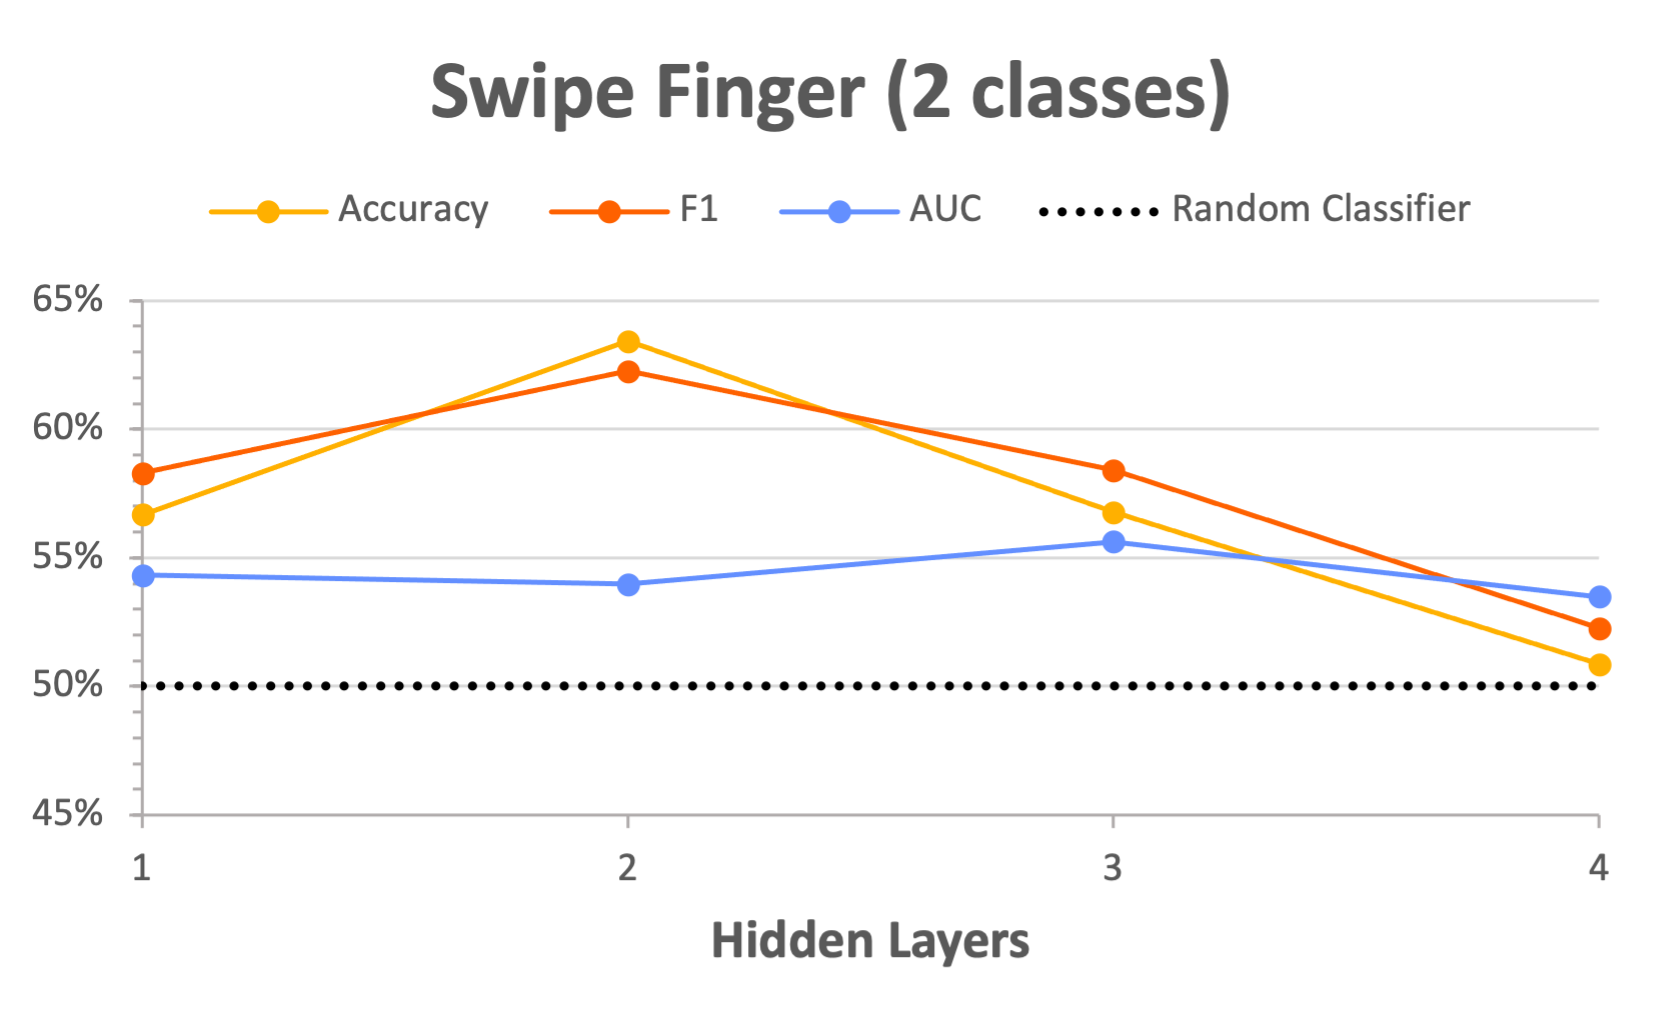
\includegraphics[width=\textwidth]{plots/layers_finger.png}
         \caption{Hidden Layers}
         \label{fig:layers_finger}
     \end{subfigure}
     \hfill
     \begin{subfigure}{\w}
         \centering
         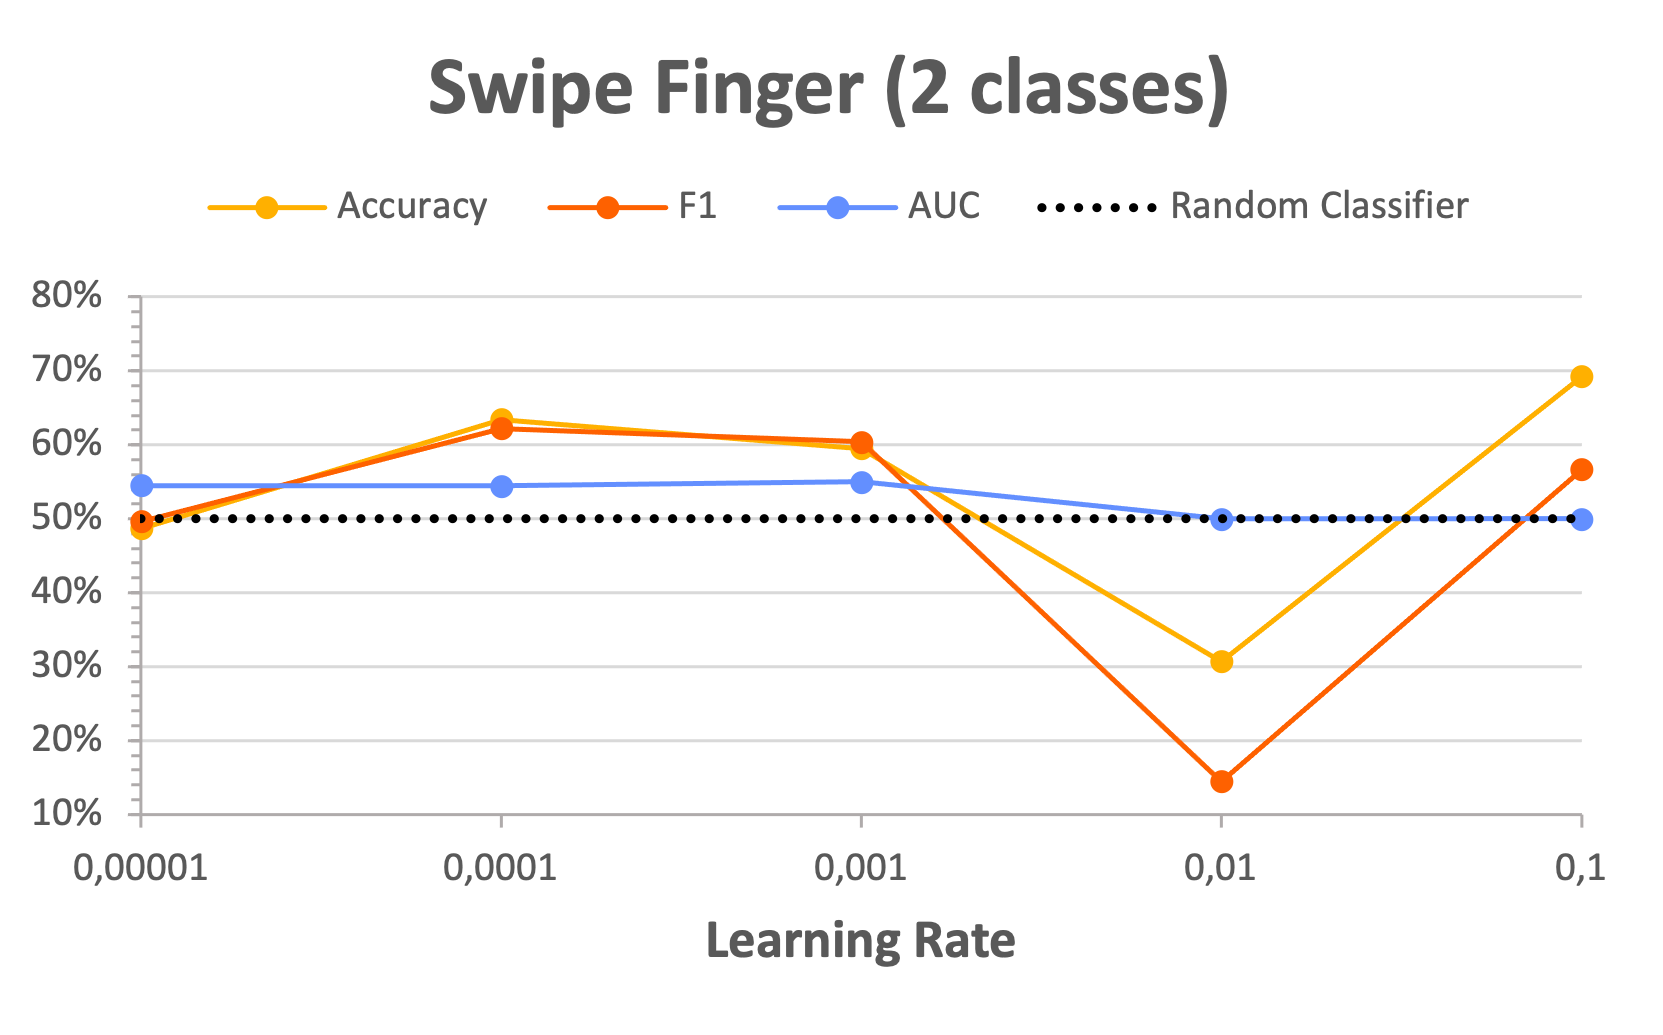
\includegraphics[width=\textwidth]{plots/lr_finger.png}
         \caption{Learning Rate}
         \label{fig:lr_finger}
     \end{subfigure}

    \caption{Predicting the user's swiping finger from swiped words trajectories.}
    \label{fig:finger}
\end{figure}
\vspace{1cm}
%For the swiping familiarity target in \autoref{fig:fam}, we have 3 classes such that a random classifier's accuracy is 33,33\%. The best performance accuracy is 37,87\%  with a non-bidirectional LSTM model with 2 hidden layers, 140 hidden units and 10$^{-4}$ learning rate. The performance is better than the one of the random classifier, which means that the model is able to learn some patterns about the swiping familiarity from the swiping trajectories. The worst performance accuracy is 26,23\% with a non-bidirectional LSTM model with 2 hidden layer, 20 hidden units and 10$^{-4}$ learning rate.\\

%For the English level target in \autoref{fig:engl}, we have 4 classes such that a random classifier's accuracy is 25\%. The best performance accuracy is 37,32\% with a bidirectional LSTM model with 4 hidden layers, 100 hidden units and 10$^{-4}$ learning rate. The performance is better than the one of the random classifier, which means that the model is able to learn some patterns about the English level from the swiping trajectories. The worst performance accuracy is 24,19\% with a bidirectional LSTM model with 4 hidden layers, 100 hidden units and 10$^{-1}$ or 10$^{-2}$ learning rates.\\

%For the age target in \autoref{fig:age}, we have 3 classes such that a random classifier's accuracy is 33,33\%. The best performance accuracy is 40,91\% with a bidirectional GRU model with 2 hidden layers, 150 hidden units and 10$^{-3}$ learning rate. The performance is better than the one of the random classifier, which means that the model is able to learn some patterns about the age from the swiping trajectories. The worst performance accuracy is 32,42\% with a bidirectional GRU model with 2 hidden layers, 150 hidden units and 10$^{-2}$ learning rate.\\

%For the nationality target in \autoref{fig:nat}, we have 2 classes such that a random classifier's accuracy is 50\%. The best performance accuracy is 63,50\% with a non-bidirectional RNN model with 2 hidden layers, 150 hidden units and 10$^{-4}$ learning rate. The performance is better than the one of the random classifier, which means that the model is able to learn some patterns about the nationality from the swiping trajectories. The worst performance accuracy is 38,85\% with a non-bidirectional RNN model with 2 hidden layers, 150 hidden units and 10$^{-1}$ or 10$^{-2}$ learning rates.\\

%For the gender target in \autoref{fig:gender}, we have 2 classes such that a random classifier's accuracy is 50\%. The best performance accuracy is 68,51\% with a bidirectional LSTM model with 2 hidden layers, 50 hidden units and 10$^{-1}$ learning rate. The performance is better than the one of the random classifier, which means that the model is able to learn some patterns about the gender from the swiping trajectories. The worst performance accuracy is 51,85\% with a bidirectional LSTM model with 2 hidden layers, 50 hidden units and 10$^{-5}$ learning rate.\\

%For the dominant hand target in \autoref{fig:dom}, we have 2 classes such that a random classifier's accuracy is 50\%. The best performance accuracy is 88,57\% with a bidirectional LSTM model with 2 hidden layers, 150 hidden units and 10$^{-2}$ learning rate. The performance is better than the one of the random classifier, which means that the model is able to learn some patterns about the dominant hand from the swiping trajectories. The worst performance accuracy is 11,29\% with a bidirectional LSTM model with 2 hidden layers, 150 hidden units and 10$^{-1}$ learning rate.\\

%For the swiping hand target in \autoref{fig:hand}, we have 2 classes such that a random classifier's accuracy is 50\%. The best performance accuracy is 58,74\% with a non-bidirectional LSTM model with 2 hidden layers, 100 hidden units and 10$^{-3}$ learning rate. The performance is better than the one of the random classifier, which means that the model is able to learn some patterns about the swiping hand from the swiping trajectories. The worst performance accuracy is 27,08\% with a non-bidirectional LSTM model with 2 hidden layers, 100 hidden units and 10$^{-1}$ learning rate.\\

%For the swiping finger target in \autoref{fig:finger}, we have 2 classes such that a random classifier's accuracy is 50\%. The best performance accuracy is 69,28\% with a non-bidirectional GRU model with 2 hidden layers, 100 hidden units and 10$^{-1}$ learning rate. The performance is better than the one of the random classifier, which means that the model is able to learn some patterns about the swiping finger from the swiping trajectories. The worst performance accuracy is 30,74\% with a non-bidirectional GRU model with 2 hidden layers, 100 hidden units and 10$^{-2}$ learning rate.\\
\vspace{2cm}
\autoref{tab:results} summarizes the best performing models and their corresponding hyperparameters in comparison with that of a random classifier baseline. The classifiers performed best on most demographical and behavioural traits by defining the model to be bidirectional and choosing recurrent layers with LSTM or GRU cells. As we can see from the results table all models performed  better than a random classifier, with an increase from 4 to 10\% for the swiping familiarity, age and swiping hand targets, and with an increase from 10 to almost 40\% for the English level, nationality, gender, dominant hand and swiping finger targets. The dataset is more representative for some targets and results in higher performance.  Overall, this shows that the trained classifiers were able to identify latent demographic traits from the swiping trajectories. Hence, validating our hypothesis that swiping carries rich information about user demographic and behavioural traits, which opens an interesting research avenue which is yet to be explored.


\newline
\begin{table}[]
\centering
\resizebox{\columnwidth}{!}{%
\begin{tabular}{||l|c|c|c|c|c|l||}
\hline
Target &
  \multicolumn{1}{l|}{Model} &
  \multicolumn{1}{l|}{Hidden layers} &
  \multicolumn{1}{l|}{Hidden units} &
  \multicolumn{1}{l|}{Learning rate} &
  \begin{tabular}[c]{@{}c@{}}Random classifier\\ accuracy\end{tabular} &
  Model accuracy \\ \hline
\textbf{Swiping familiarity} & LSTM   & 2 & 140 & 10^{-4} & \textbf{33.33\%} & \textbf{37.87\%} \\ \hline
\textbf{English level}       & BiLSTM & 4 & 100 & 10^{-4} & \textbf{25\%}    & \textbf{37.32\%} \\ \hline
\textbf{Age}                 & BiGRU  & 2 & 150 & 10^{-3} & \textbf{33.33\%} & \textbf{40.91\%} \\ \hline
\textbf{Nationality}         & RNN    & 2 & 150 & 10^{-4} & \textbf{50\%}    & \textbf{63.50\%}   \\ \hline
\textbf{Gender}              & BiLSTM & 2 & 50  & 10^{-1} & \textbf{50\%}    & \textbf{68.51\%} \\ \hline
\textbf{Dominant hand}       & BiLSTM & 2 & 150 & 10^{-2} & \textbf{50\%}    & \textbf{88.57\%} \\ \hline
\textbf{Swiping hand}        & LSTM   & 2 & 100 & 10^{-3} & \textbf{50\%}    & \textbf{58.74\%} \\ \hline
\textbf{Swiping finger}      & GRU    & 2 & 100 & 10^{-1} & \textbf{50\%}    & \textbf{69.28\%} \\ \hline
\end{tabular}%
}
\caption{Results}
\label{tab:results}
\end{table}\newline





%% ============================================================================
\chapter{Limitations and Future Work}
%% ============================================================================

%% Provide a high-level discussion of the results?
%% What have we learned?
%% What is the takeaway message?
%% What are the limitations of our study?
%% What should be done in the future?
Sequence models typically require a huge amount of data to achieve a good discriminative power. Nevertheless, we trained our sequential models on limited dataset of 81,175 swiping trajectories, filtering out only the correctly swiped words from around one thousand users. Although the results obtained in our study are indicators for the presence of latent demographic and behavioural traits embedded within swiping data, these models need to be trained on a significantly larger swiping dataset to precisely identify latent demographic and behavioural traits.\\


%Sequence models typically require a huge amount of data to achive a good discriminative power Although the results obtained in our study are indicators for the presence of latent demofraphic and behavioural traits embedded within swiping data, The swiping dataset used in this study  We trained our sequential models based on limited swiping data from around one thousand users. We had only around eighty-one thousand swiping data by filtering out only the correctly swiped words.The performances of our models are affected by the limited data resources. Sequence models require normally a huge amount of data to predict very precisely. Thus, the data limitation was a challenge and our models were not performing amazing for most targets but still good. If our dataset would have consisted of more than one million swiping trajectories then our models would have predicted the different features extremely precise.\\


%Firstly, we always tested in our experiments which model architecture, e.g. RNN, BiRNN, GRU, BiGRU, LSTM and BiLSTM, performed best. We conducted for 5 features 21 experiments with  either a bidirectional LSTM or GRU model, i.e. very long training times due to the model type choices already. Thus, we run


In this work we focused on single-word classification,
which is the most challenging scenario since some words might be as short as two characters
and therefore the information a classifier can infer is minimal.
It would be interesting to predict demographical and behavioral attributes
at the sentence level, i.e., by considering all swiped words a user might enter in row.
This could be done by concatenating the feature vectors of each word in the sentence.
We have not considered word difficulty in our analysis.
This might be an interesting avenue for future work,
since it has been shown that experienced shape-writing users
tend to be more loose while entering non-familiar words~\cite{Leiva21_swipe}.
It may be the case, therefore, that other behavioral and biometric traits
are highly correlated with swiping patterns.
For example, ageing is marked by a decline in motor control abilities, which is reflected by the users' writing performance.
Smith et al.~\cite{Smith1999} observed that older people incurred in longer movement times,
but also more sub-movements and more pointing errors than the young.
Unfortunately, we cannot study this effect in the dataset we have analyzed,
since most users are aged between 20 and 40 years.
More concretely, the dataset is skewed towards young female right-handed participants from the US.\\

Furthermore, in our study we leveraged the sequence of trajectories and explored only sequential models, RNN, LSTM and GRU as they are better suited to handle the sequential nature of trajectories. Observing the promising results obtained in our study we believe that leveraging images of swipe trajectories, other architectures such as Convolutional Neural Networks (CNNs) as well as more powerful ones like vision transformers can be explored in the future for a potentially better performance.\\\newpage

Nowadays, mobile vendors provide  the swiping service to millions of users.  Although, they ask for consent to track swiping information for the purpose of improving the service and enhancing user experience, our study brings to light that extracting personal information of users from swiping data is also within reach. The significantly large amount of swiping data mobile vendors can have access to, allows them to build a powerful demographic and behavioral inference engines. Thus, the users can potentially give up their privacy, without actually consenting to it, only by sharing their swiping information with mobile vendors. \\

%% ============================================================================
\chapter{Conclusion}
%% ============================================================================
%% Summarize in 1 or 2 paragraphs this work.
%% Restate again (but briefly) the main contributions.
%% Conclude with a sentence that provides a broader perspective of this work.
This work explores Shape-writing also known as gesture typing or swiping which is a word-based text entry method for touchscreen keyboards. It works by landing the finger on (or close to) the first character of the desired word  and then sliding over all the other character keys without lifting the finger until the last word character is reached.  This generates a trajectory of swiped characters on the keyboard layout which can be translated to a meaningful word by a statistical decoder. Today this service is offered by all mobile vendors and has millions of users. Nevertheless due to the lack of publicly available dataset  the topic of Shape-writing has not be sufficiently explored. \\

In this work we hypothesized that swiping carries rich information about the user,  such as demographical (e.g. age or gender) and behavioral (e.g. swiping familiarity or input finger) information. Hence,  we analyzed the dynamics of swiping trajectories from the only publicly available swiping dataset to model and predict different demographical and behavioural traits.  We leveraged  the sequence of swiping trajectories from the dataset in order to train sequence models that can discriminate demographical and behavioural traits of users. In particular we explored 3 of the popular sequence model architectures (RNN, LSTM, GRU) and conducted a systematic analysis on which popular network architectures hyperparameters yield better performance.  (i.e., the type of layer(RNN, LSTM or GRU), if bidirectional or not, the number of hidden neurons, the number of hidden layers and the learning rate).  The classifiers performed best on most demographical and behavioural traits by defining the model to be bidirectional and choosing recurrent layers with LSTM or GRU cells. \\

The results from our experimental evaluations demonstrate that  all models performed better than a random classifier, with an increase from 4 to 10\% for the swiping familiarity, age and swiping hand targets, and with an increase from 10 to almost 40\% for the english level, nationality, gender, dominant hand and swiping finger targets. The dataset was found to be more representative for some targets and results in higher performance. Although the  performances of our models were encumbered by the small size of the dataset, overall the reported results show that the classifiers were able to identify latent demographic traits from the swiping trajectories. Hence, validating our hypothesis that swiping carries rich information about user demographic and behavioural traits, opening an interesting research avenue which is yet to be explored. To this end, our work brings to light that the cognitive and motor control mechanisms are embodied and reflected in swipe trajectories,  and that user privacy may be at risk by unethical mobile vendors or fishy soft keyboards.




\addcontentsline{toc}{chapter}{Bibliography}
\bibliographystyle{abbrv}
\bibliography{references.bib}
\newpage


\appendix
\chapter{Swiping Familiarity - Experiment Results Tables}\label{appendix:app_fam}
\addcontentsline{lot}{chapter}{Swiping Familiarity - Experiment Results Tables}
The experiment results for the different variations of model architectures, hidden units, hidden layers and learning rates are provided in this appendix for the swiping familiarity feature. The blue color indicates on which hyperparameter we experimented in each table. The best performance is colored green in all the individual tables.\\

\begin{table}[!ht]
\centerline{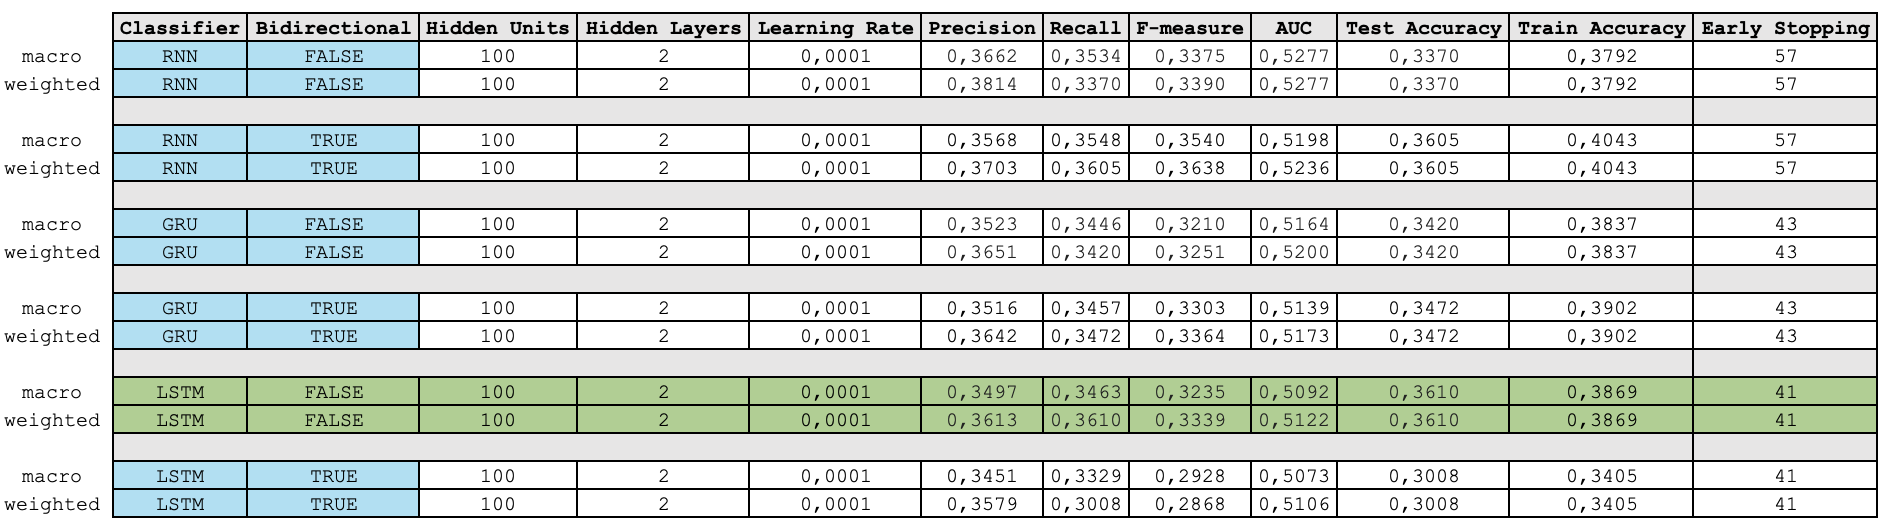
\includegraphics[width=1.2\linewidth]{appendix_tables/fam_models_table.png}}
\caption{Swiping Familiarity - Models Experiment Results}
\label{table:fam_models_table}
\end{table}

\begin{table}[!ht]
\centerline{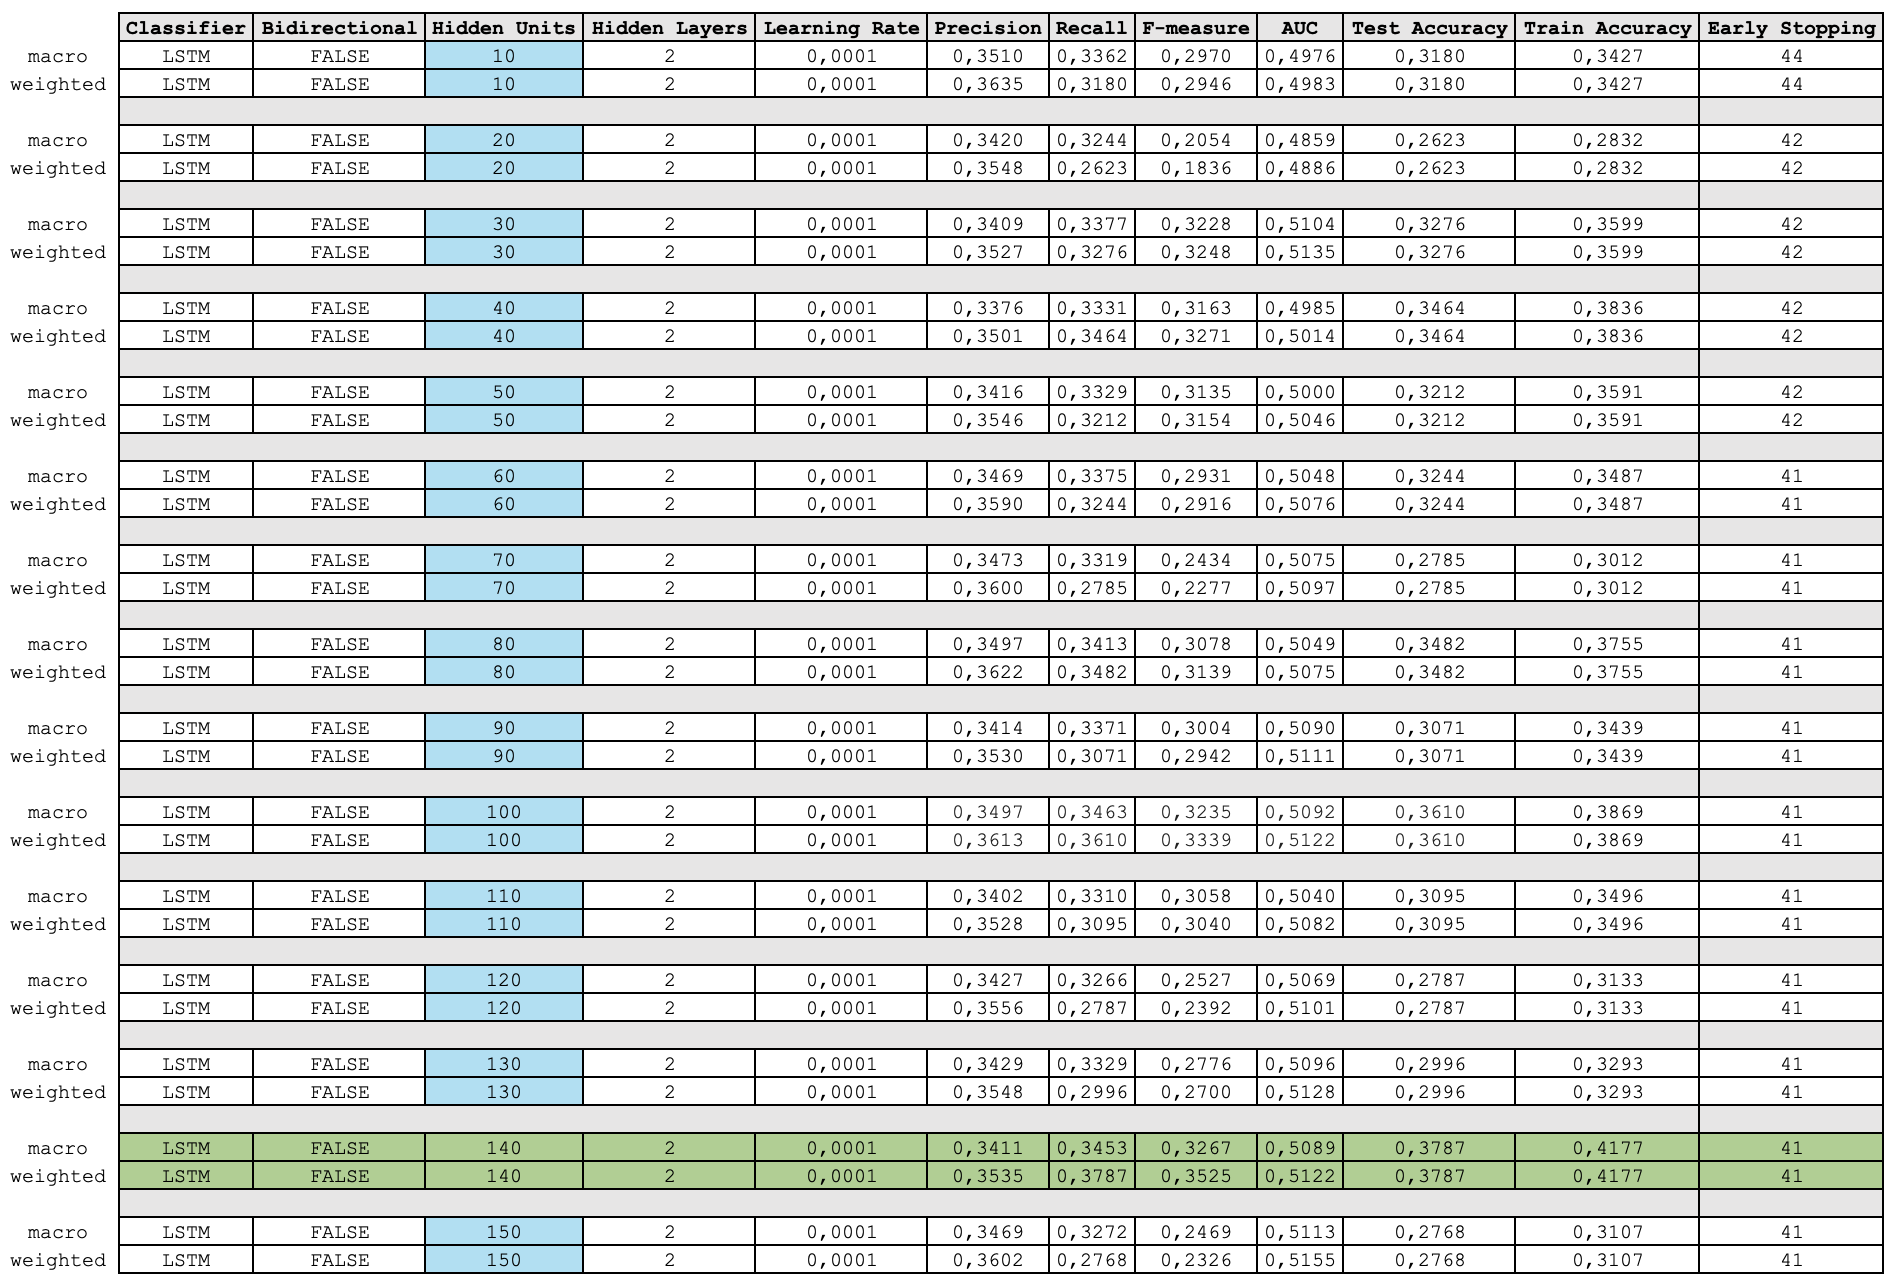
\includegraphics[width=1.2\linewidth]{appendix_tables/fam_units_table.png}}
\caption{Swiping Familiarity - Hidden Units Experiment Results}
\label{table:fam_units_table}
\end{table}

\begin{table}[!ht]
\centerline{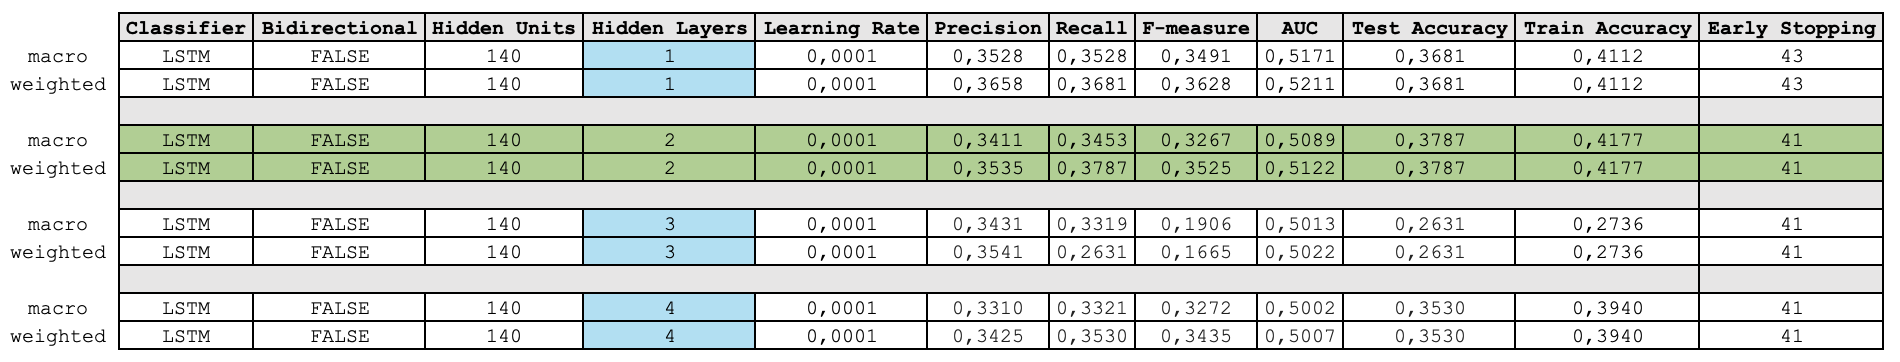
\includegraphics[width=1.2\linewidth]{appendix_tables/fam_layers_table.png}}
\caption{Swiping Familiarity - Hidden Layers Experiment Results}
\label{table:fam_layers_table}
\end{table}

\begin{table}[!ht]
\centerline{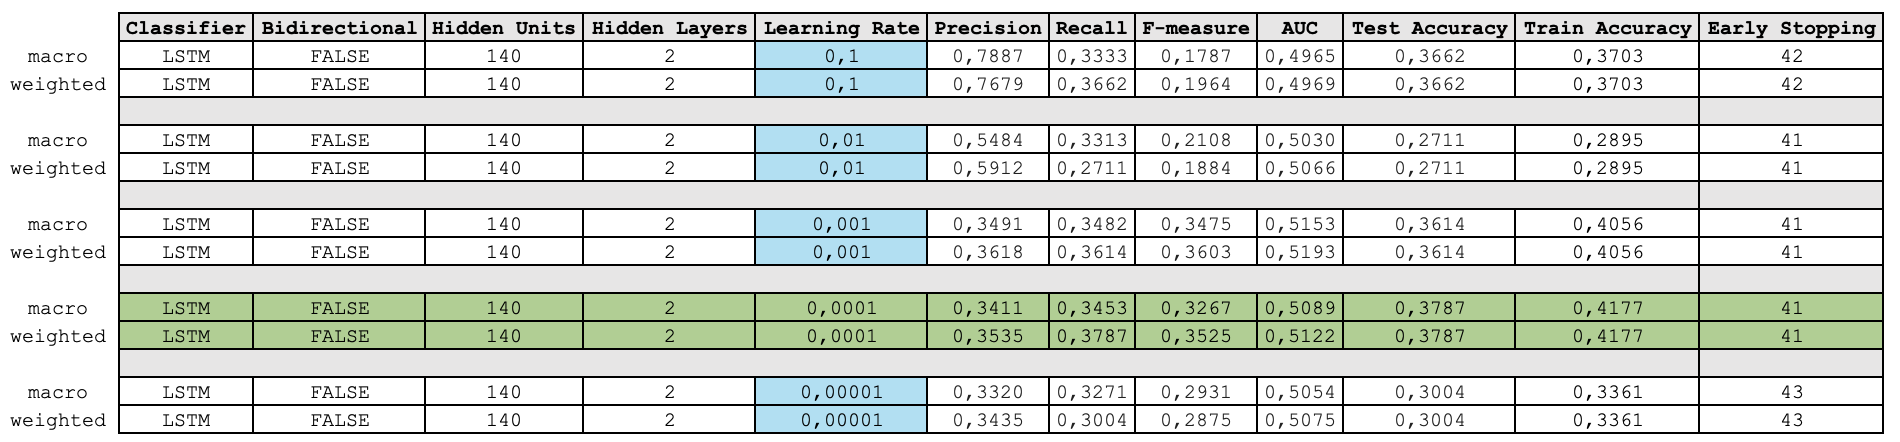
\includegraphics[width=1.2\linewidth]{appendix_tables/fam_lr_table.png}}
\caption{Swiping Familiarity - Learning Rate Experiment Results}
\label{table:fam_lr_table}
\end{table}




\chapter{English Level - Experiment Results Tables}\label{appendix:app_engl}
\addcontentsline{lot}{chapter}{English Level - Experiment Results Tables}
The experiment results for the different variations of model architectures, hidden units, hidden layers and learning rates are provided in this appendix for the English level feature. The blue color indicates on which hyperparameter we experimented in each table. The best performance is colored green in all the individual tables.\\

\begin{table}[!ht]
\centerline{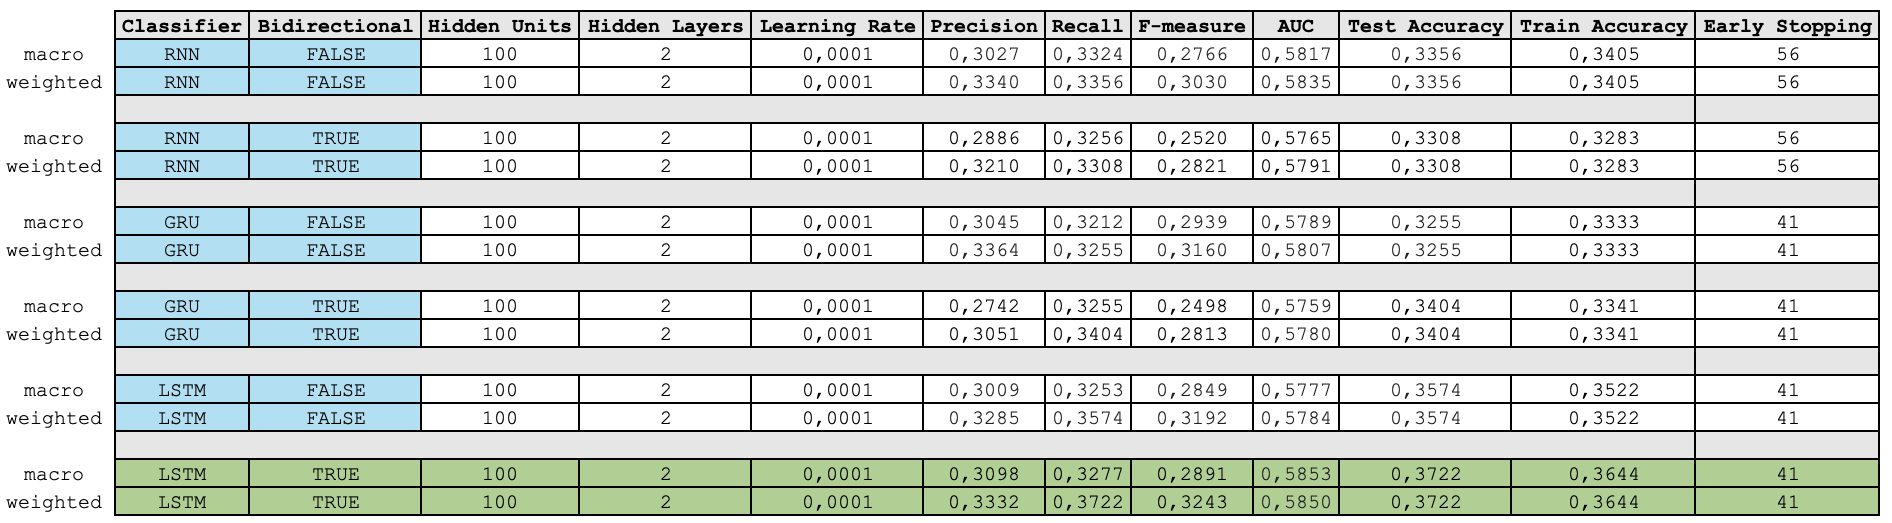
\includegraphics[width=1.2\linewidth]{appendix_tables/engl_models_table.png}}
\caption{English Level - Models Experiment Results}
\label{table:engl_models_table}
\end{table}

\begin{table}[!ht]
\centerline{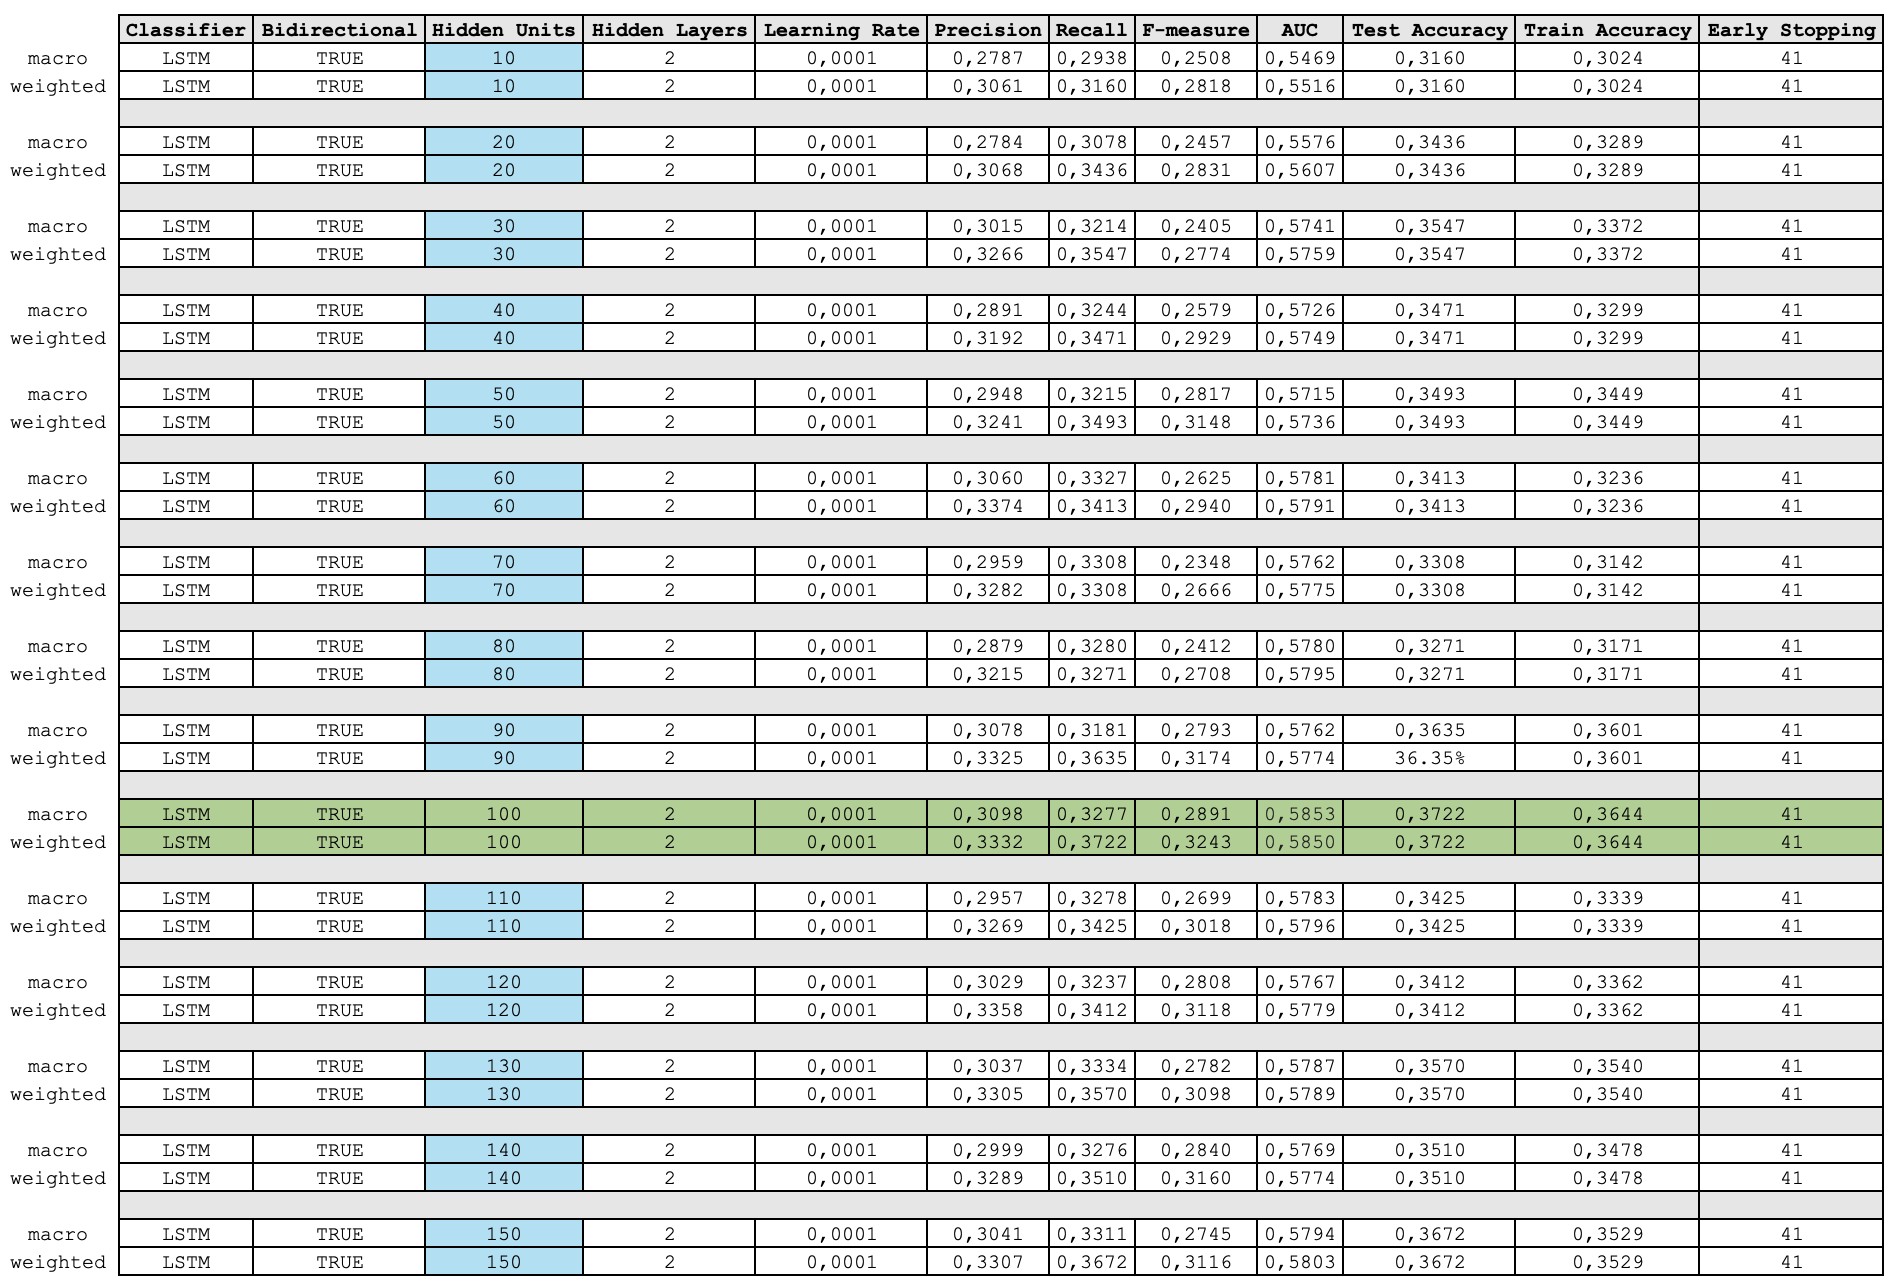
\includegraphics[width=1.2\linewidth]{appendix_tables/engl_units_table.png}}
\caption{English Level - Hidden Units Experiment Results}
\label{table:engl_units_table}
\end{table}

\begin{table}[!ht]
\centerline{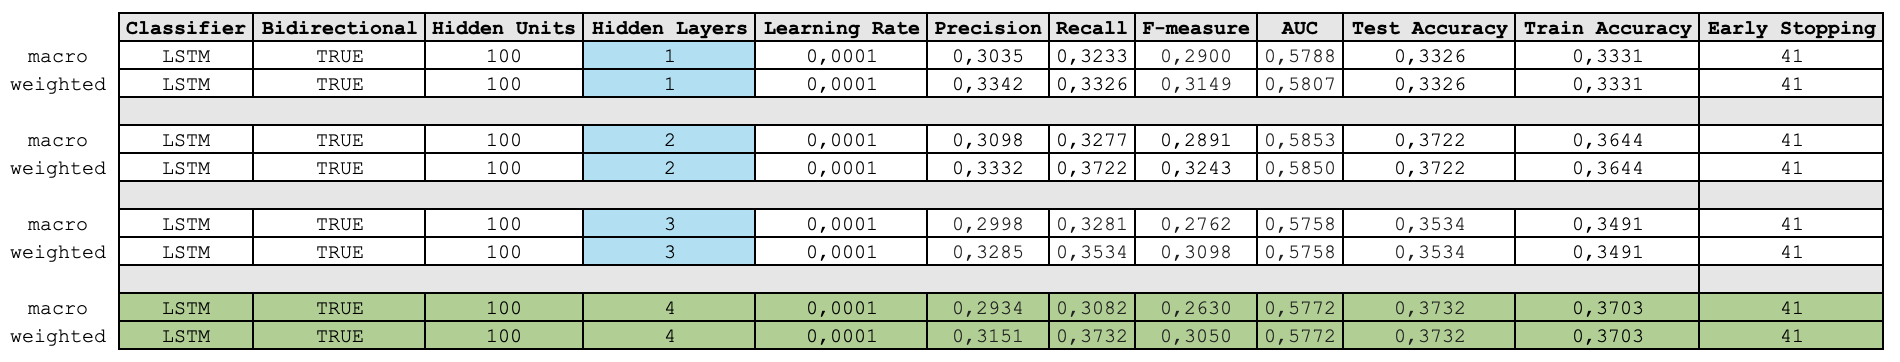
\includegraphics[width=1.2\linewidth]{appendix_tables/engl_layers_table.png}}
\caption{English Level - Hidden Layers Experiment Results}
\label{table:engl_layers_table}
\end{table}

\begin{table}[!ht]
\centerline{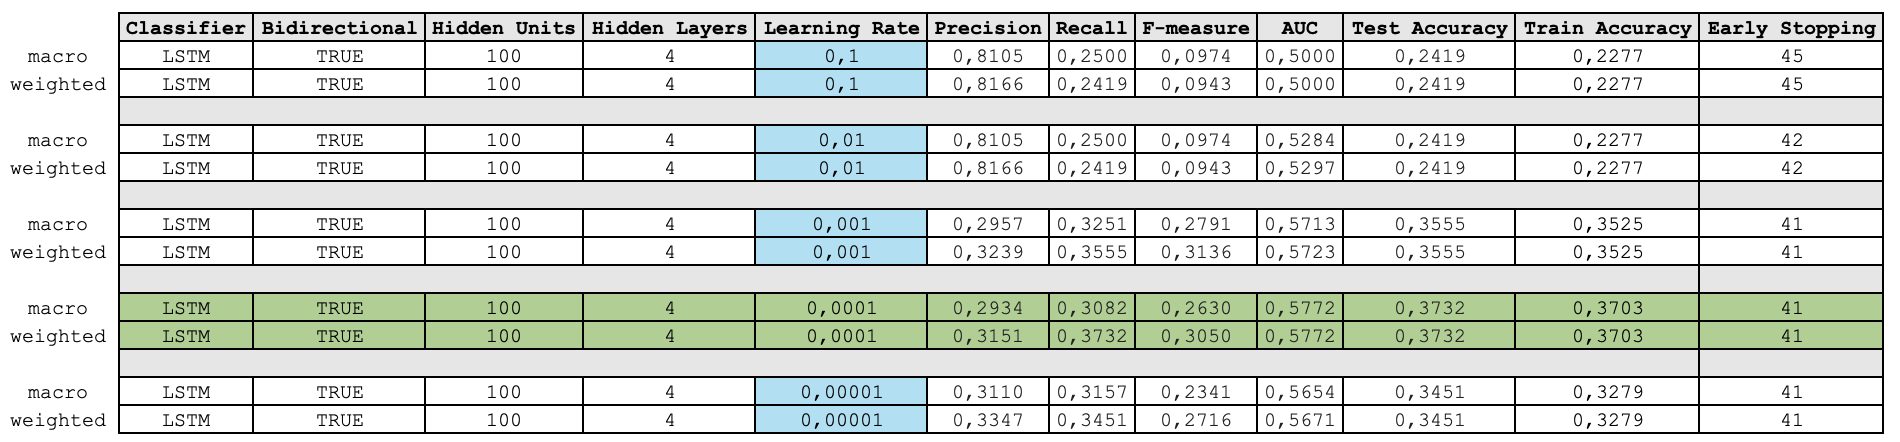
\includegraphics[width=1.2\linewidth]{appendix_tables/engl_lr_table.png}}
\caption{English Level - Learning Rate Experiment Results}
\label{table:engl_lr_table}
\end{table}




\chapter{Age - Experiment Results Tables}\label{appendix:app_age}
\addcontentsline{lot}{chapter}{Age - Experiment Results Tables}
The experiment results for the different variations of model architectures, hidden units, hidden layers and learning rates are provided in this appendix for the age feature. The blue color indicates on which hyperparameter we experimented in each table. The best performance is colored green in all the individual tables.\\

\begin{table}[!ht]
\centerline{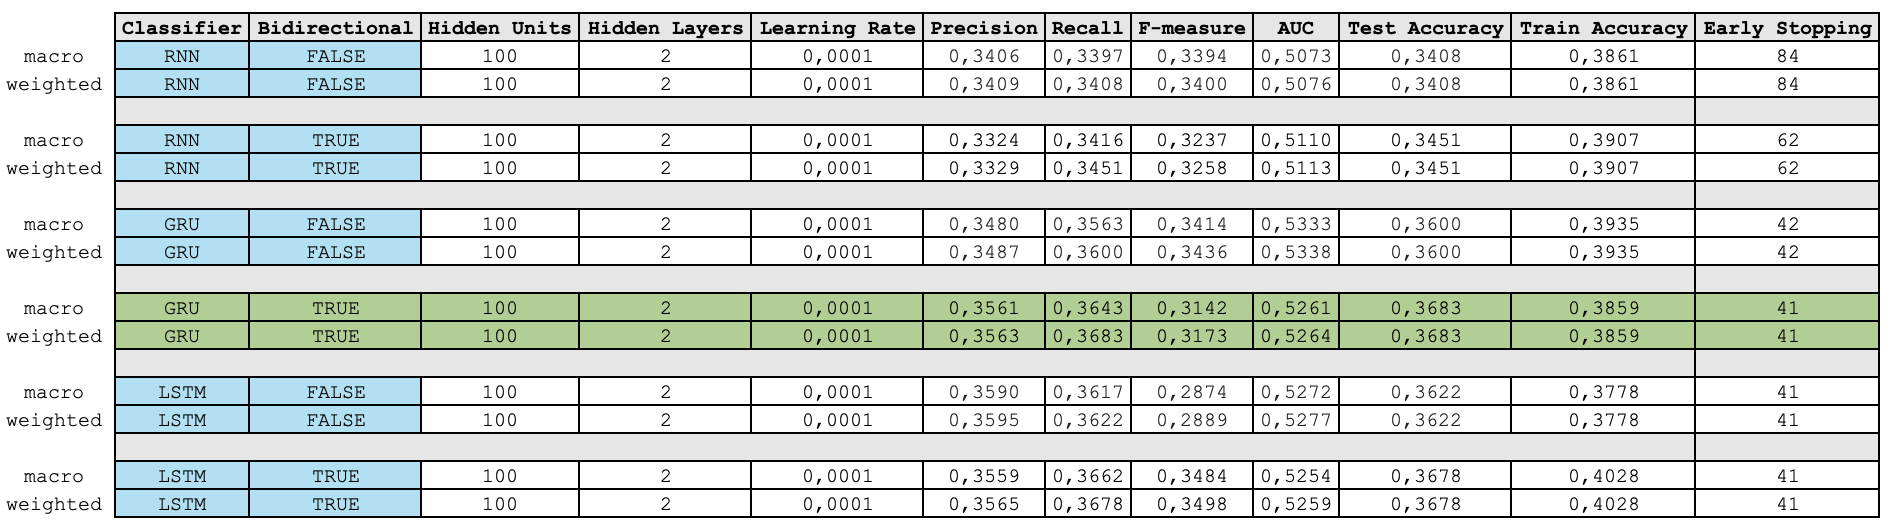
\includegraphics[width=1.2\linewidth]{appendix_tables/age_models_table.png}}
\caption{Age - Models Experiment Results}
\label{table:age_models_table}
\end{table}

\begin{table}[!ht]
\centerline{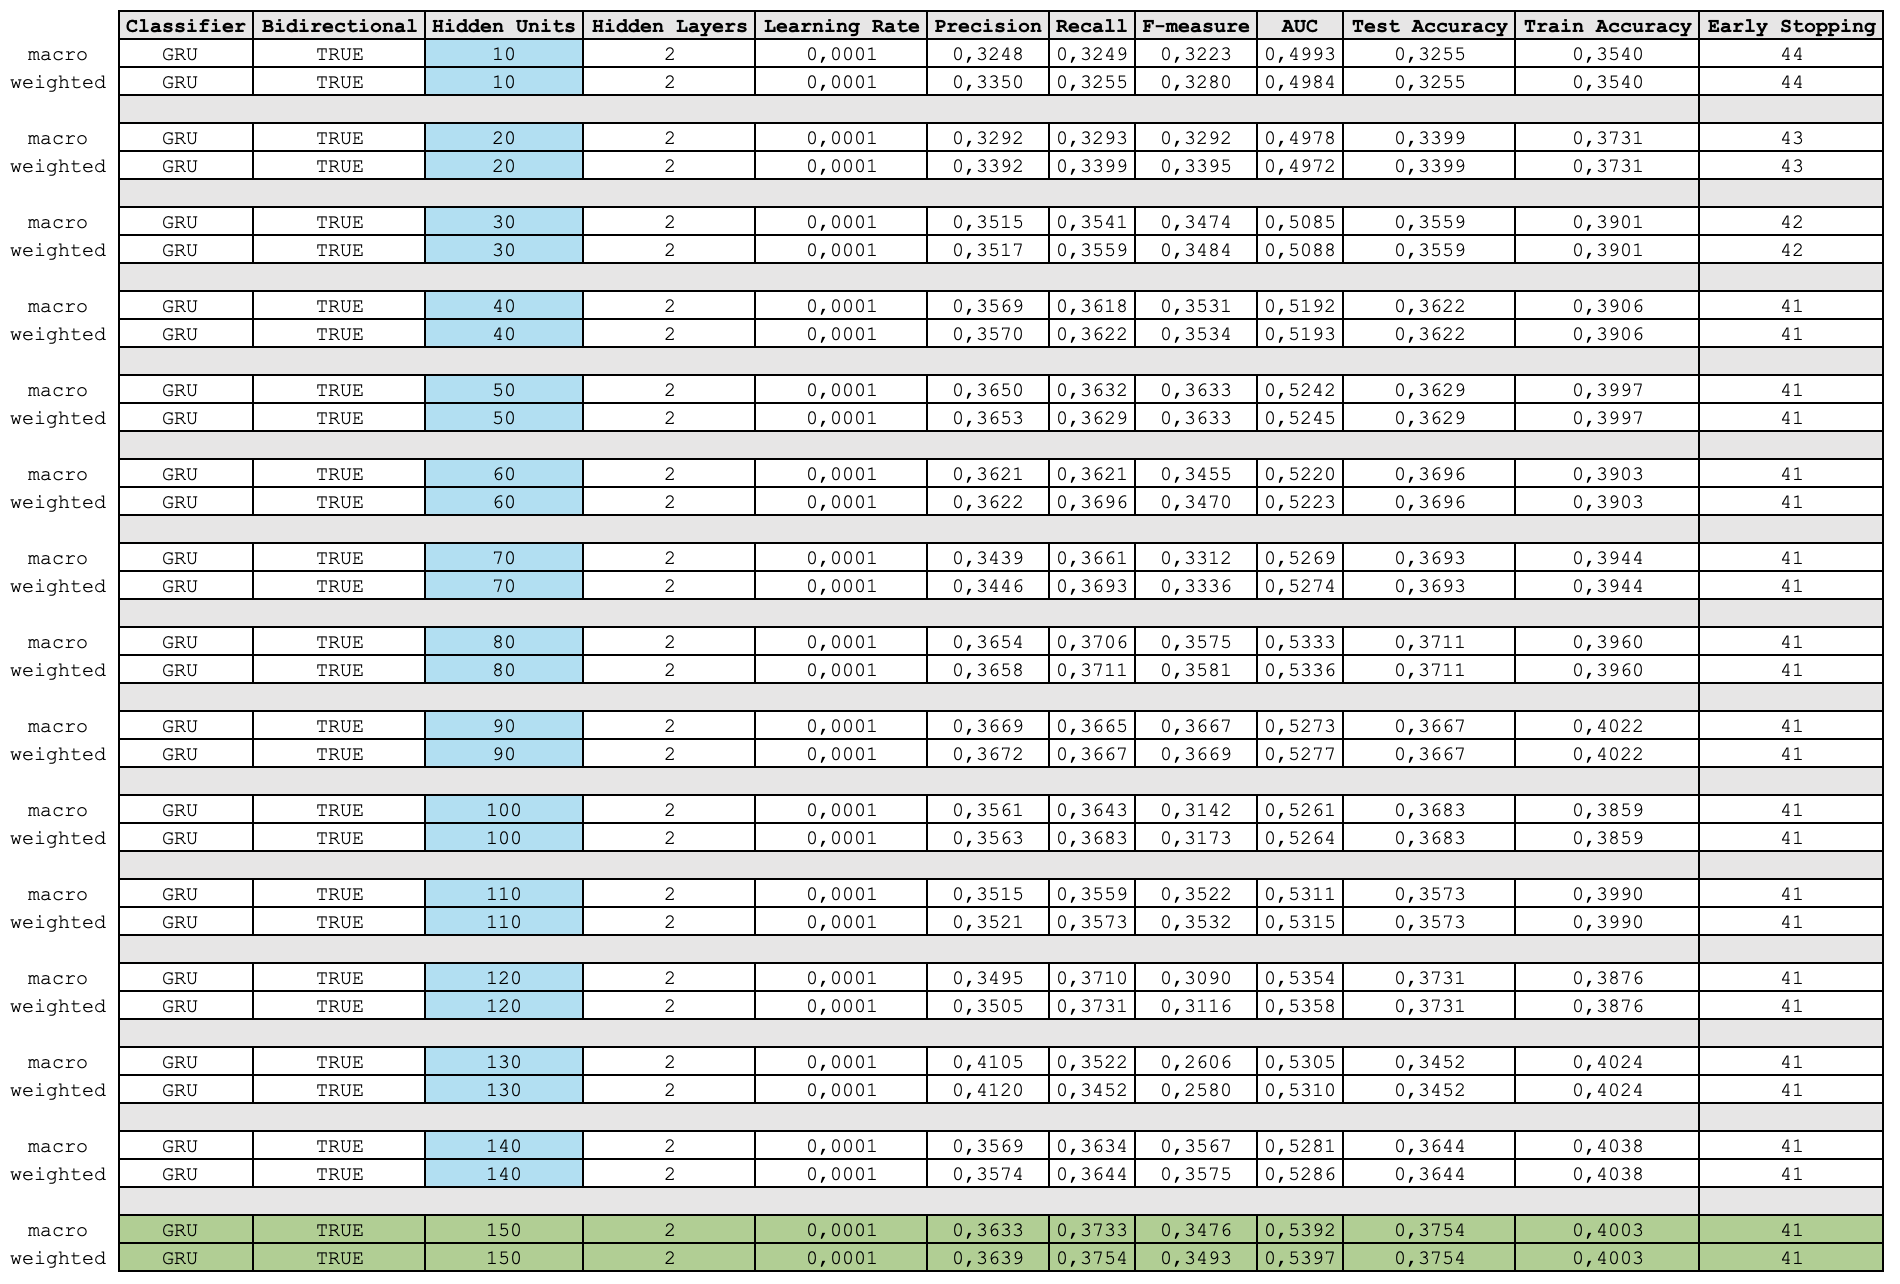
\includegraphics[width=1.2\linewidth]{appendix_tables/age_units_table.png}}
\caption{Age - Hidden Units Experiment Results}
\label{table:age_units_table}
\end{table}

\begin{table}[!ht]
\centerline{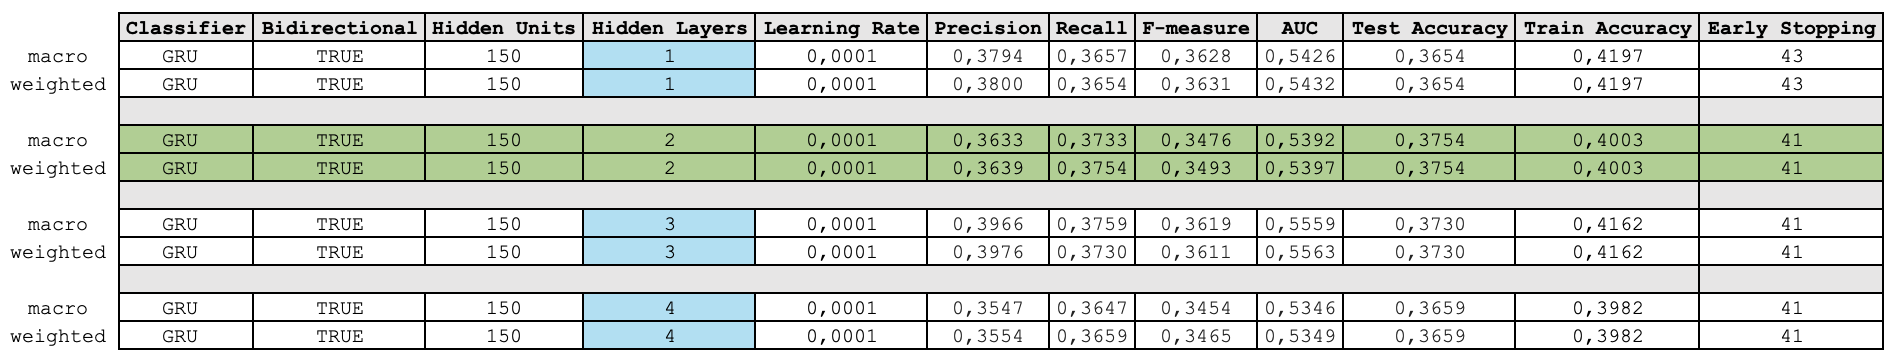
\includegraphics[width=1.2\linewidth]{appendix_tables/age_layers_table.png}}
\caption{Age - Hidden Layers Experiment Results}
\label{table:age_layers_table}
\end{table}

\begin{table}[!ht]
\centerline{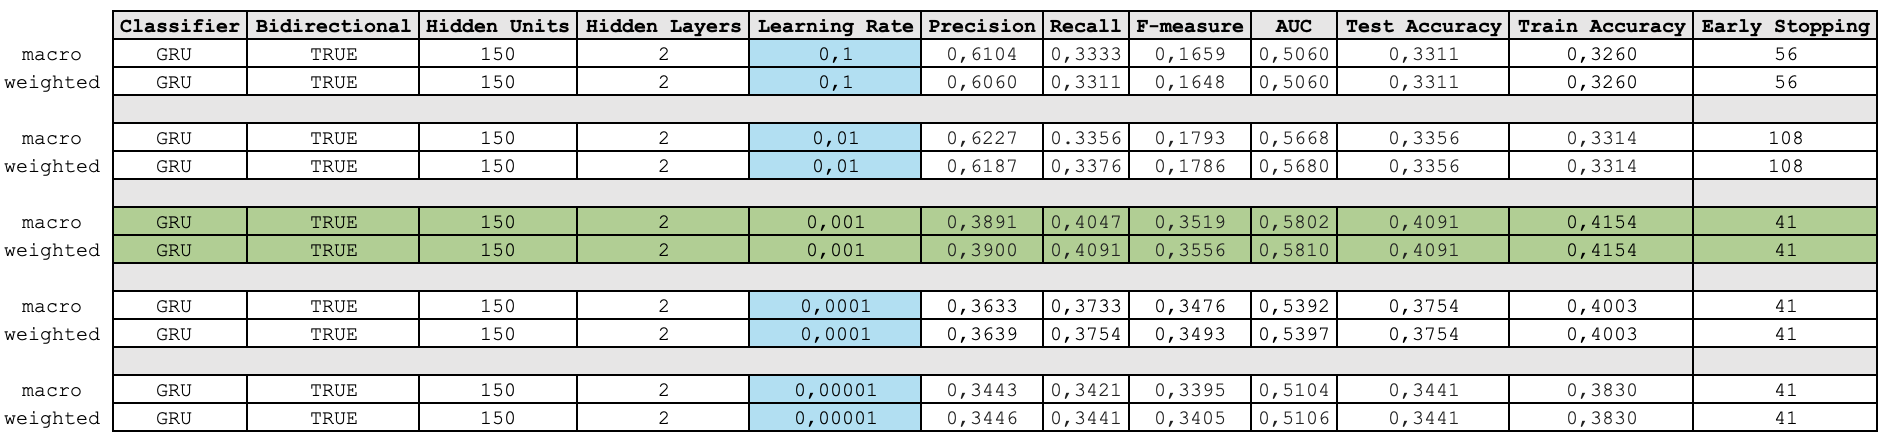
\includegraphics[width=1.2\linewidth]{appendix_tables/age_lr_table.png}}
\caption{Age - Learning Rate Experiment Results}
\label{table:age_lr_table}
\end{table}




\chapter{Nationality - Experiment Results Tables}\label{appendix:app_nat}
\addcontentsline{lot}{chapter}{Nationality - Experiment Results Tables}
The experiment results for the different variations of model architectures, hidden units, hidden layers and learning rates are provided in this appendix for the nationality feature. The blue color indicates on which hyperparameter we experimented in each table. The best performance is colored green in all the individual tables.\\

\begin{table}[!ht]
\centerline{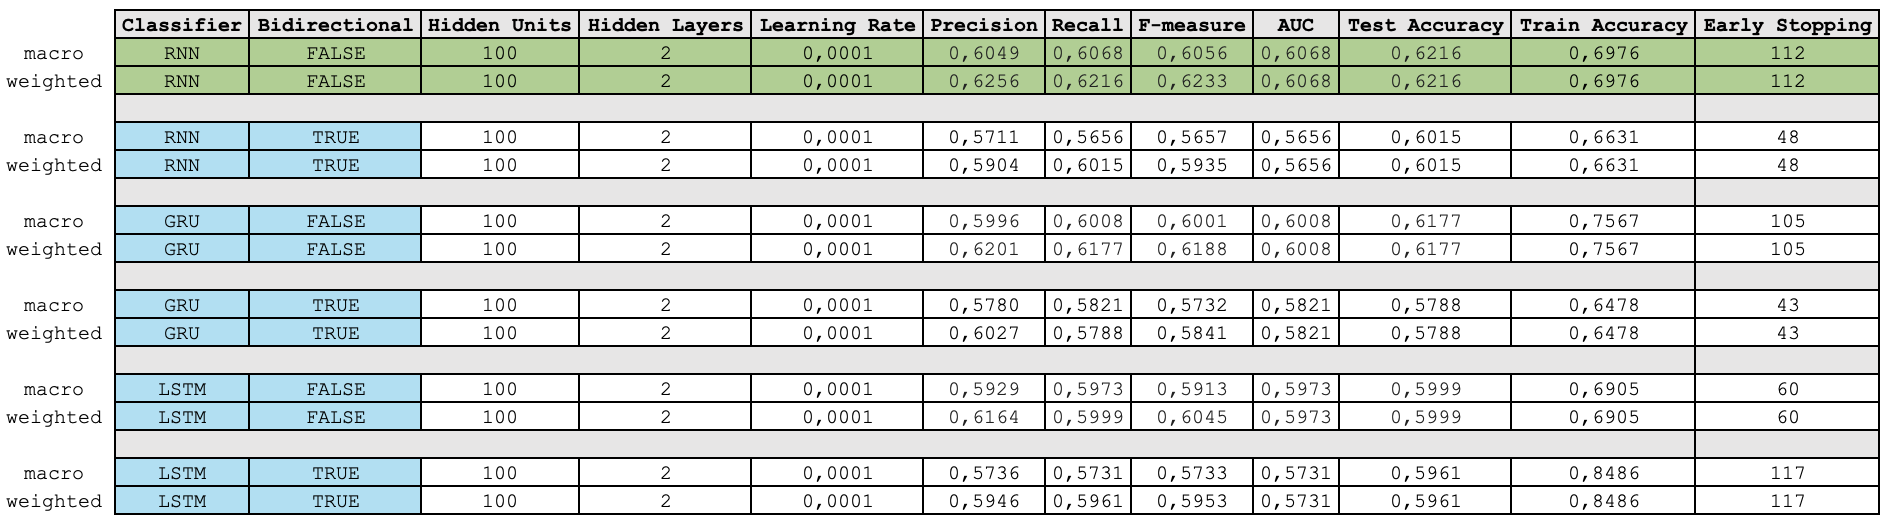
\includegraphics[width=1.2\linewidth]{appendix_tables/nat_models_table.png}}
\caption{Nationality - Models Experiment Results}
\label{table:nat_models_table}
\end{table}

\begin{table}[!ht]
\centerline{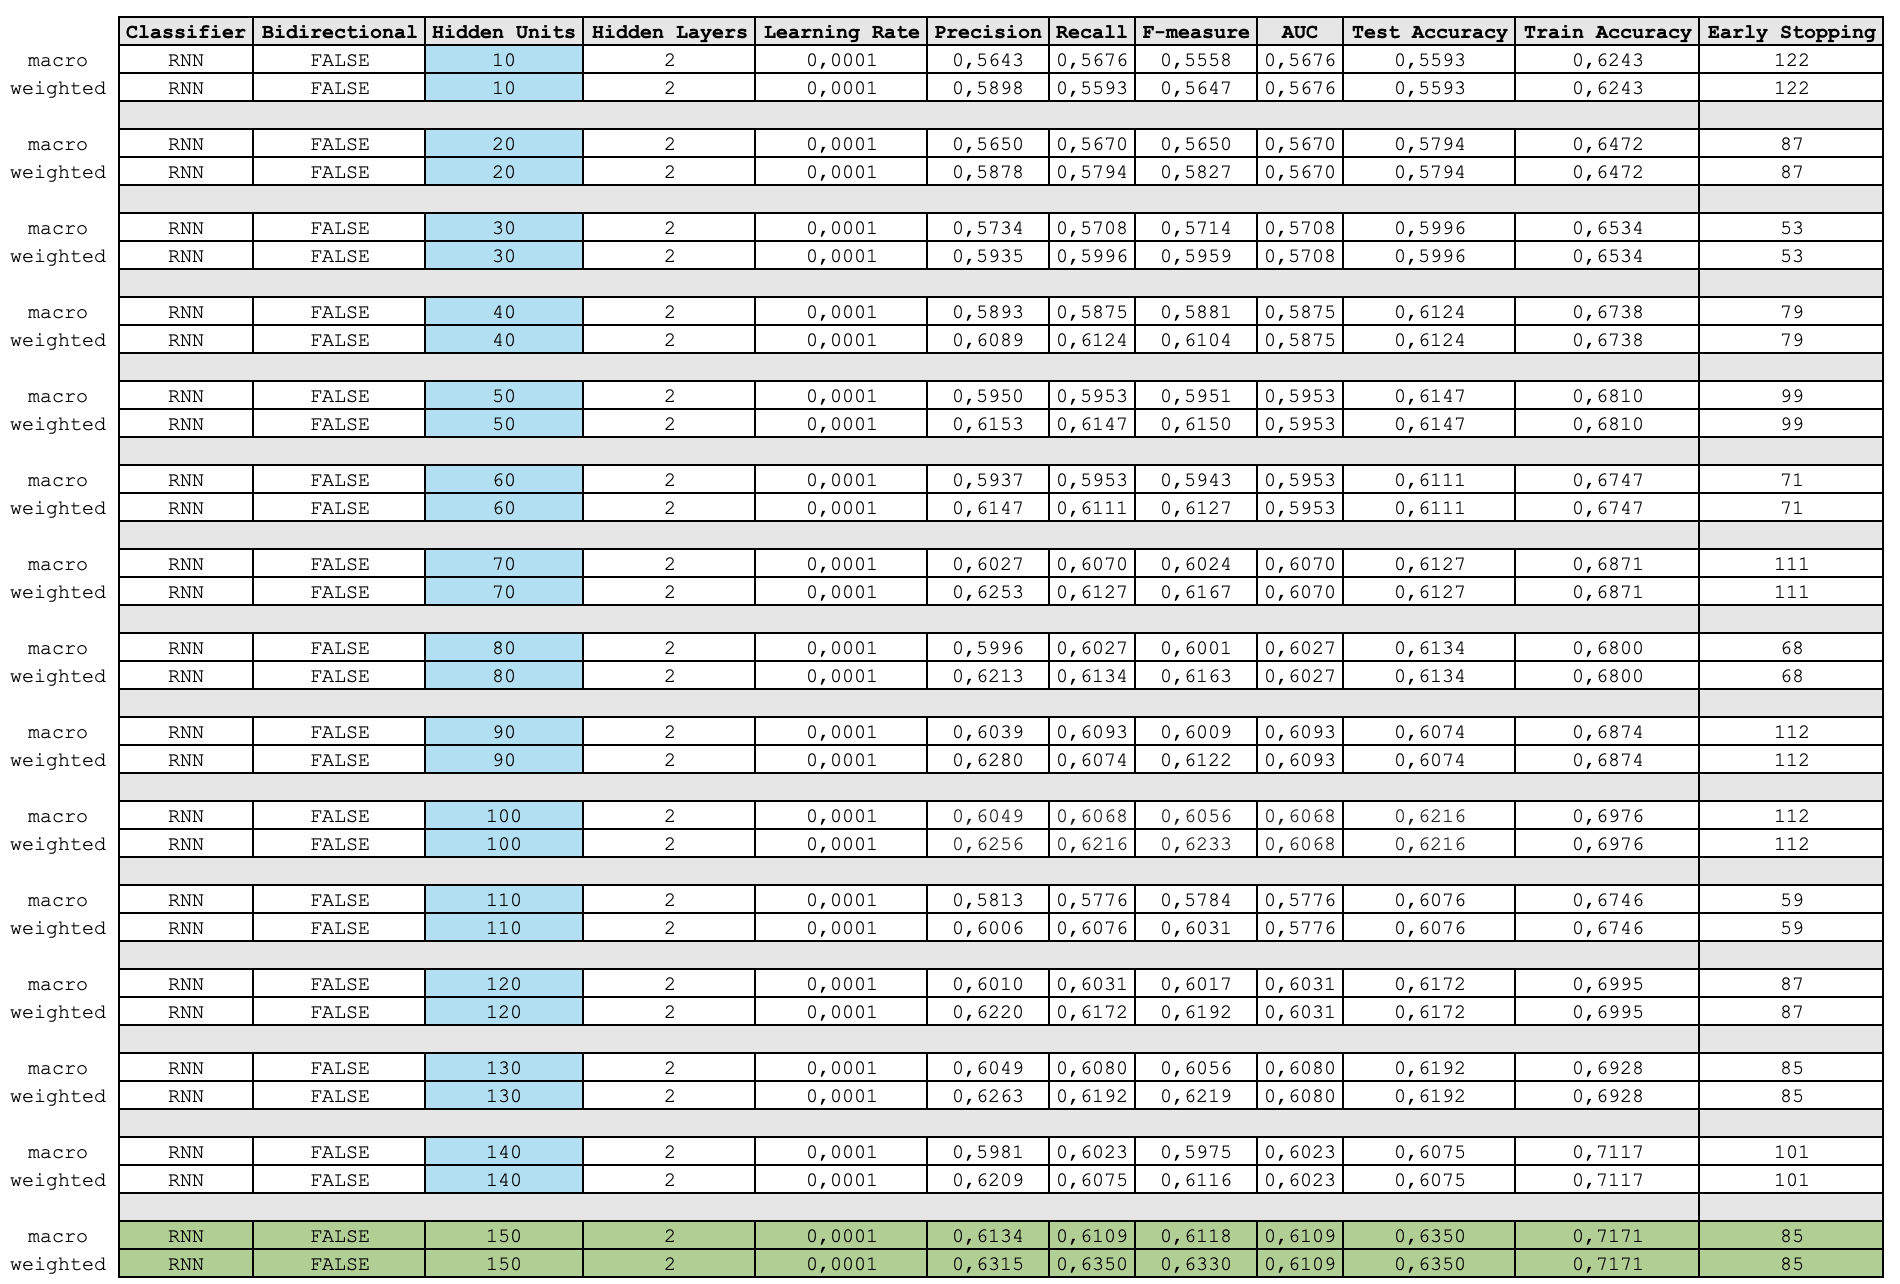
\includegraphics[width=1.2\linewidth]{appendix_tables/nat_units_table.png}}
\caption{Nationality- Hidden Units Experiment Results}
\label{table:nat_units_table}
\end{table}

\begin{table}[!ht]
\centerline{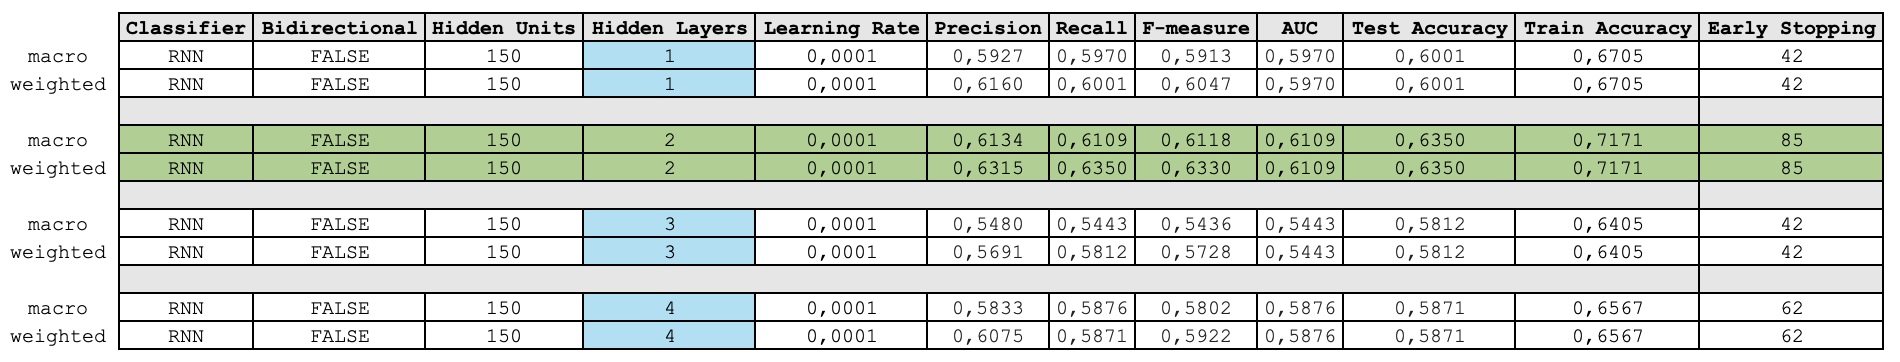
\includegraphics[width=1.2\linewidth]{appendix_tables/nat_layers_table.png}}
\caption{Nationality - Hidden Layers Experiment Results}
\label{table:nat_layers_table}
\end{table}

\begin{table}[!ht]
\centerline{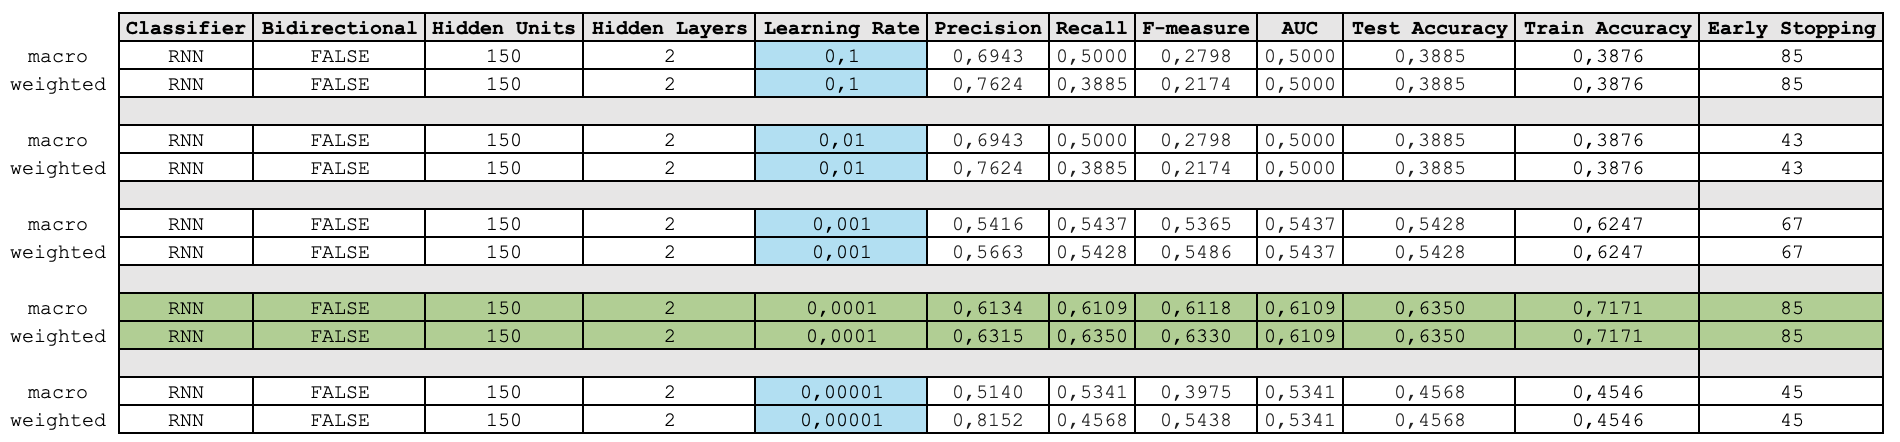
\includegraphics[width=1.2\linewidth]{appendix_tables/nat_lr_table.png}}
\caption{Nationality - Learning Rate Experiment Results}
\label{table:nat_lr_table}
\end{table}




\chapter{Gender - Experiment Results Tables}\label{appendix:app_gender}
\addcontentsline{lot}{chapter}{Gender - Experiment Results Tables}
The experiment results for the different variations of model architectures, hidden units, hidden layers and learning rates are provided in this appendix for the gender feature. The blue color indicates on which hyperparameter we experimented in each table. The best performance is colored green in all the individual tables.\\

\begin{table}[!ht]
\centerline{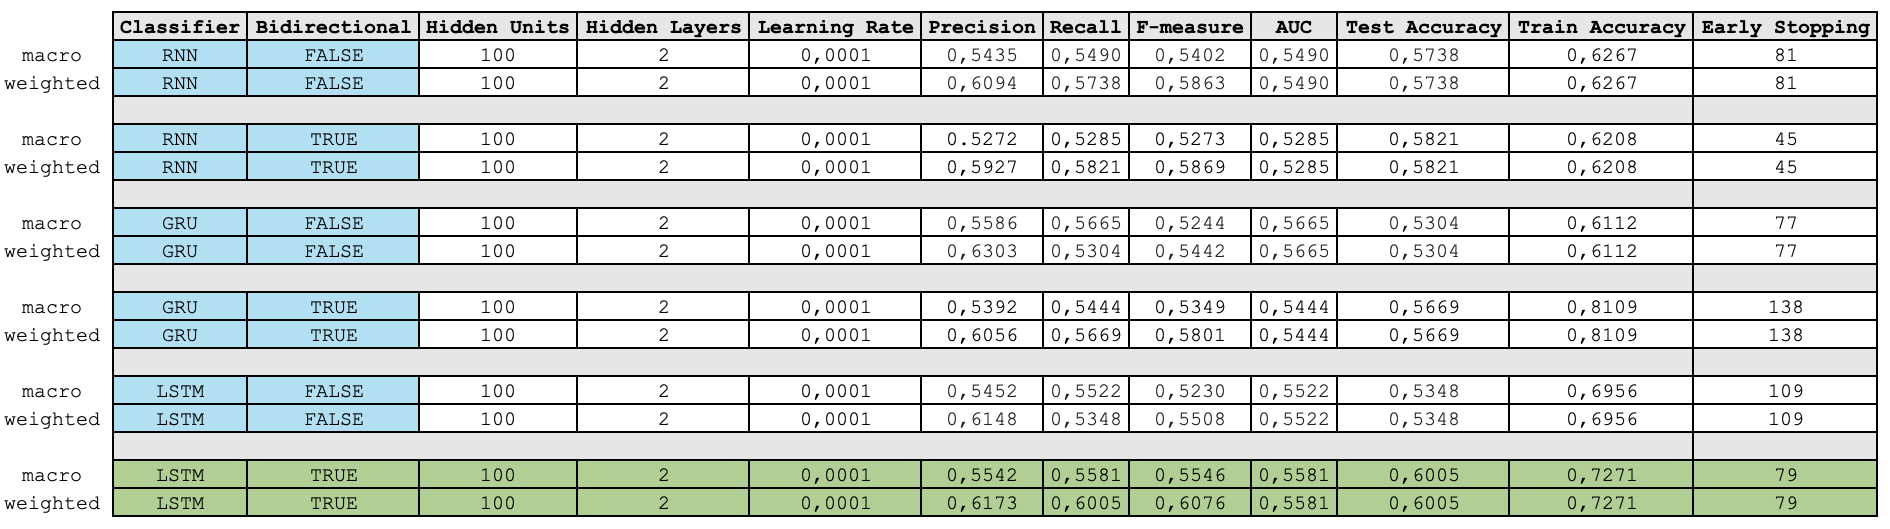
\includegraphics[width=1.2\linewidth]{appendix_tables/gender_models_table.png}}
\caption{Gender - Models Experiment Results}
\label{table:gender_models_table}
\end{table}

\begin{table}[!ht]
\centerline{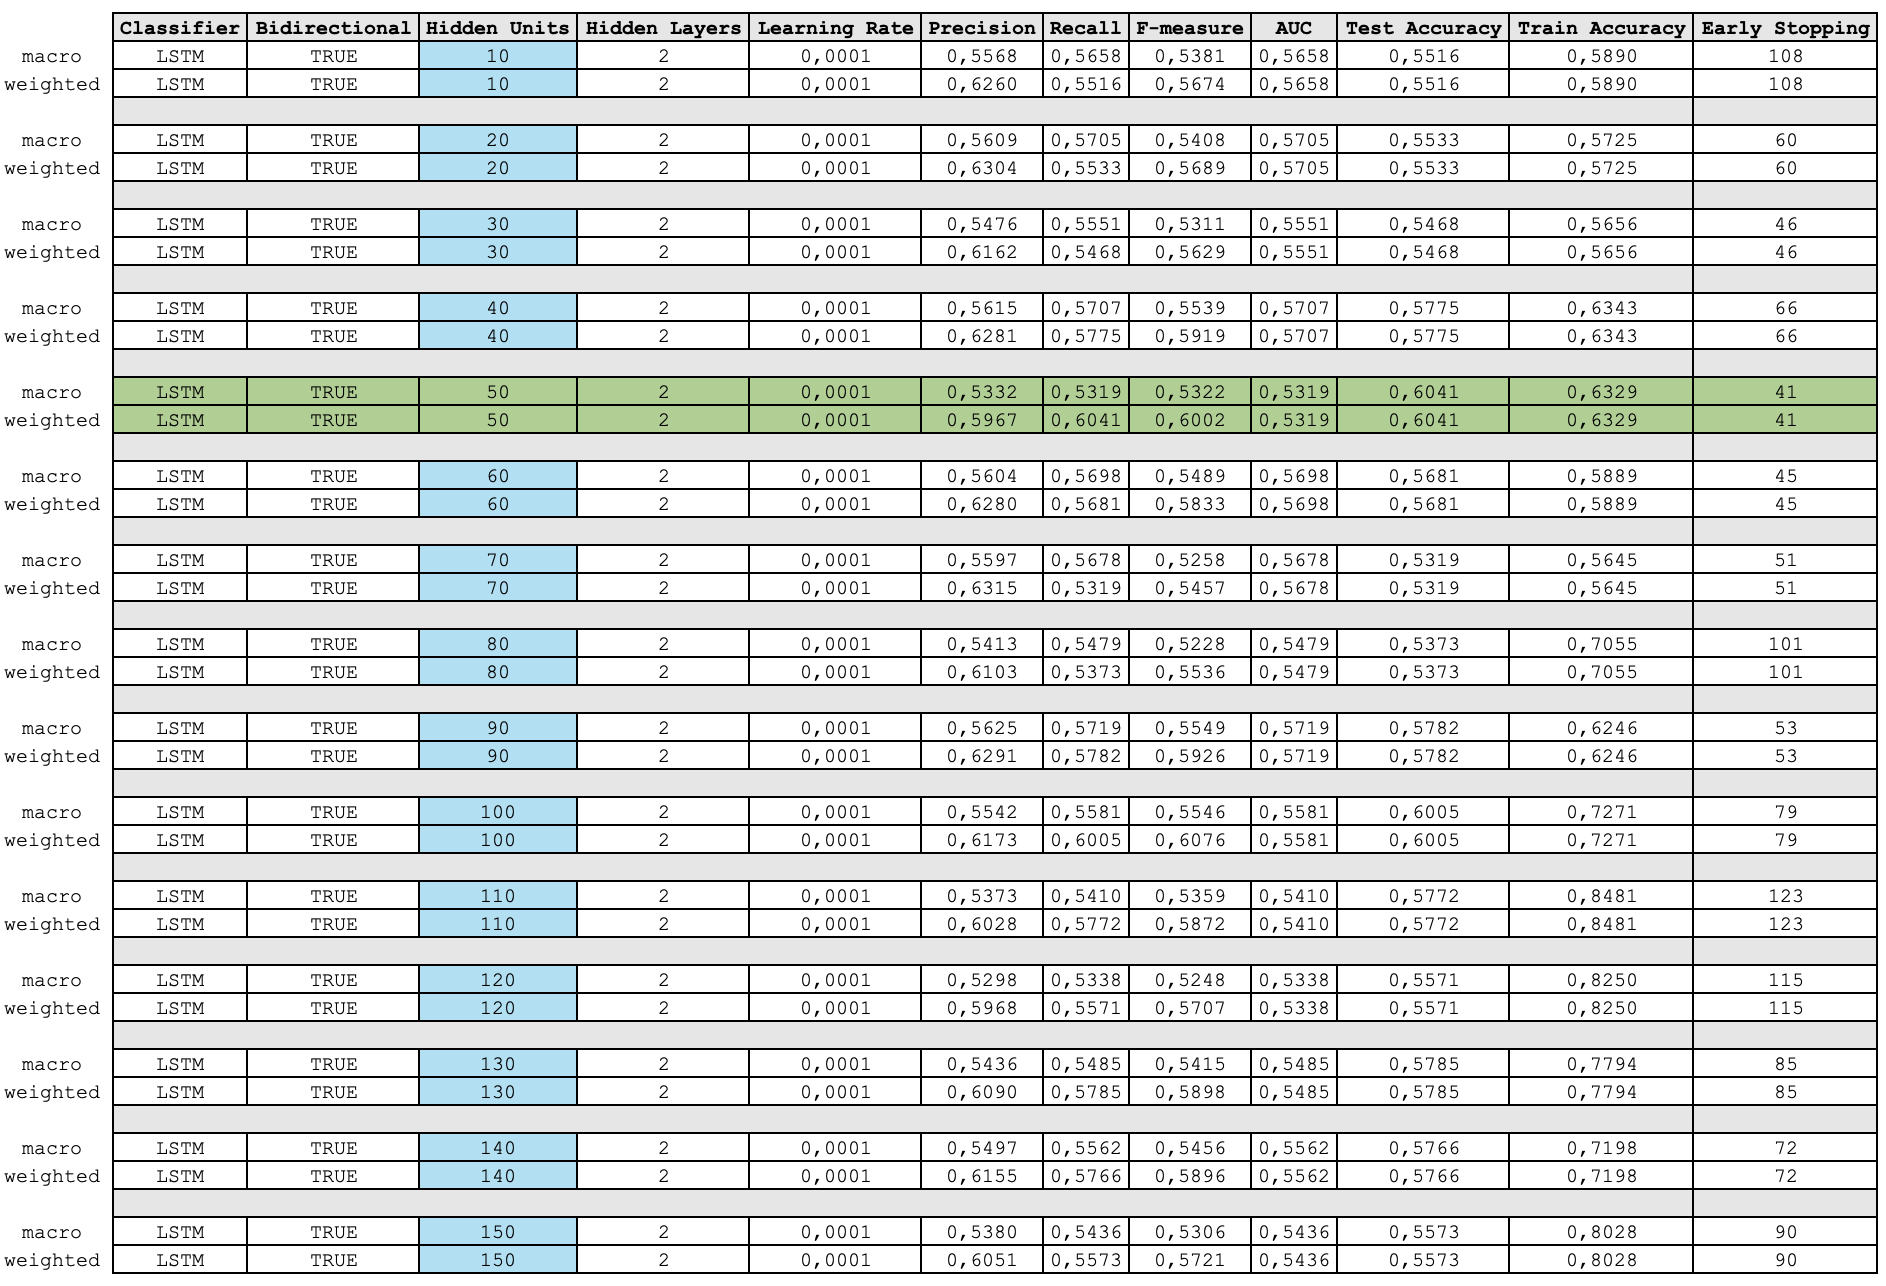
\includegraphics[width=1.2\linewidth]{appendix_tables/gender_units_table.png}}
\caption{Gender - Hidden Units Experiment Results}
\label{table:gender_units_table}
\end{table}

\begin{table}[!ht]
\centerline{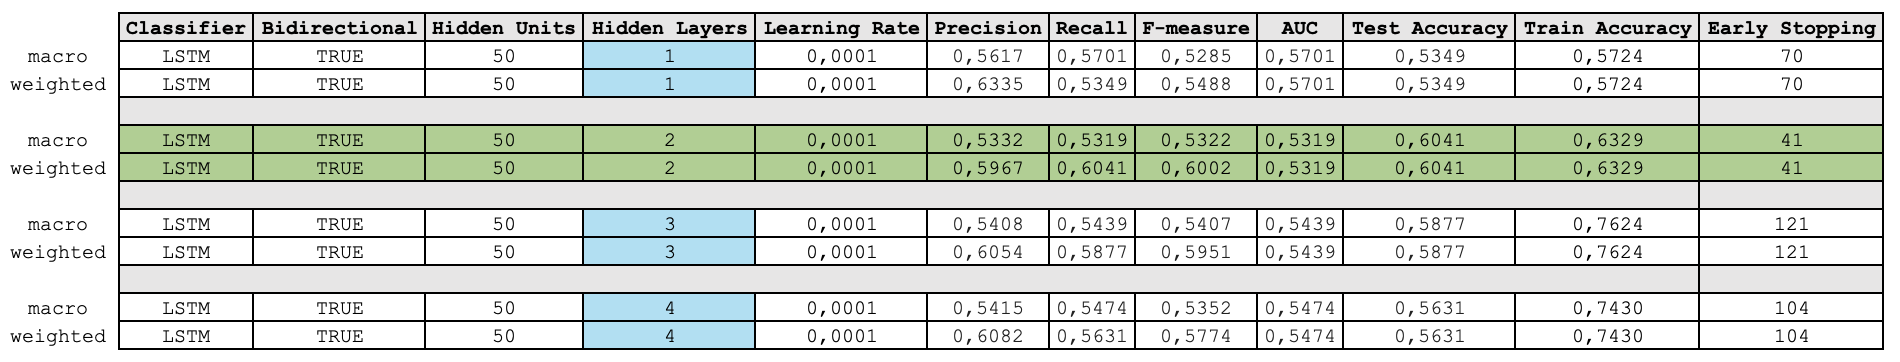
\includegraphics[width=1.2\linewidth]{appendix_tables/gender_layers_table.png}}
\caption{Gender - Hidden Layers Experiment Results}
\label{table:gender_layers_table}
\end{table}

\begin{table}[!ht]
\centerline{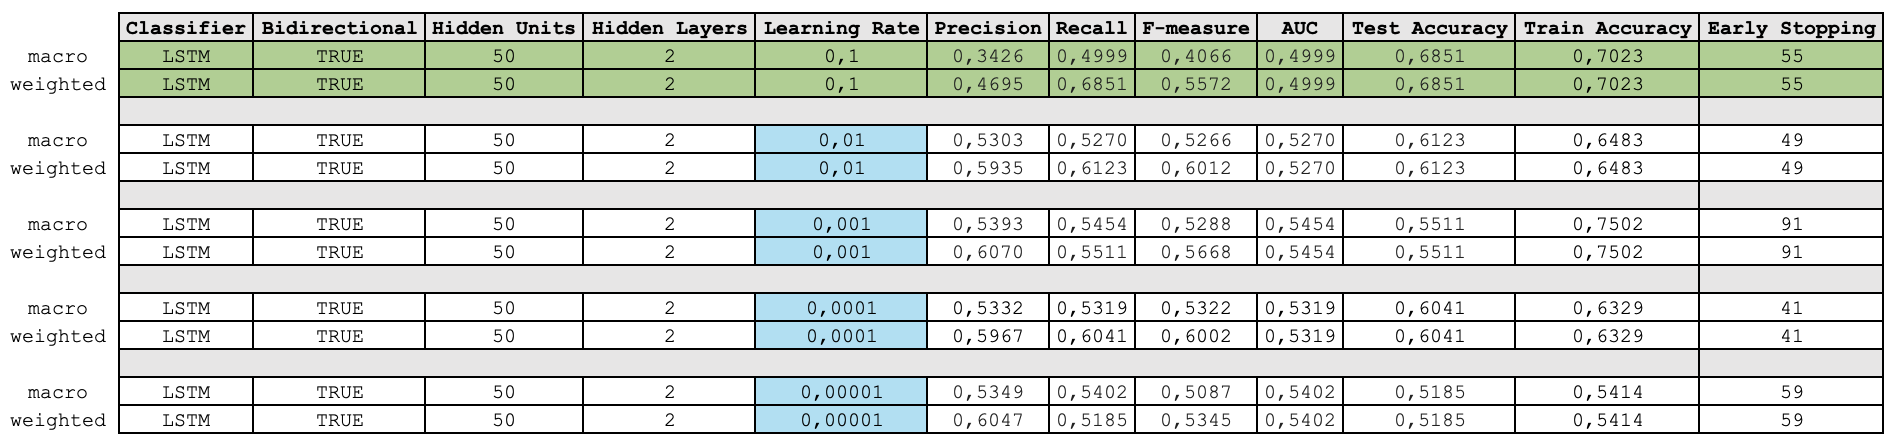
\includegraphics[width=1.2\linewidth]{appendix_tables/gender_lr_table.png}}
\caption{Gender - Learning Rate Experiment Results}
\label{table:gender_lr_table}
\end{table}




\chapter{Dominant Hand - Experiment Results Tables}\label{appendix:app_dom}
\addcontentsline{lot}{chapter}{Dominant Hand - Experiment Results Tables}
The experiment results for the different variations of model architectures, hidden units, hidden layers and learning rates are provided in this appendix for the dominant hand feature. The blue color indicates on which hyperparameter we experimented in each table. The best performance is colored green in all the individual tables.\\

\begin{table}[!ht]
\centerline{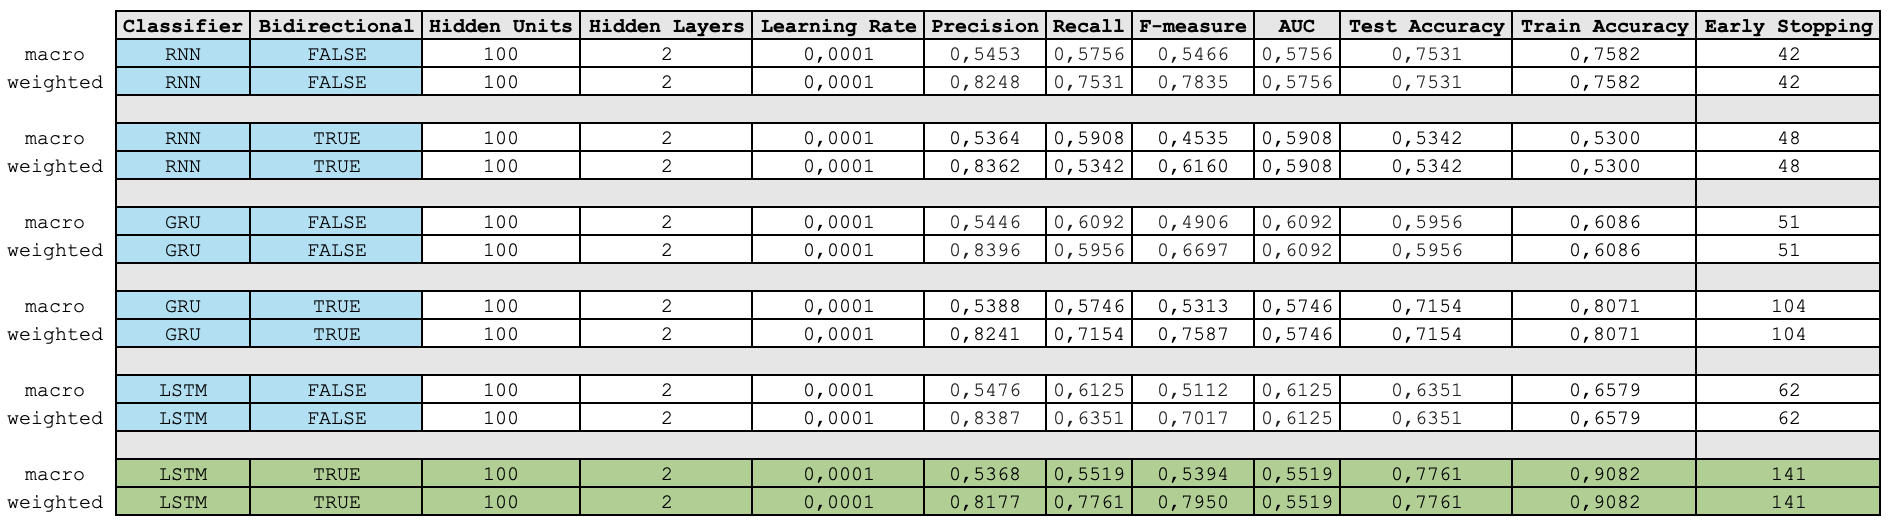
\includegraphics[width=1.2\linewidth]{appendix_tables/dom_models_table.png}}
\caption{Dominant Hand - Models Experiment Results}
\label{table:dom_models_table}
\end{table}

\begin{table}[!ht]
\centerline{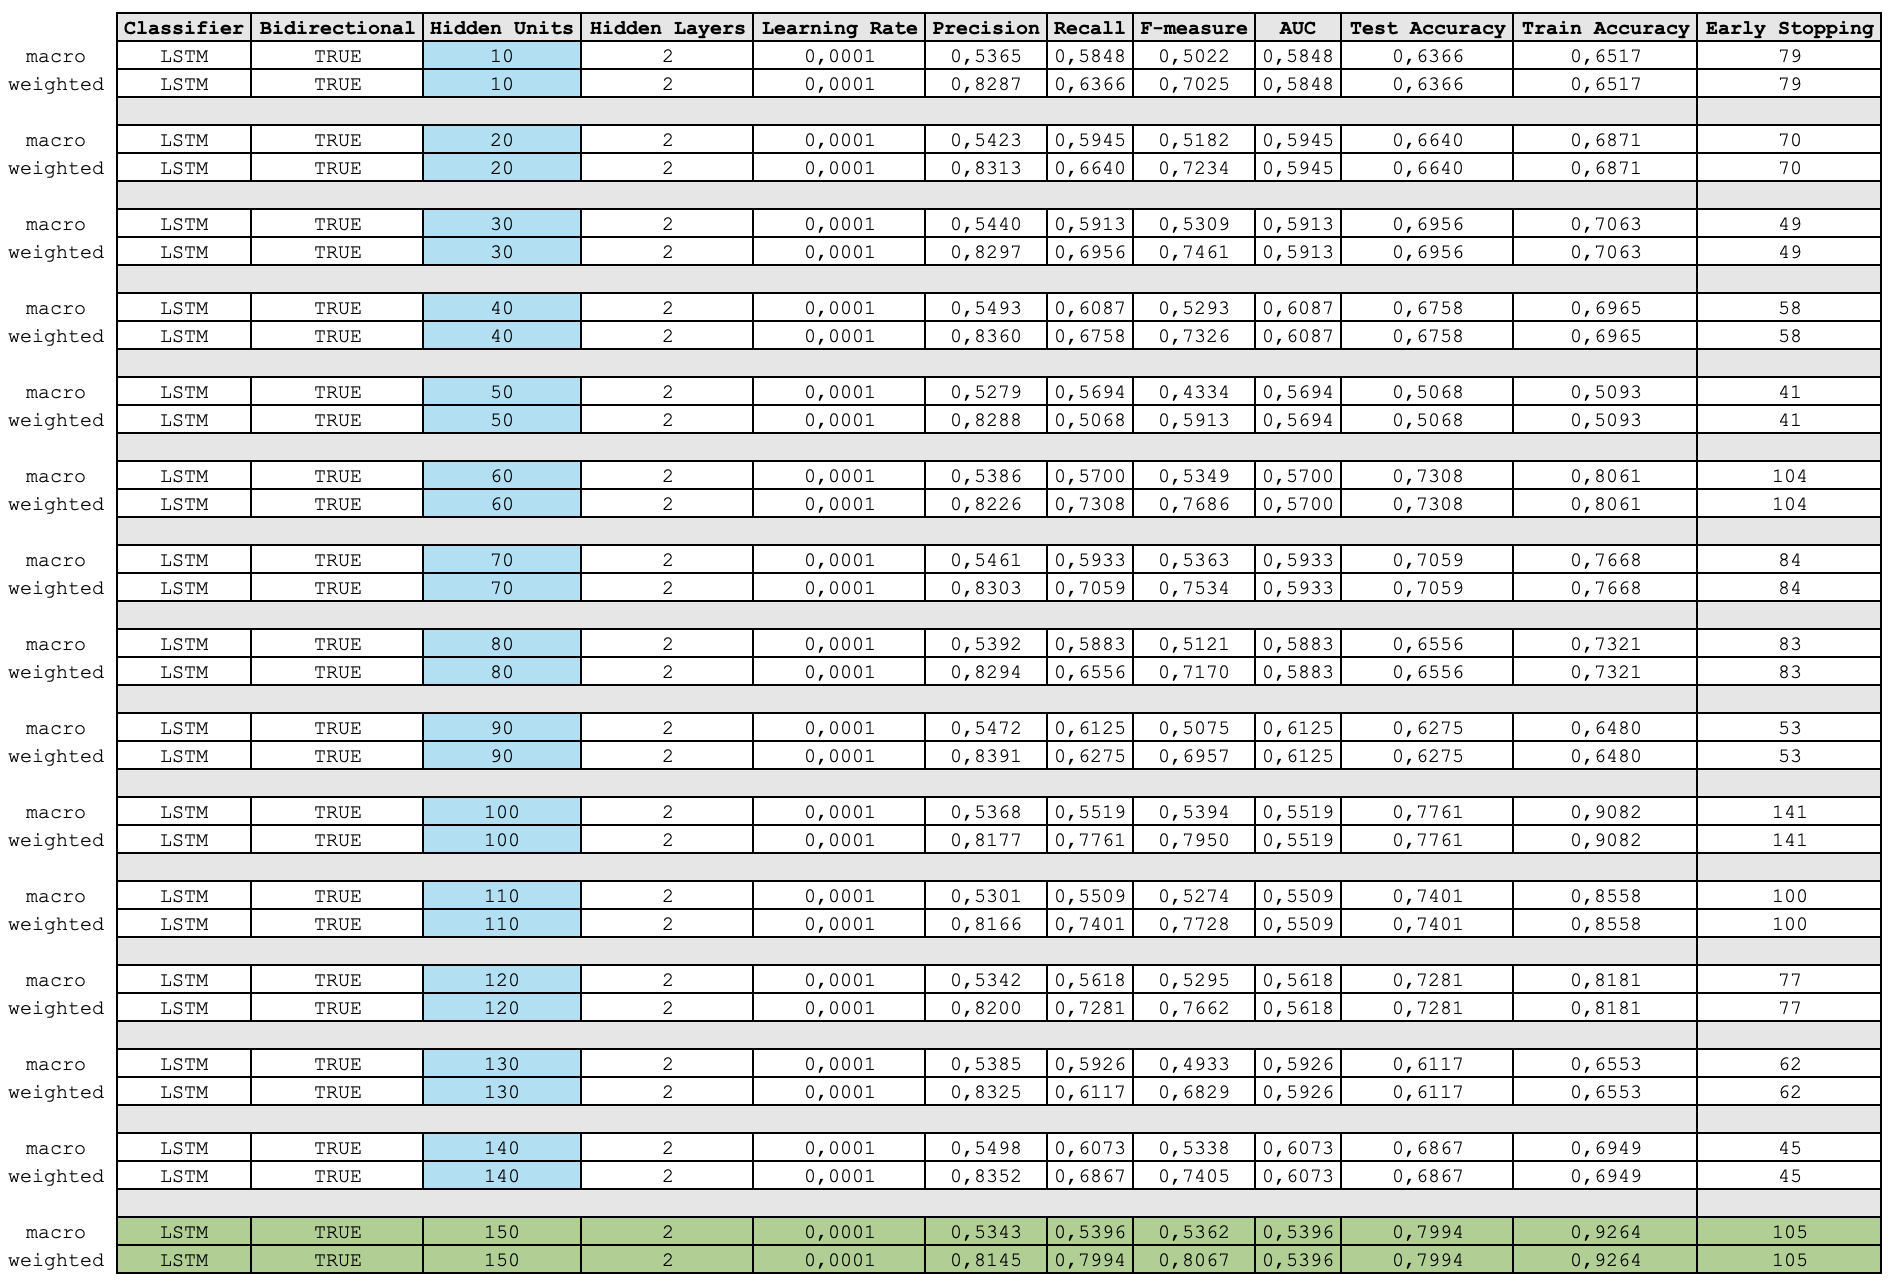
\includegraphics[width=1.2\linewidth]{appendix_tables/dom_units_table.png}}
\caption{Dominant Hand - Hidden Units Experiment Results}
\label{table:dom_units_table}
\end{table}

\begin{table}[!ht]
\centerline{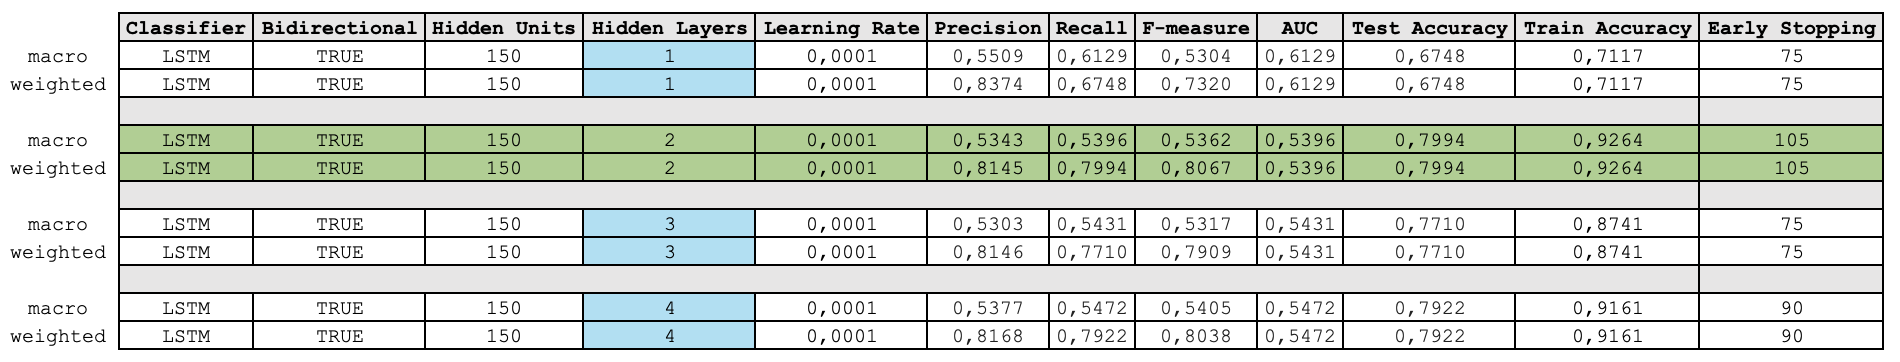
\includegraphics[width=1.2\linewidth]{appendix_tables/dom_layers_table.png}}
\caption{Dominant Hand - Hidden Layers Experiment Results}
\label{table:dom_layers_table}
\end{table}

\begin{table}[!ht]
\centerline{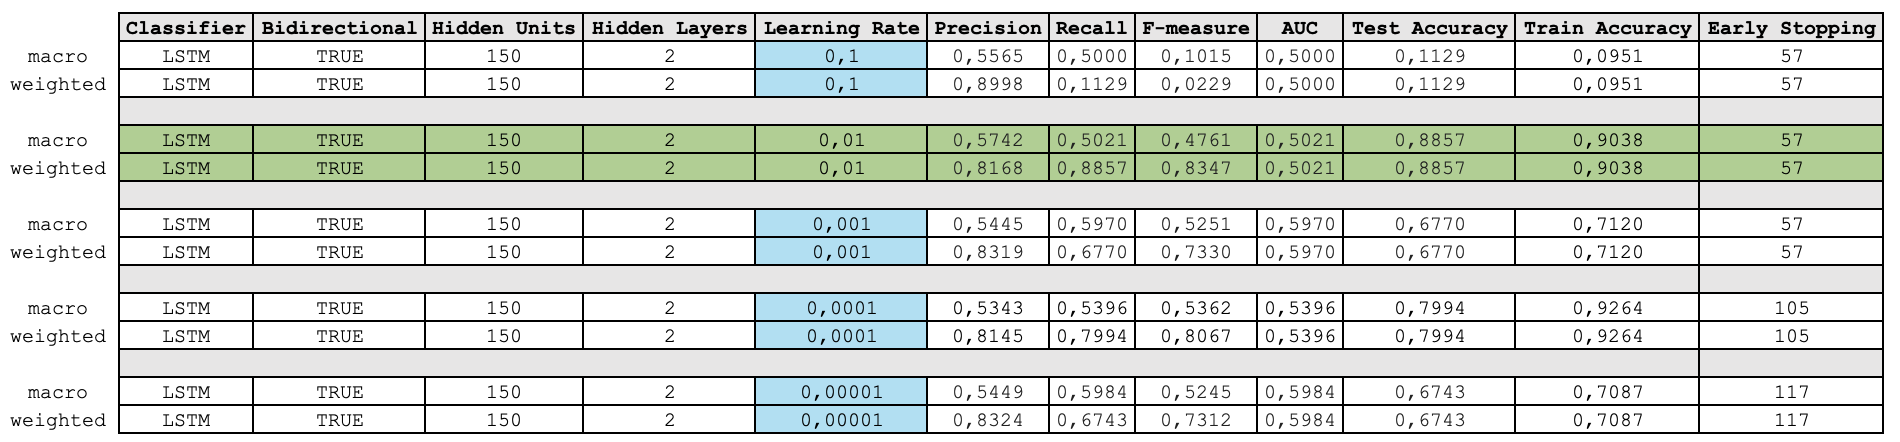
\includegraphics[width=1.2\linewidth]{appendix_tables/dom_lr_table.png}}
\caption{Dominant Hand - Learning Rate Experiment Results}
\label{table:dom_lr_table}
\end{table}




\chapter{Swipe Hand - Experiment Results Tables}\label{appendix:app_hand}
\addcontentsline{lot}{chapter}{Swipe Hand - Experiment Results Tables}
The experiment results for the different variations of model architectures, hidden units, hidden layers and learning rates are provided in this appendix for the swiping hand feature. The blue color indicates on which hyperparameter we experimented in each table. The best performance is colored green in all the individual tables.\\

\begin{table}[!ht]
\centerline{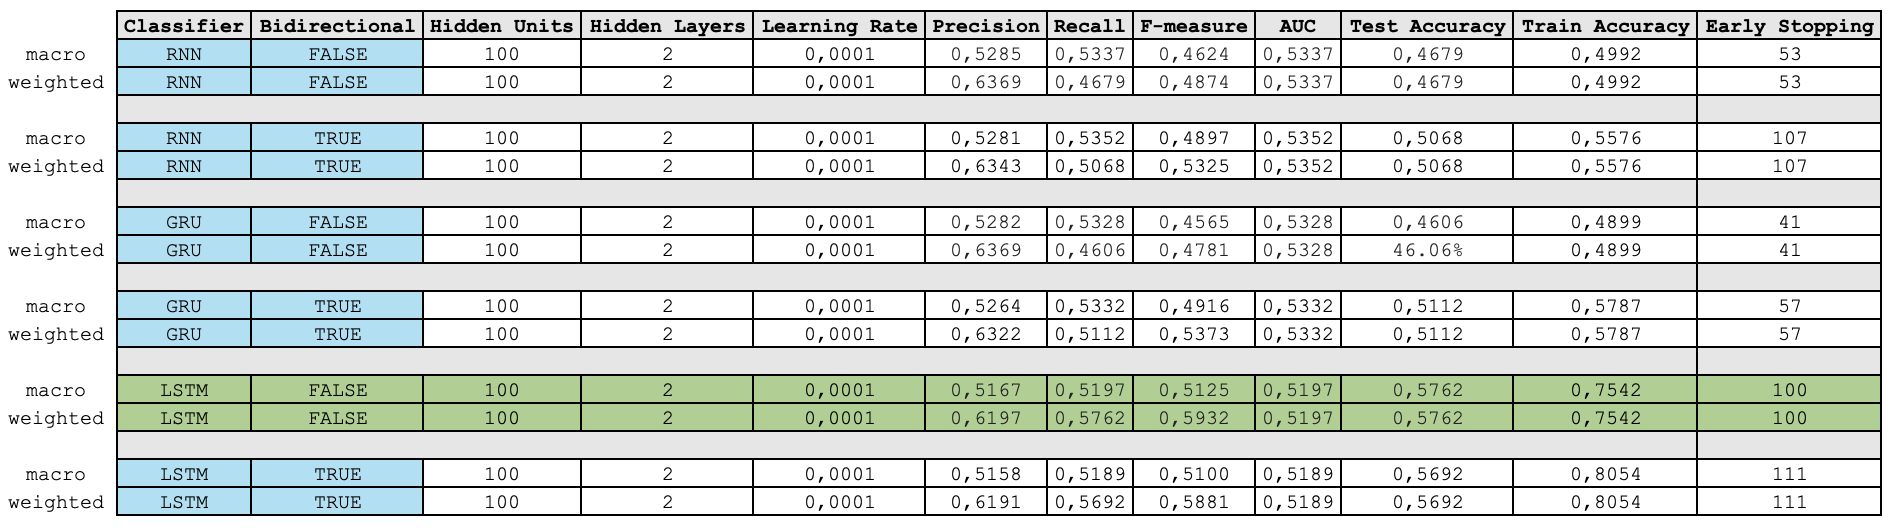
\includegraphics[width=1.2\linewidth]{appendix_tables/hand_models_table.png}}
\caption{Swipe Hand - Models Experiment Results}
\label{table:hand_models_table}
\end{table}

\begin{table}[!ht]
\centerline{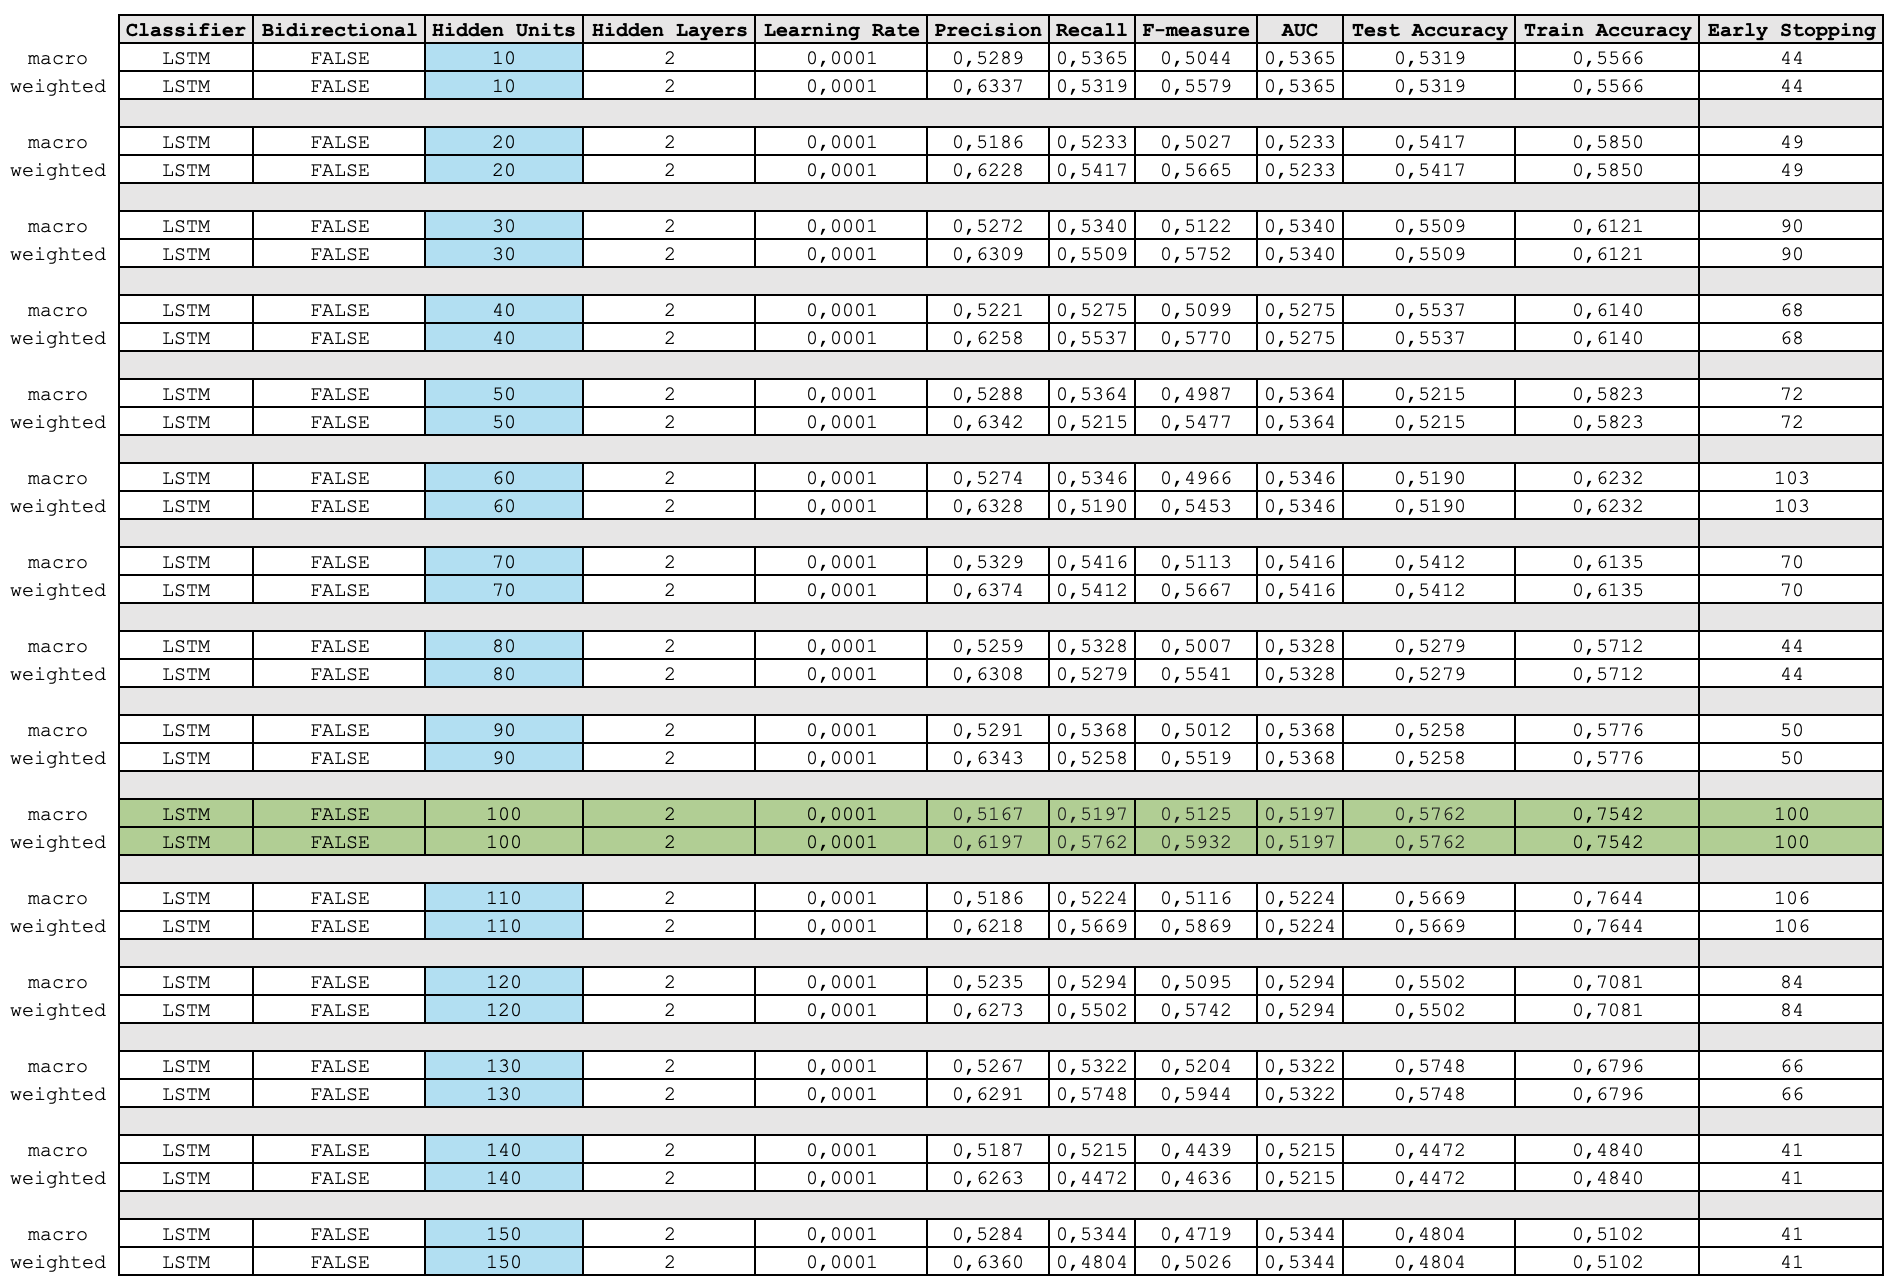
\includegraphics[width=1.2\linewidth]{appendix_tables/hand_units_table.png}}
\caption{Swipe Hand - Hidden Units Experiment Results}
\label{table:hand_units_table}
\end{table}

\begin{table}[!ht]
\centerline{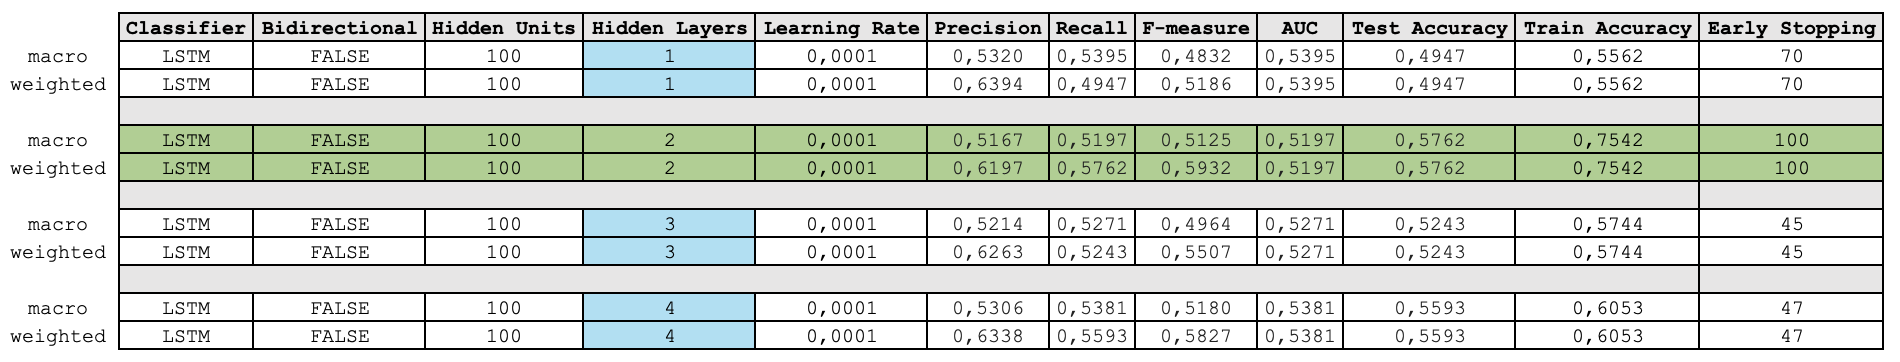
\includegraphics[width=1.2\linewidth]{appendix_tables/hand_layers_table.png}}
\caption{Swipe Hand - Hidden Layers Experiment Results}
\label{table:hand_layers_table}
\end{table}

\begin{table}[!ht]
\centerline{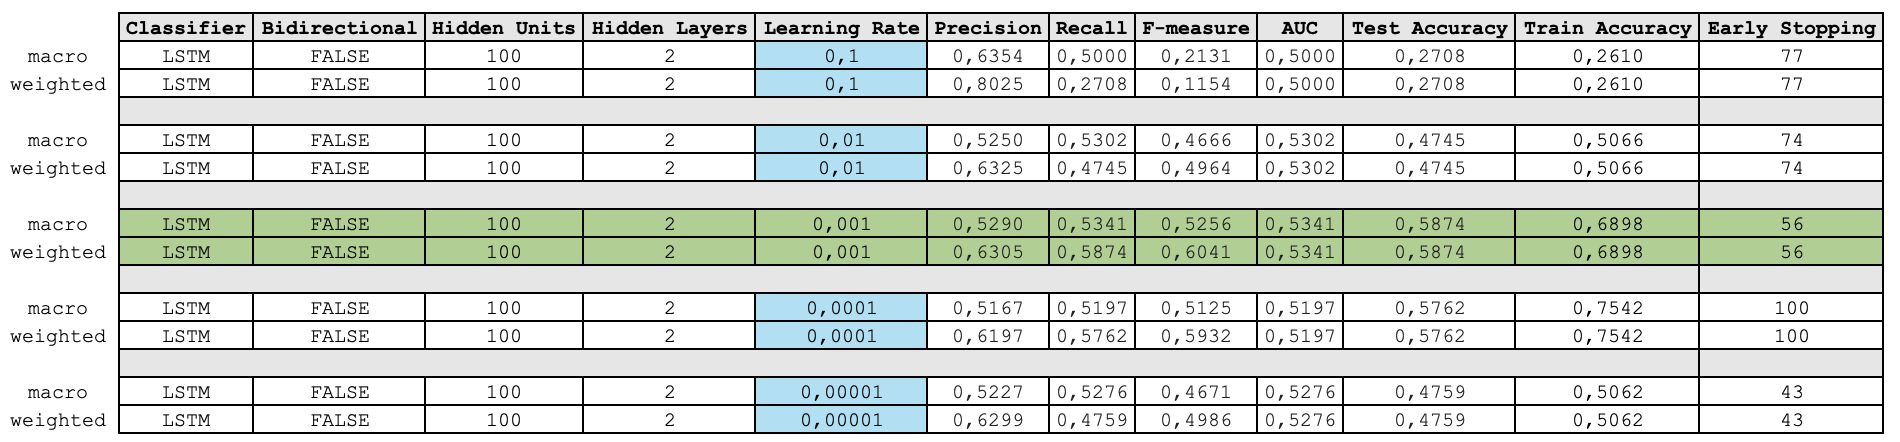
\includegraphics[width=1.2\linewidth]{appendix_tables/hand_lr_table.png}}
\caption{Swipe Hand - Learning Rate Experiment Results}
\label{table:hand_lr_table}
\end{table}




\chapter{Swipe Finger - Experiment Results Tables}\label{appendix:app_finger}
\addcontentsline{lot}{chapter}{Swipe Finger - Experiment Results Tables}
The experiment results for the different variations of model architectures, hidden units, hidden layers and learning rates are provided in this appendix for the swiping finger feature. The blue color indicates on which hyperparameter we experimented in each table. The best performance is colored green in all the individual tables.\\

\begin{table}[!ht]
\centerline{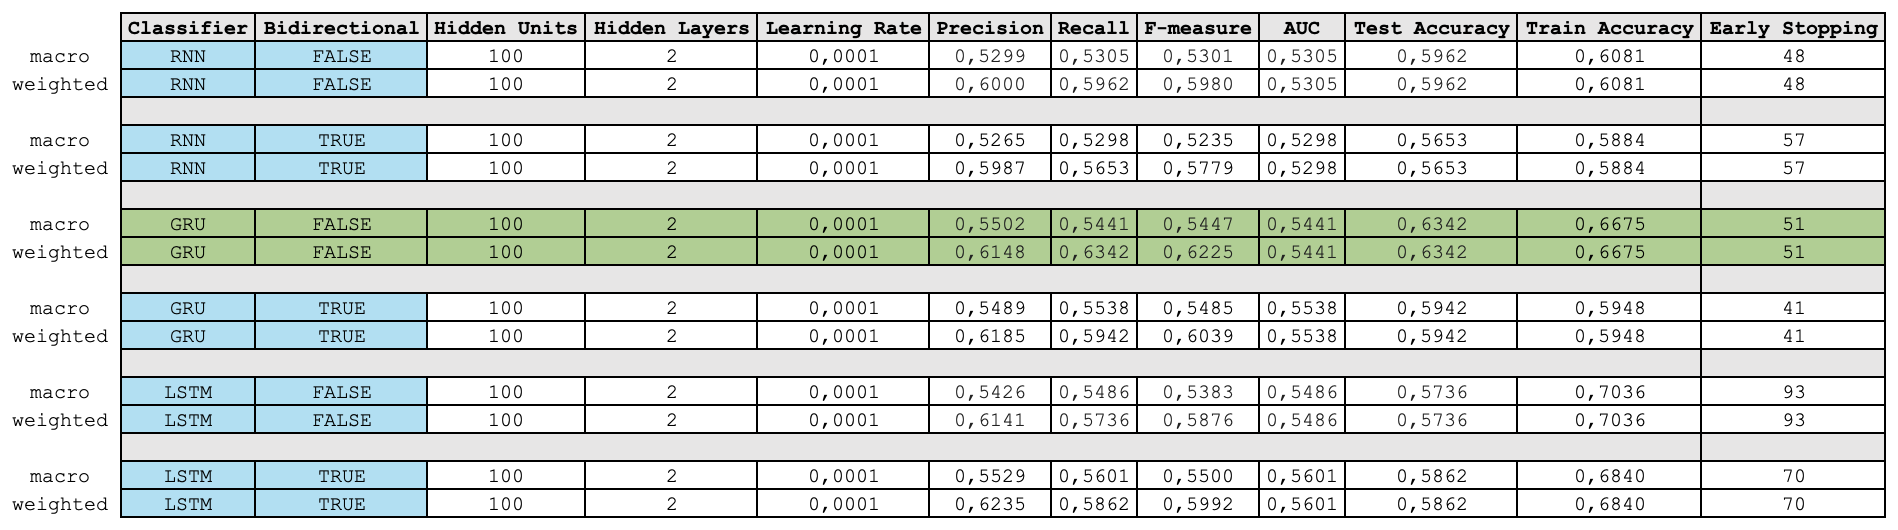
\includegraphics[width=1.2\linewidth]{appendix_tables/finger_models_table.png}}
\caption{Swipe Finger - Models Experiment Results}
\label{table:finger_models_table}
\end{table}

\begin{table}[!ht]
\centerline{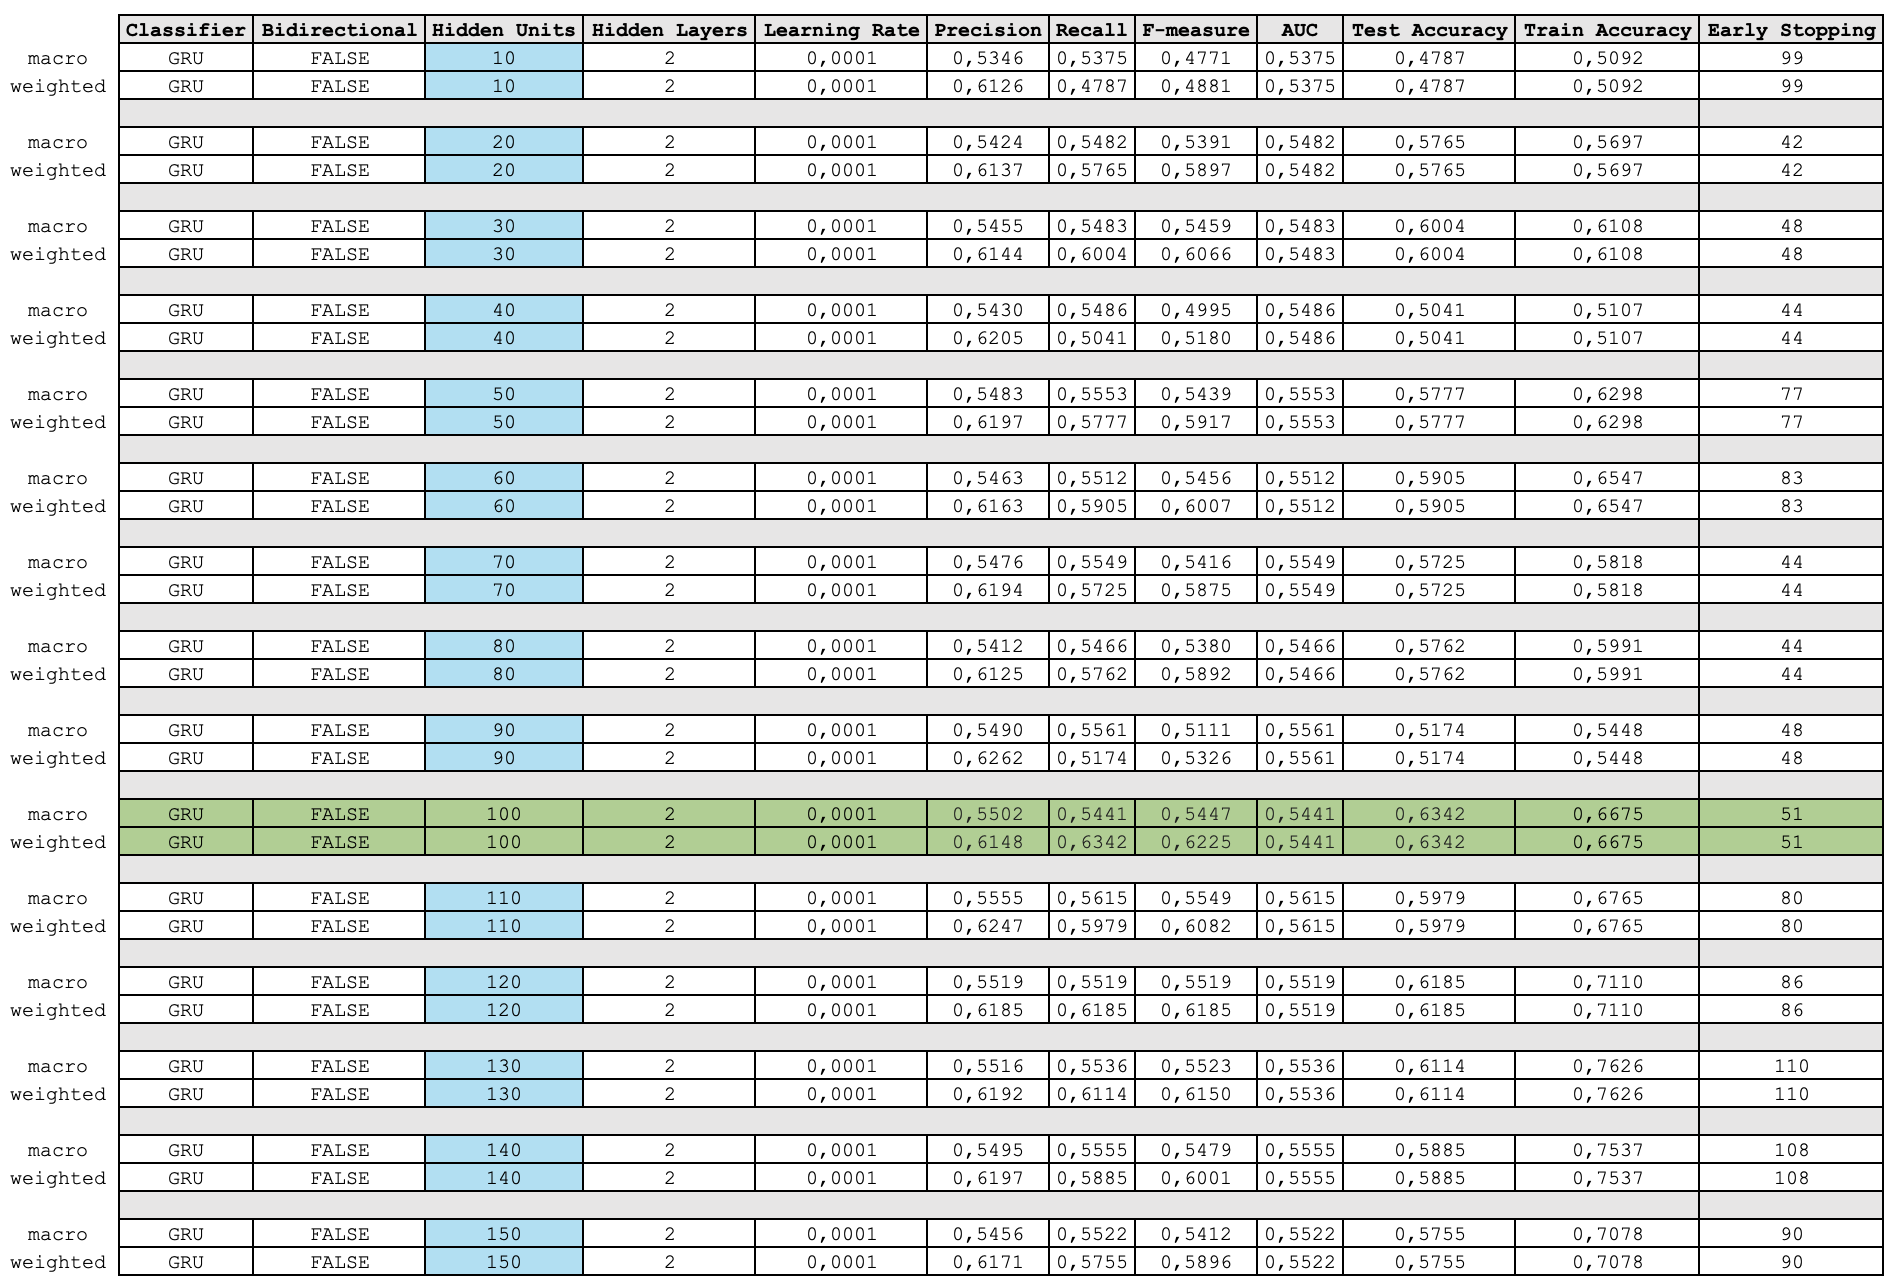
\includegraphics[width=1.2\linewidth]{appendix_tables/finger_units_table.png}}
\caption{Swipe Finger - Hidden Units Experiment Results}
\label{table:finger_units_table}
\end{table}

\begin{table}[!ht]
\centerline{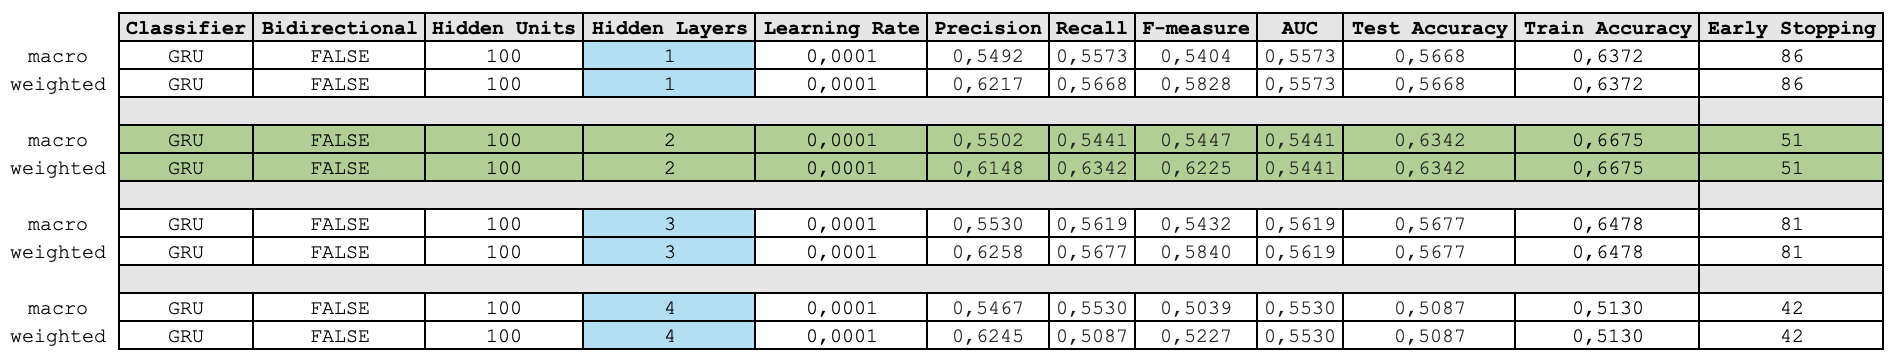
\includegraphics[width=1.2\linewidth]{appendix_tables/finger_layers_table.png}}
\caption{Swipe Finger - Hidden Layers Experiment Results}
\label{table:finger_layers_table}
\end{table}

\begin{table}[!ht]
\centerline{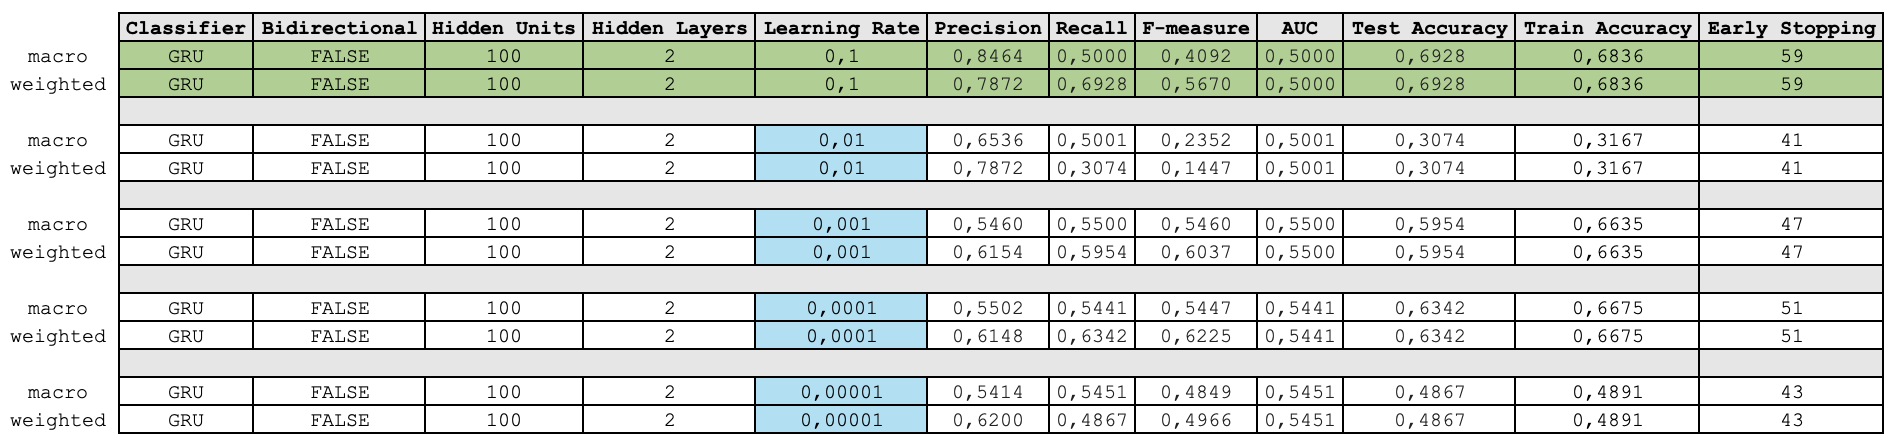
\includegraphics[width=1.2\linewidth]{appendix_tables/finger_lr_table.png}}
\caption{Swipe Finger - Learning Rate Experiment Results}
\label{table:finger_lr_table}
\end{table}

\end{document}
